\documentclass[11pt]{article}
	\usepackage{graphicx}
	\usepackage{hyperref}
	\usepackage{indentfirst}
	\usepackage[a4paper, tmargin=15mm, lmargin=20mm, rmargin=15mm, bmargin=15mm]{geometry}
	
	\hypersetup{
		colorlinks=true,
		urlcolor=cyan
	}
	
  \title{\textbf{An Exhaustive and Exhausting Guide to the Autochrome Lumière Process}}
  \author{John Hilty (\url{https://www.jonhilty.com})}
  \date{}
  
%  \addtolength{\topmargin}{-3cm}
%  \addtolength{\textheight}{3cm}
\begin{document}

\maketitle

\section{Introduction}

I started experimenting with making autochromes as far back as 2013, and they became my full time hobby in 2017. After three years and thousands of hours of experimentation, I think I'm finally at a point that I can publish the findings I've made thus far into a comprehensive guide. I believe in complete and total transparency, and it's my sincerest hopes that others can learn from what I've done and make their own autochromes too. The Lumiere Autochrome is a beautiful process, and deserves better than to be left behind merely as a distant colorful memory.\newline

\begin{center}
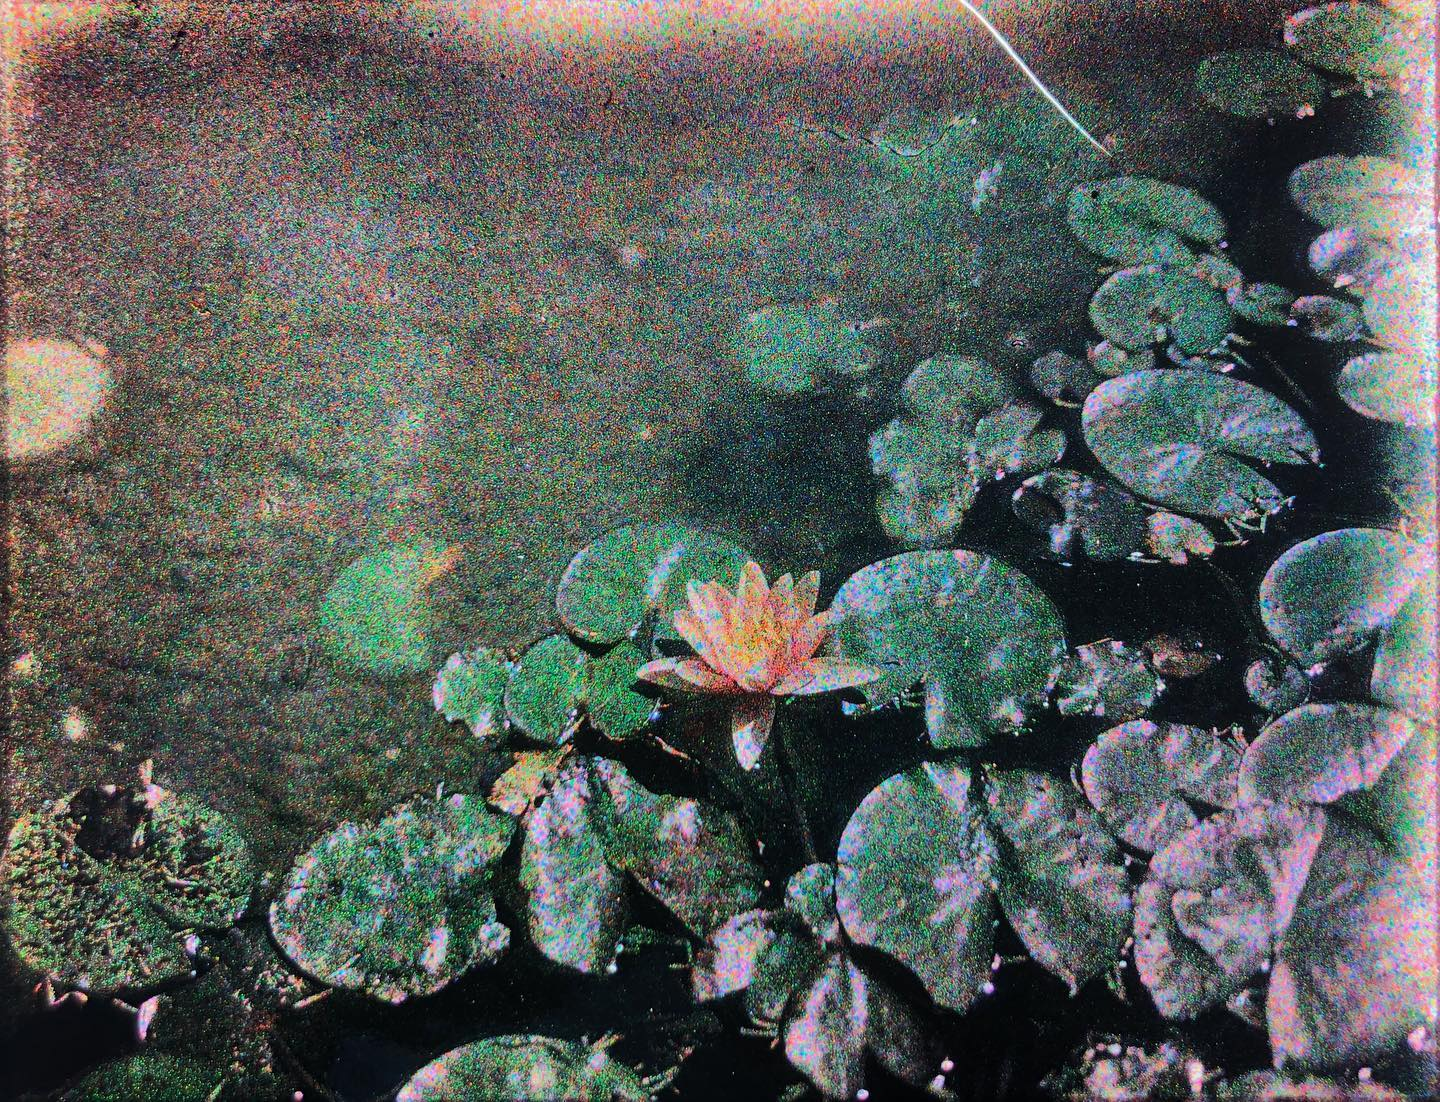
\includegraphics[width=4cm, height=4cm]{img/intro_1.jpg}
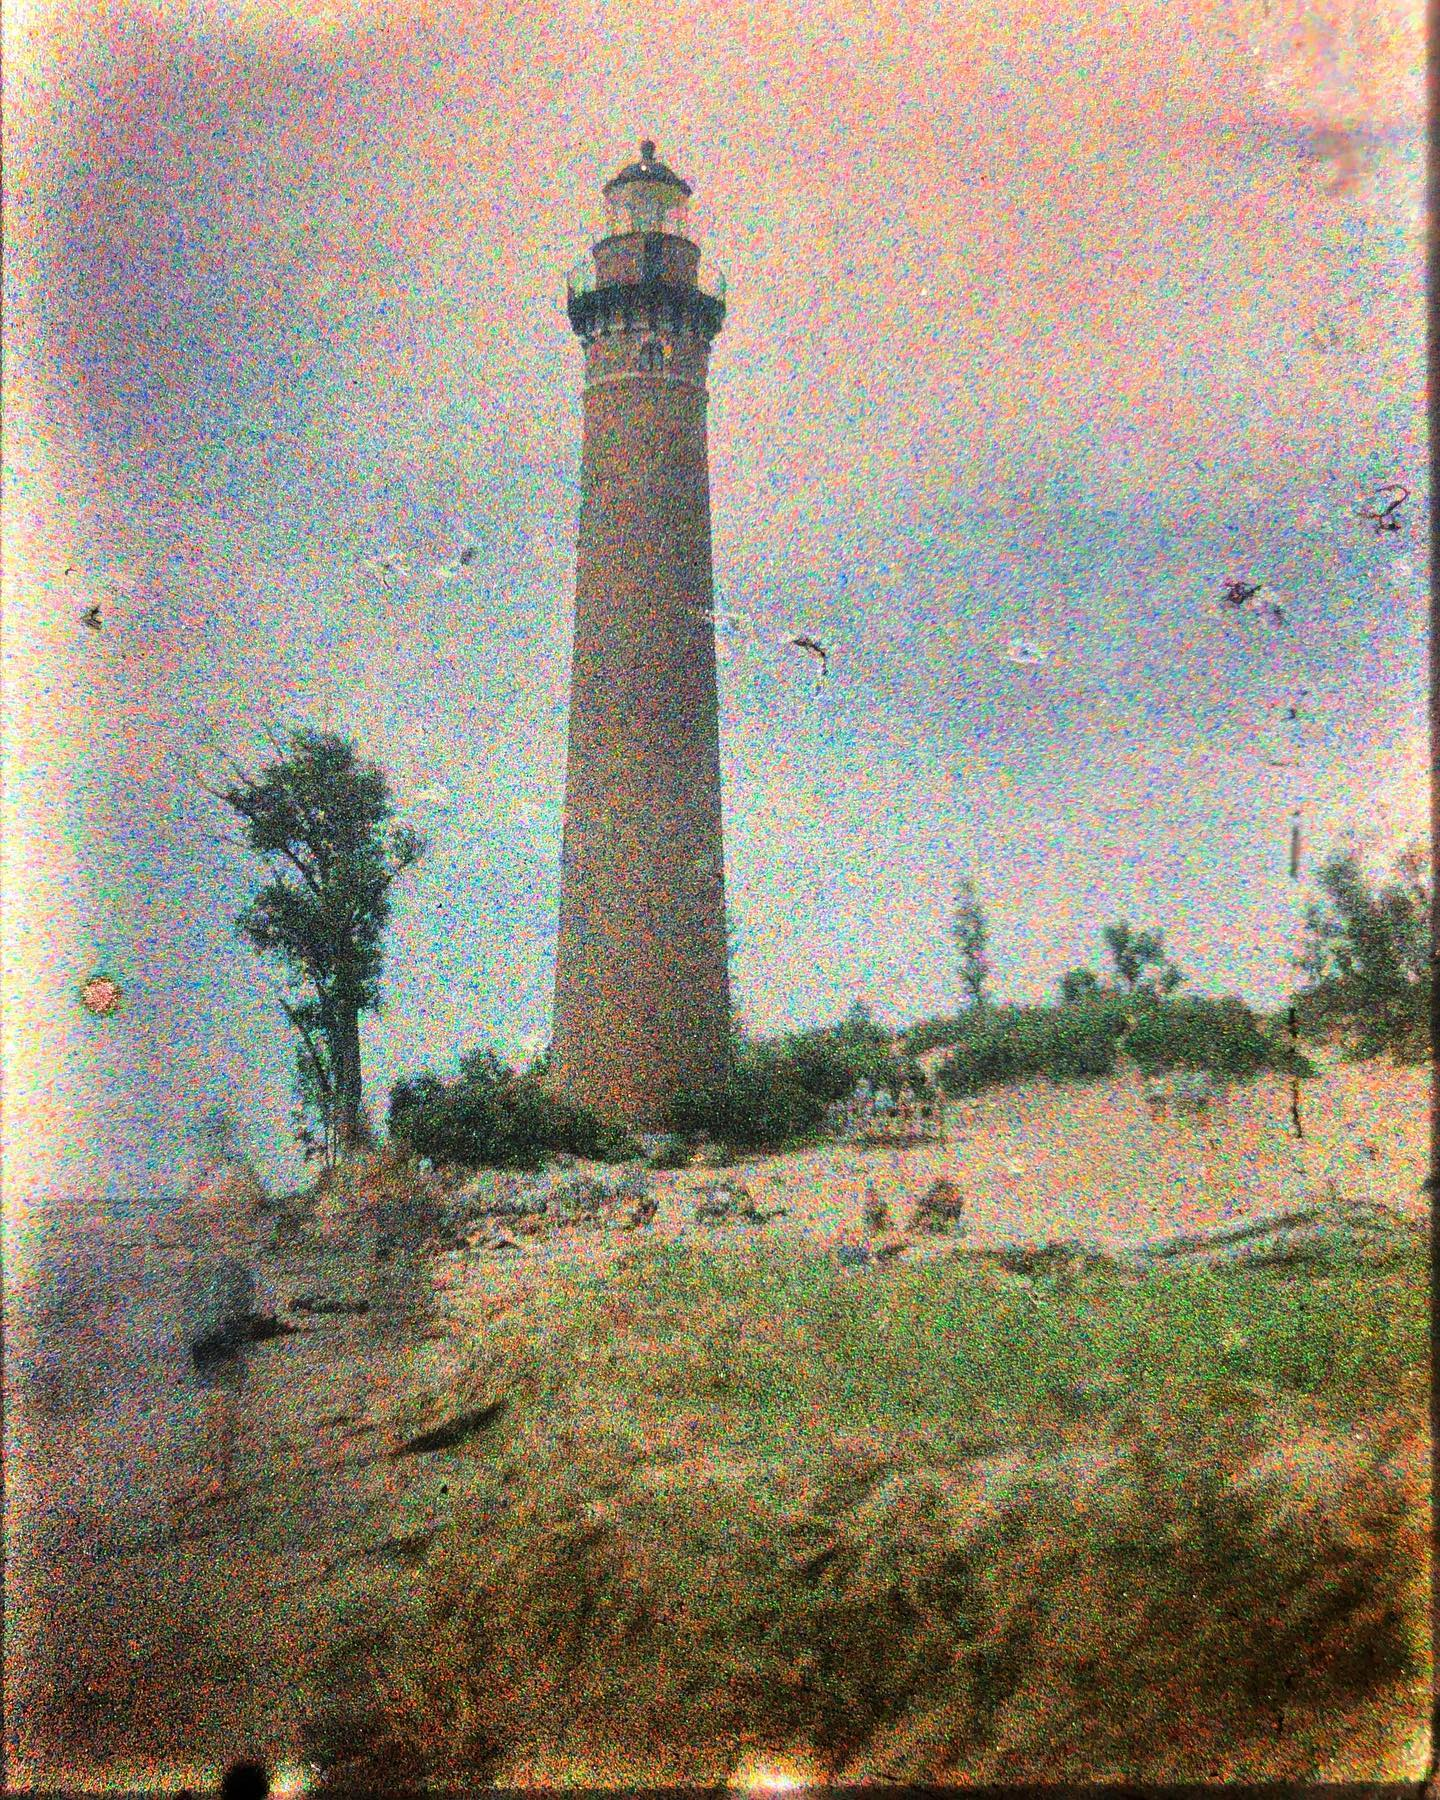
\includegraphics[width=4cm, height=4cm]{img/intro_2.jpg}
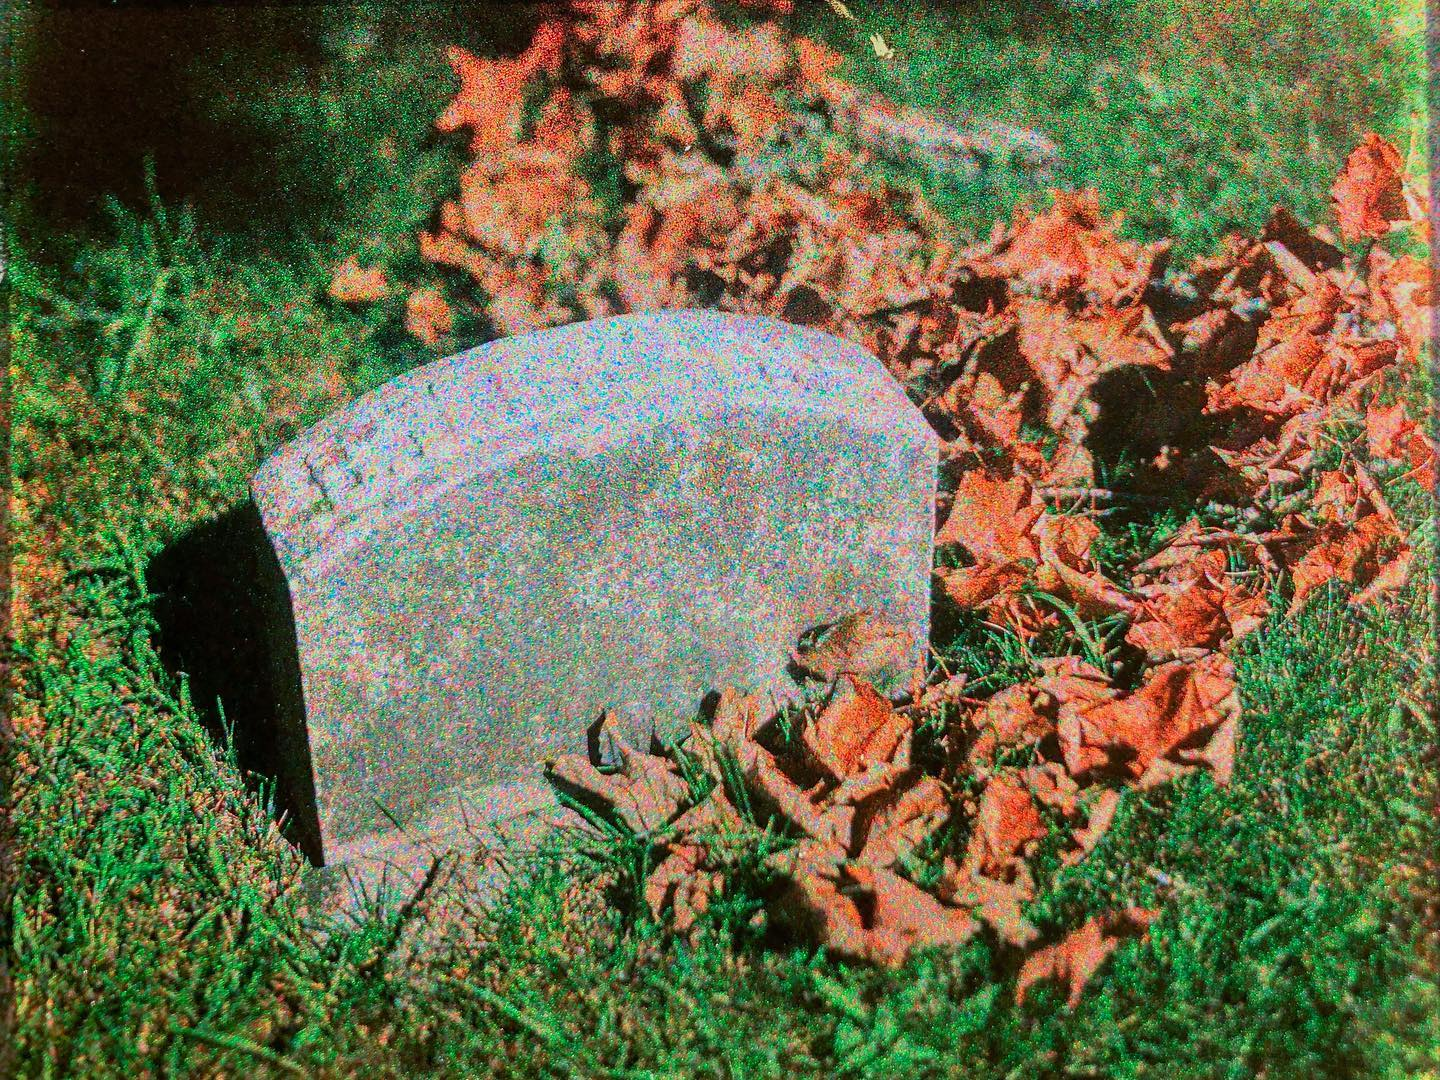
\includegraphics[width=4cm, height=4cm]{img/intro_3.jpg}
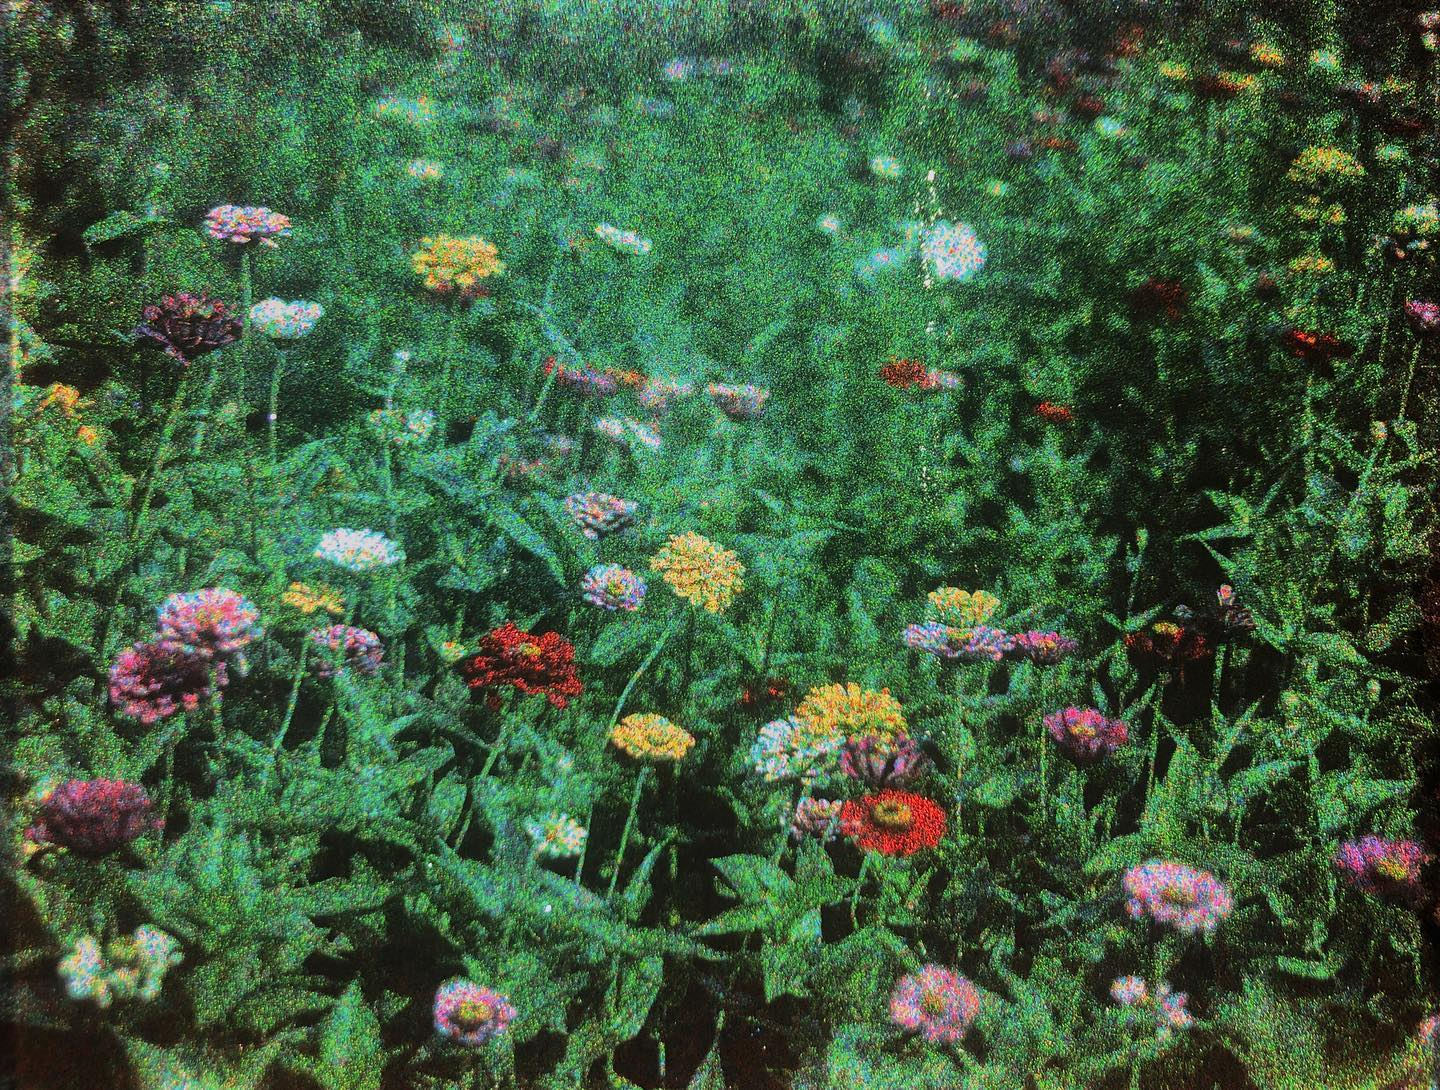
\includegraphics[width=4cm, height=4cm]{img/intro_4.jpg}
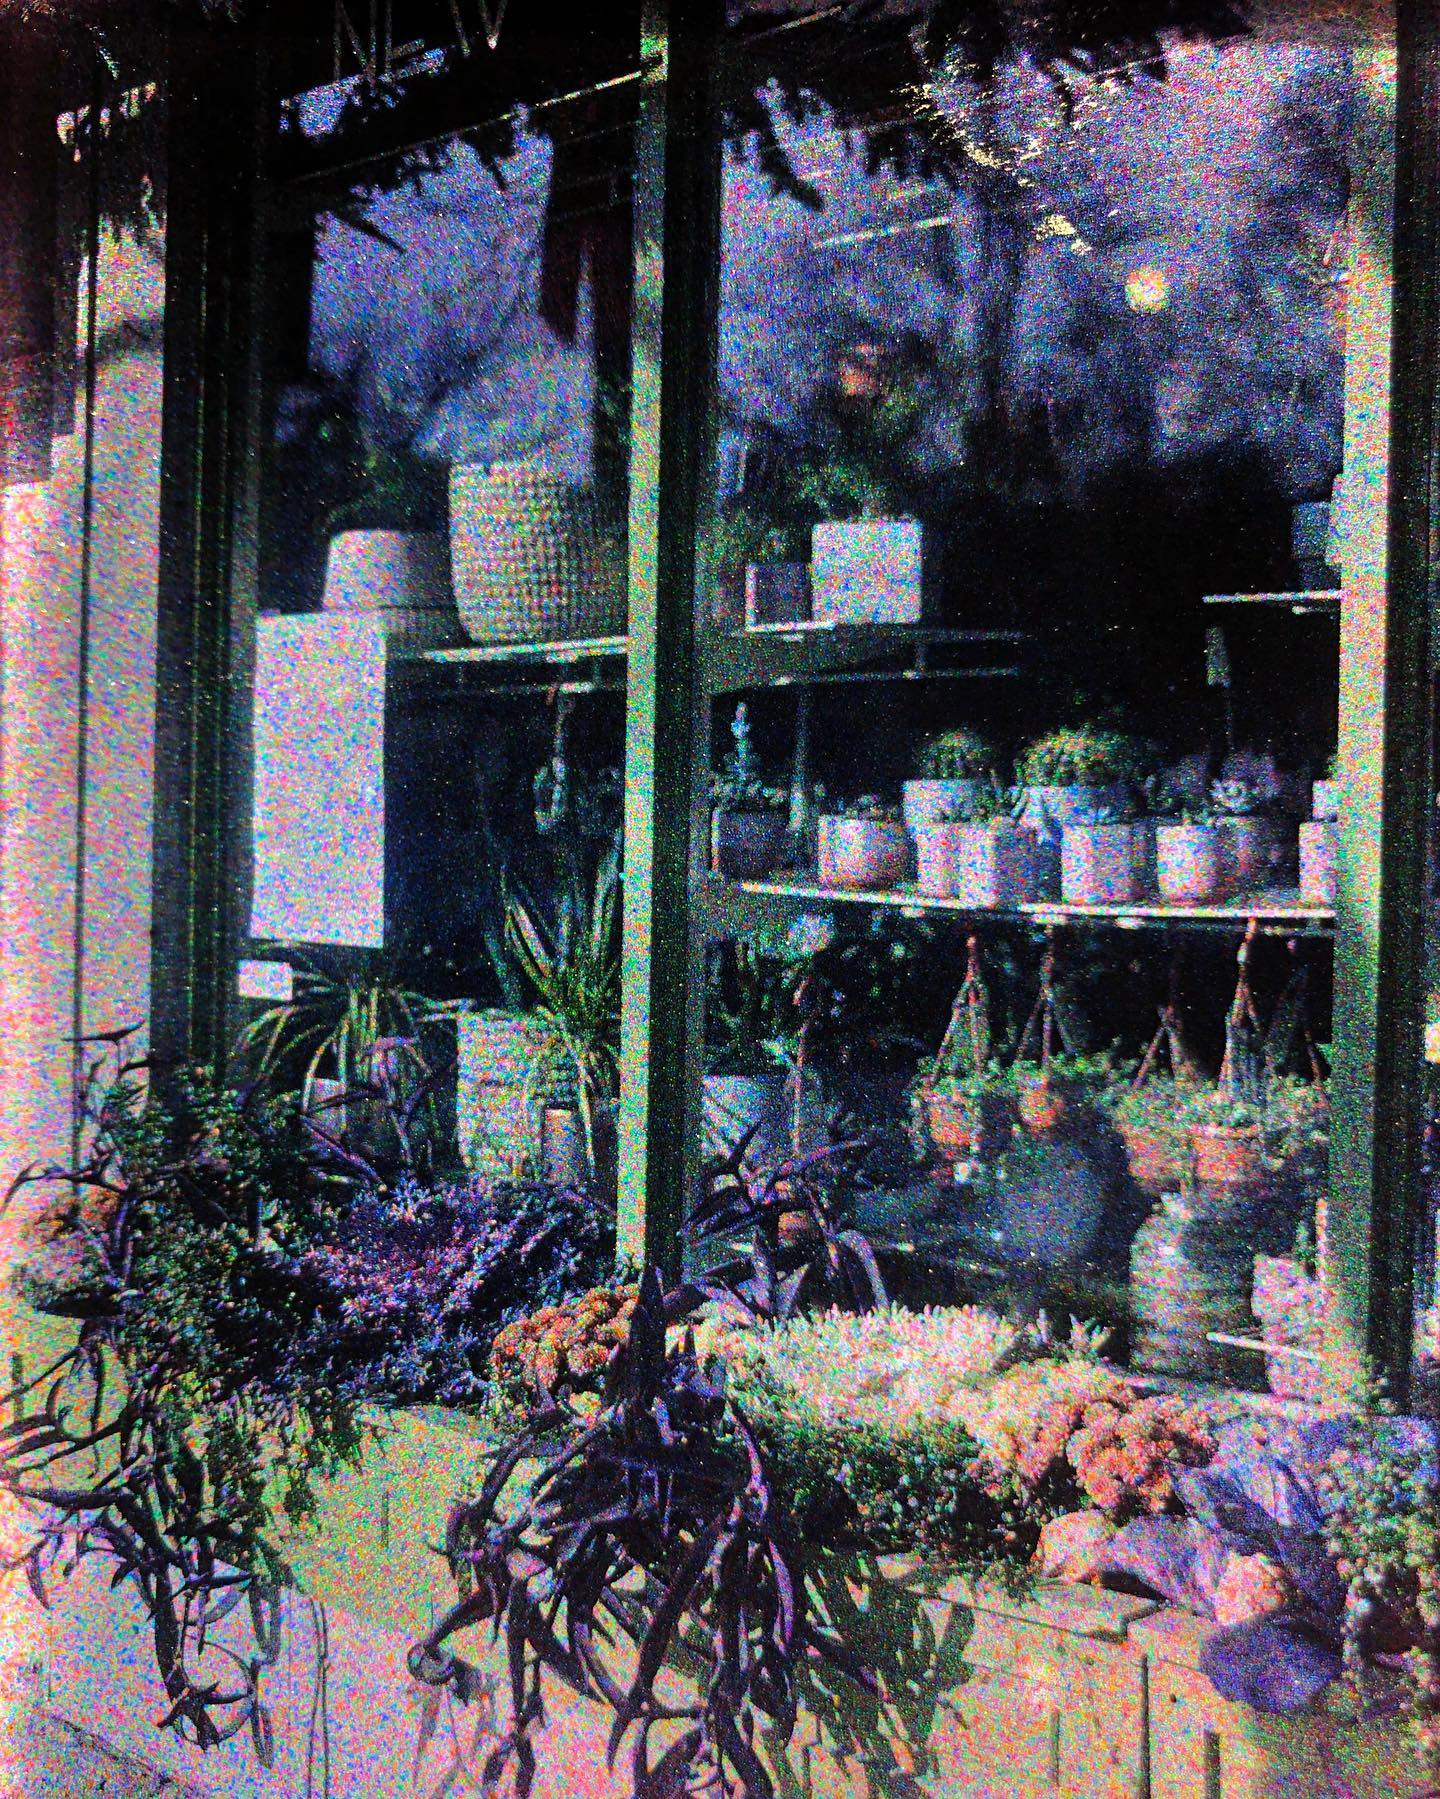
\includegraphics[width=4cm, height=4cm]{img/intro_5.jpg}
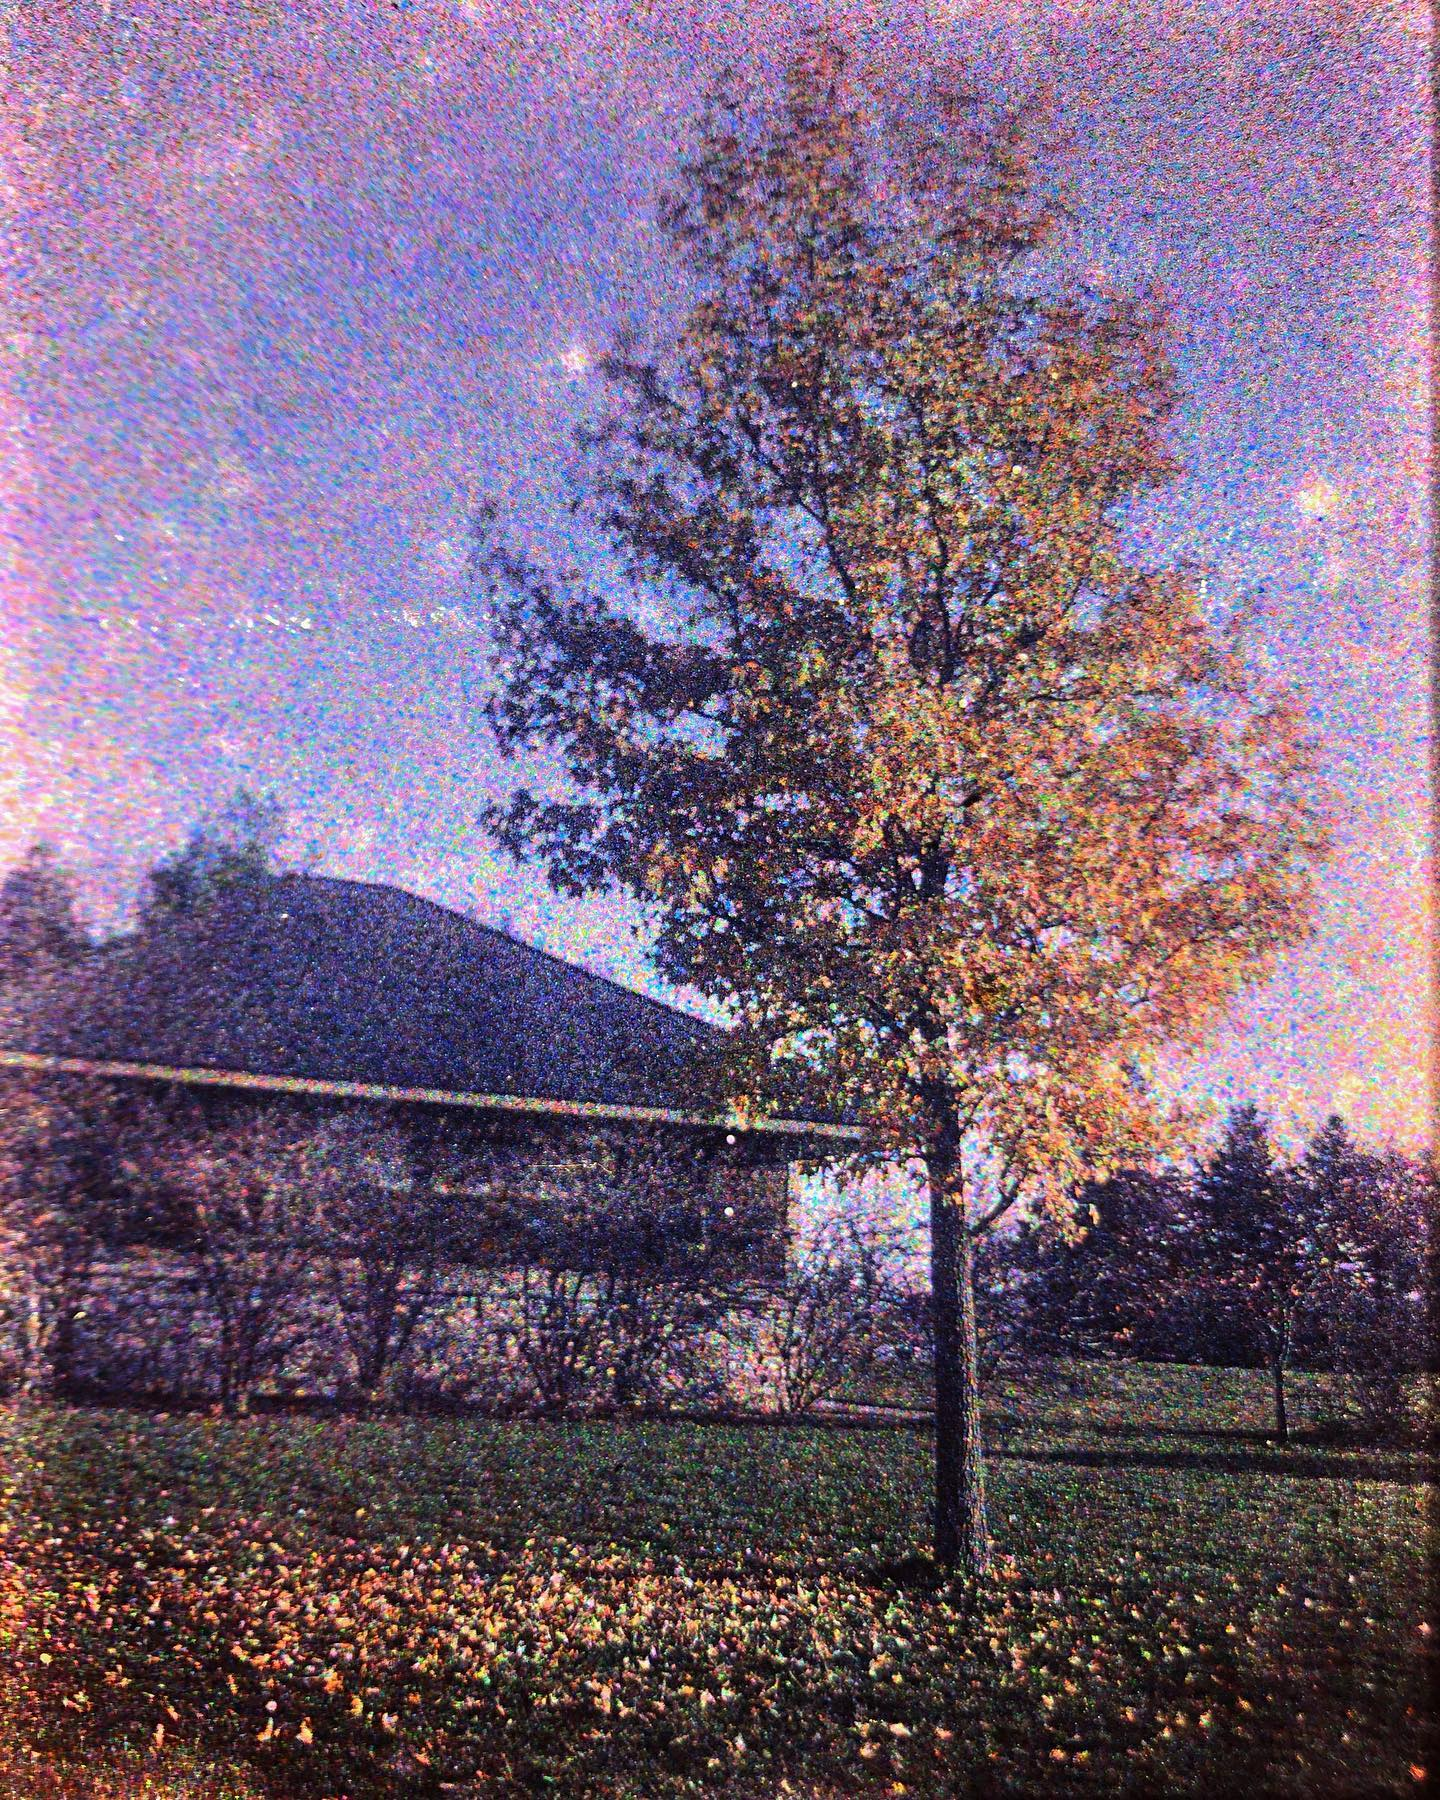
\includegraphics[width=4cm, height=4cm]{img/intro_6.jpg}
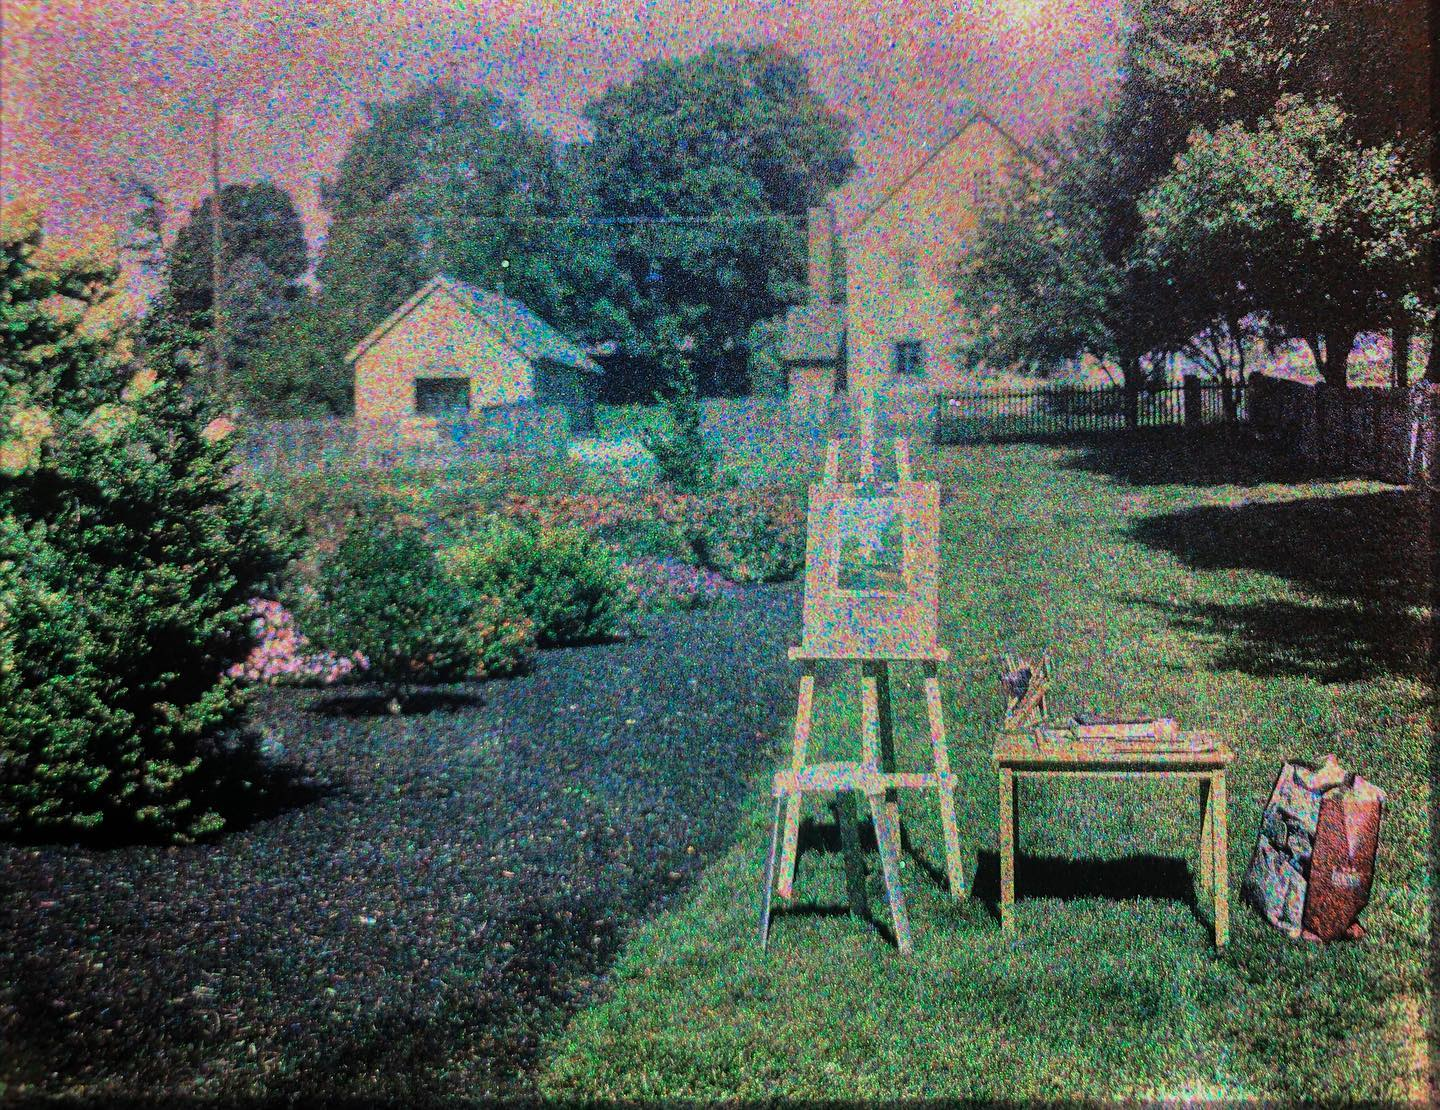
\includegraphics[width=4cm, height=4cm]{img/intro_7.jpg}
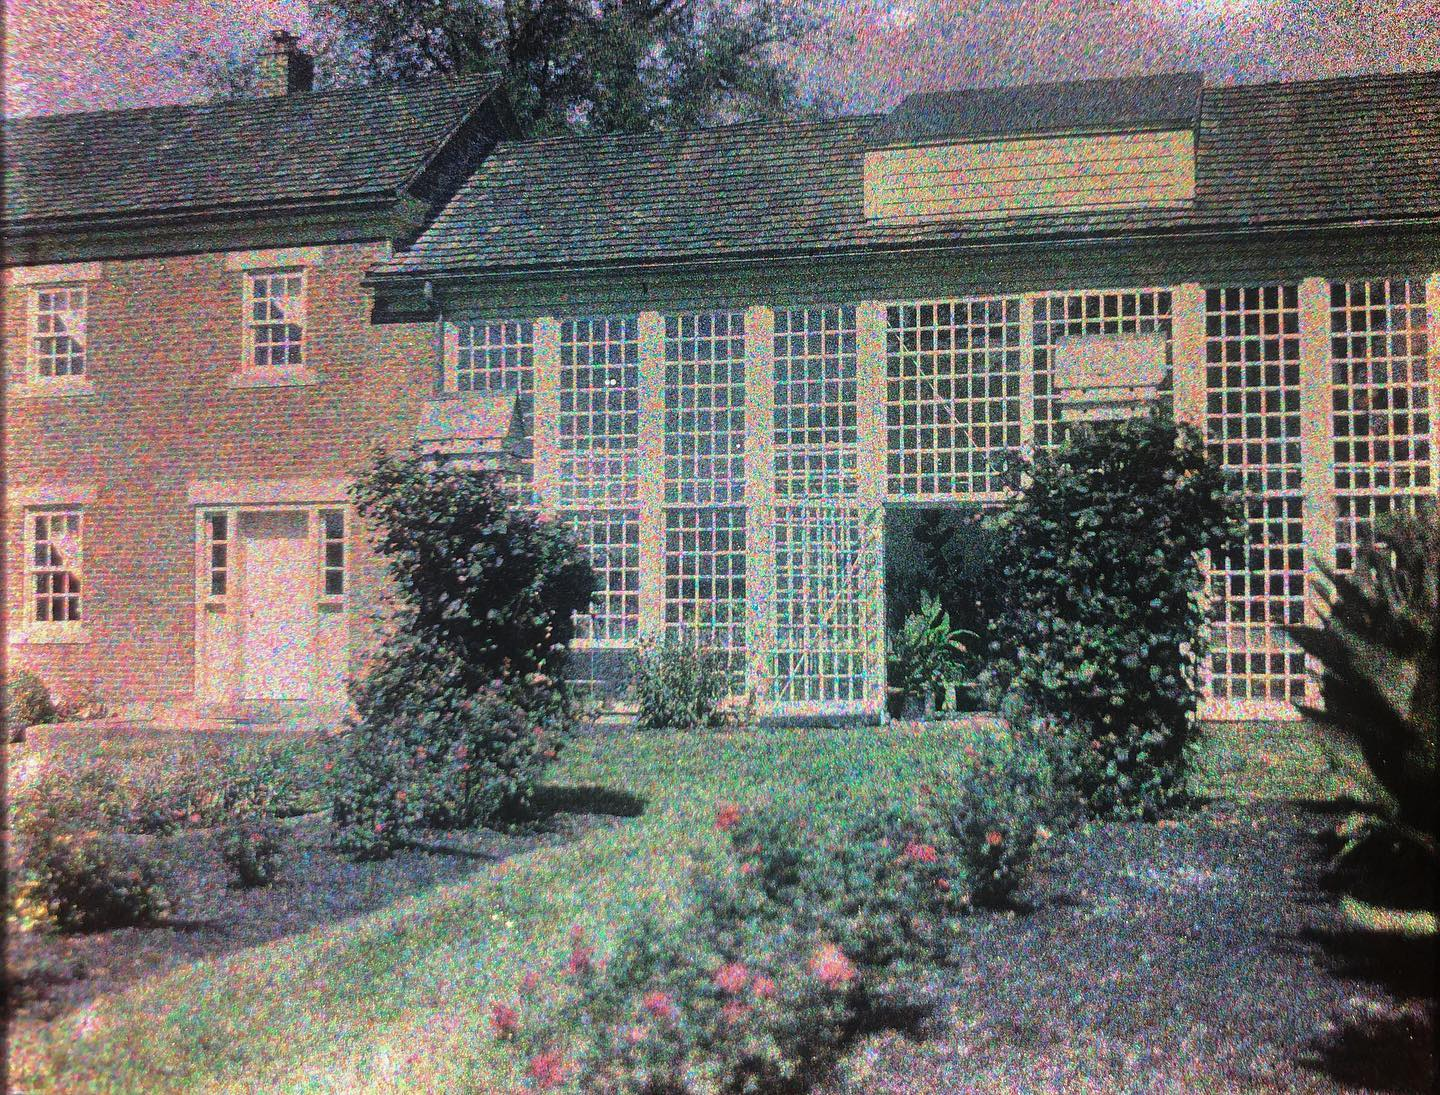
\includegraphics[width=4cm, height=4cm]{img/intro_8.jpg}
\end{center}

%\begin{description}
%\item[Part 1] - Manufacturing The Screen Plate
%\item[Part 2] - Making The Autochrome Emulsion
%\item[Part 3] - Exposure and Processing
%\end{description}

Many thanks to the authors of "The Lumière Autochrome: History, Technology, and Preservation", Jean-Paul Gandolfo and Bertrand Lavédrine. Their research was immeasurably valuable, and I owe much to them.\newline

Many additional thanks to Frédéric Mocellin, whose experimental work in autochromes heavily inspired my own. Thanks to Gavin McGuire, Nick Brandreth, Denise Ross, Jason Lane and Ron Mowrey. Their help over the years has been indispensable. Thanks to Katherine Greenleaf for coming up with a way more clever name for the guide.\newline

\pagebreak

\section{Manufacturing the Screen Plate}

The screen plate is the most unique and recognizable part of the autochrome process, but not necessarily the most difficult to make. Three portions of ordinary potato starch, dyed orange-red, green and violet, are mixed together to form a neutral reddish-grey, and then dusted onto a glass plate. The glass has been coated in a thin, optically clear latex-based varnish, and the potato starch sticks readily to it. The starch is compressed with a roller. This compression is necessary, as the amount of light that can pass through a flattened grain is vastly more than unattended, increasing the overall speed of the plate, as well as overall brightness and saturation. Charcoal is brushed on to fill in any open space in between the grains, and the whole thing is covered in a protective coating called the "second varnish".\newline

The final product is a very fine, random, color separation matrix, to which we would apply a panchromatic black and white emulsion. There is a ton of work that goes into each and every plate. Luckily, with a correct choice of second varnish, the screen can be reused indefinitely if an exposure doesn't work out.\newline

\subsection{Preparing the Starch (Optional)}

Ordinary potato starch can be used here. For most of my work, I've always used "Bob's Red Mill" brand potato starch.\newline

Original autochromes separated the smallest starch grains from the larger ones via levigation -- they mixed it with water, where the largest particles would fall out of suspension first. After a period of time, the water containing the smaller particles would be transferred to another container where they could settle out.\newline 

This separation is not strictly necessary, but will make the final resulting screen less grainy. All the plates featured in this post all use unsorted starch -- I have not yet made a screen plate with the finer stuff. I have sorted and dyed some of it, so I figured I'd include some notes here.\newline

To the right is a picture of my simple levigation apparatus. It consists of two 5 gallon buckets. The upper bucket has a ball valve mounted a few inches up from the bottom. To begin, I add a full 1L measuring cup of potato starch to the bottom of the upper bucket, and fill the thing nearly to the top with water from a hose. I take a long spatula and thoroughly mix the starch into the water, making sure the thick deposit of starch at the bottom has all been suspended. The water is allowed to sit for 1 hour, and then the upper bucket's valve is opened, draining the contents into the lower bucket. The lower bucket is removed, and the starch allowed to settle overnight. After the starch has properly settled, the water can poured out without much loss of product, since most of it is now stuck in a thick layer on the bottom. The sorted starch can be collected and dried.\newline

\begin{center}
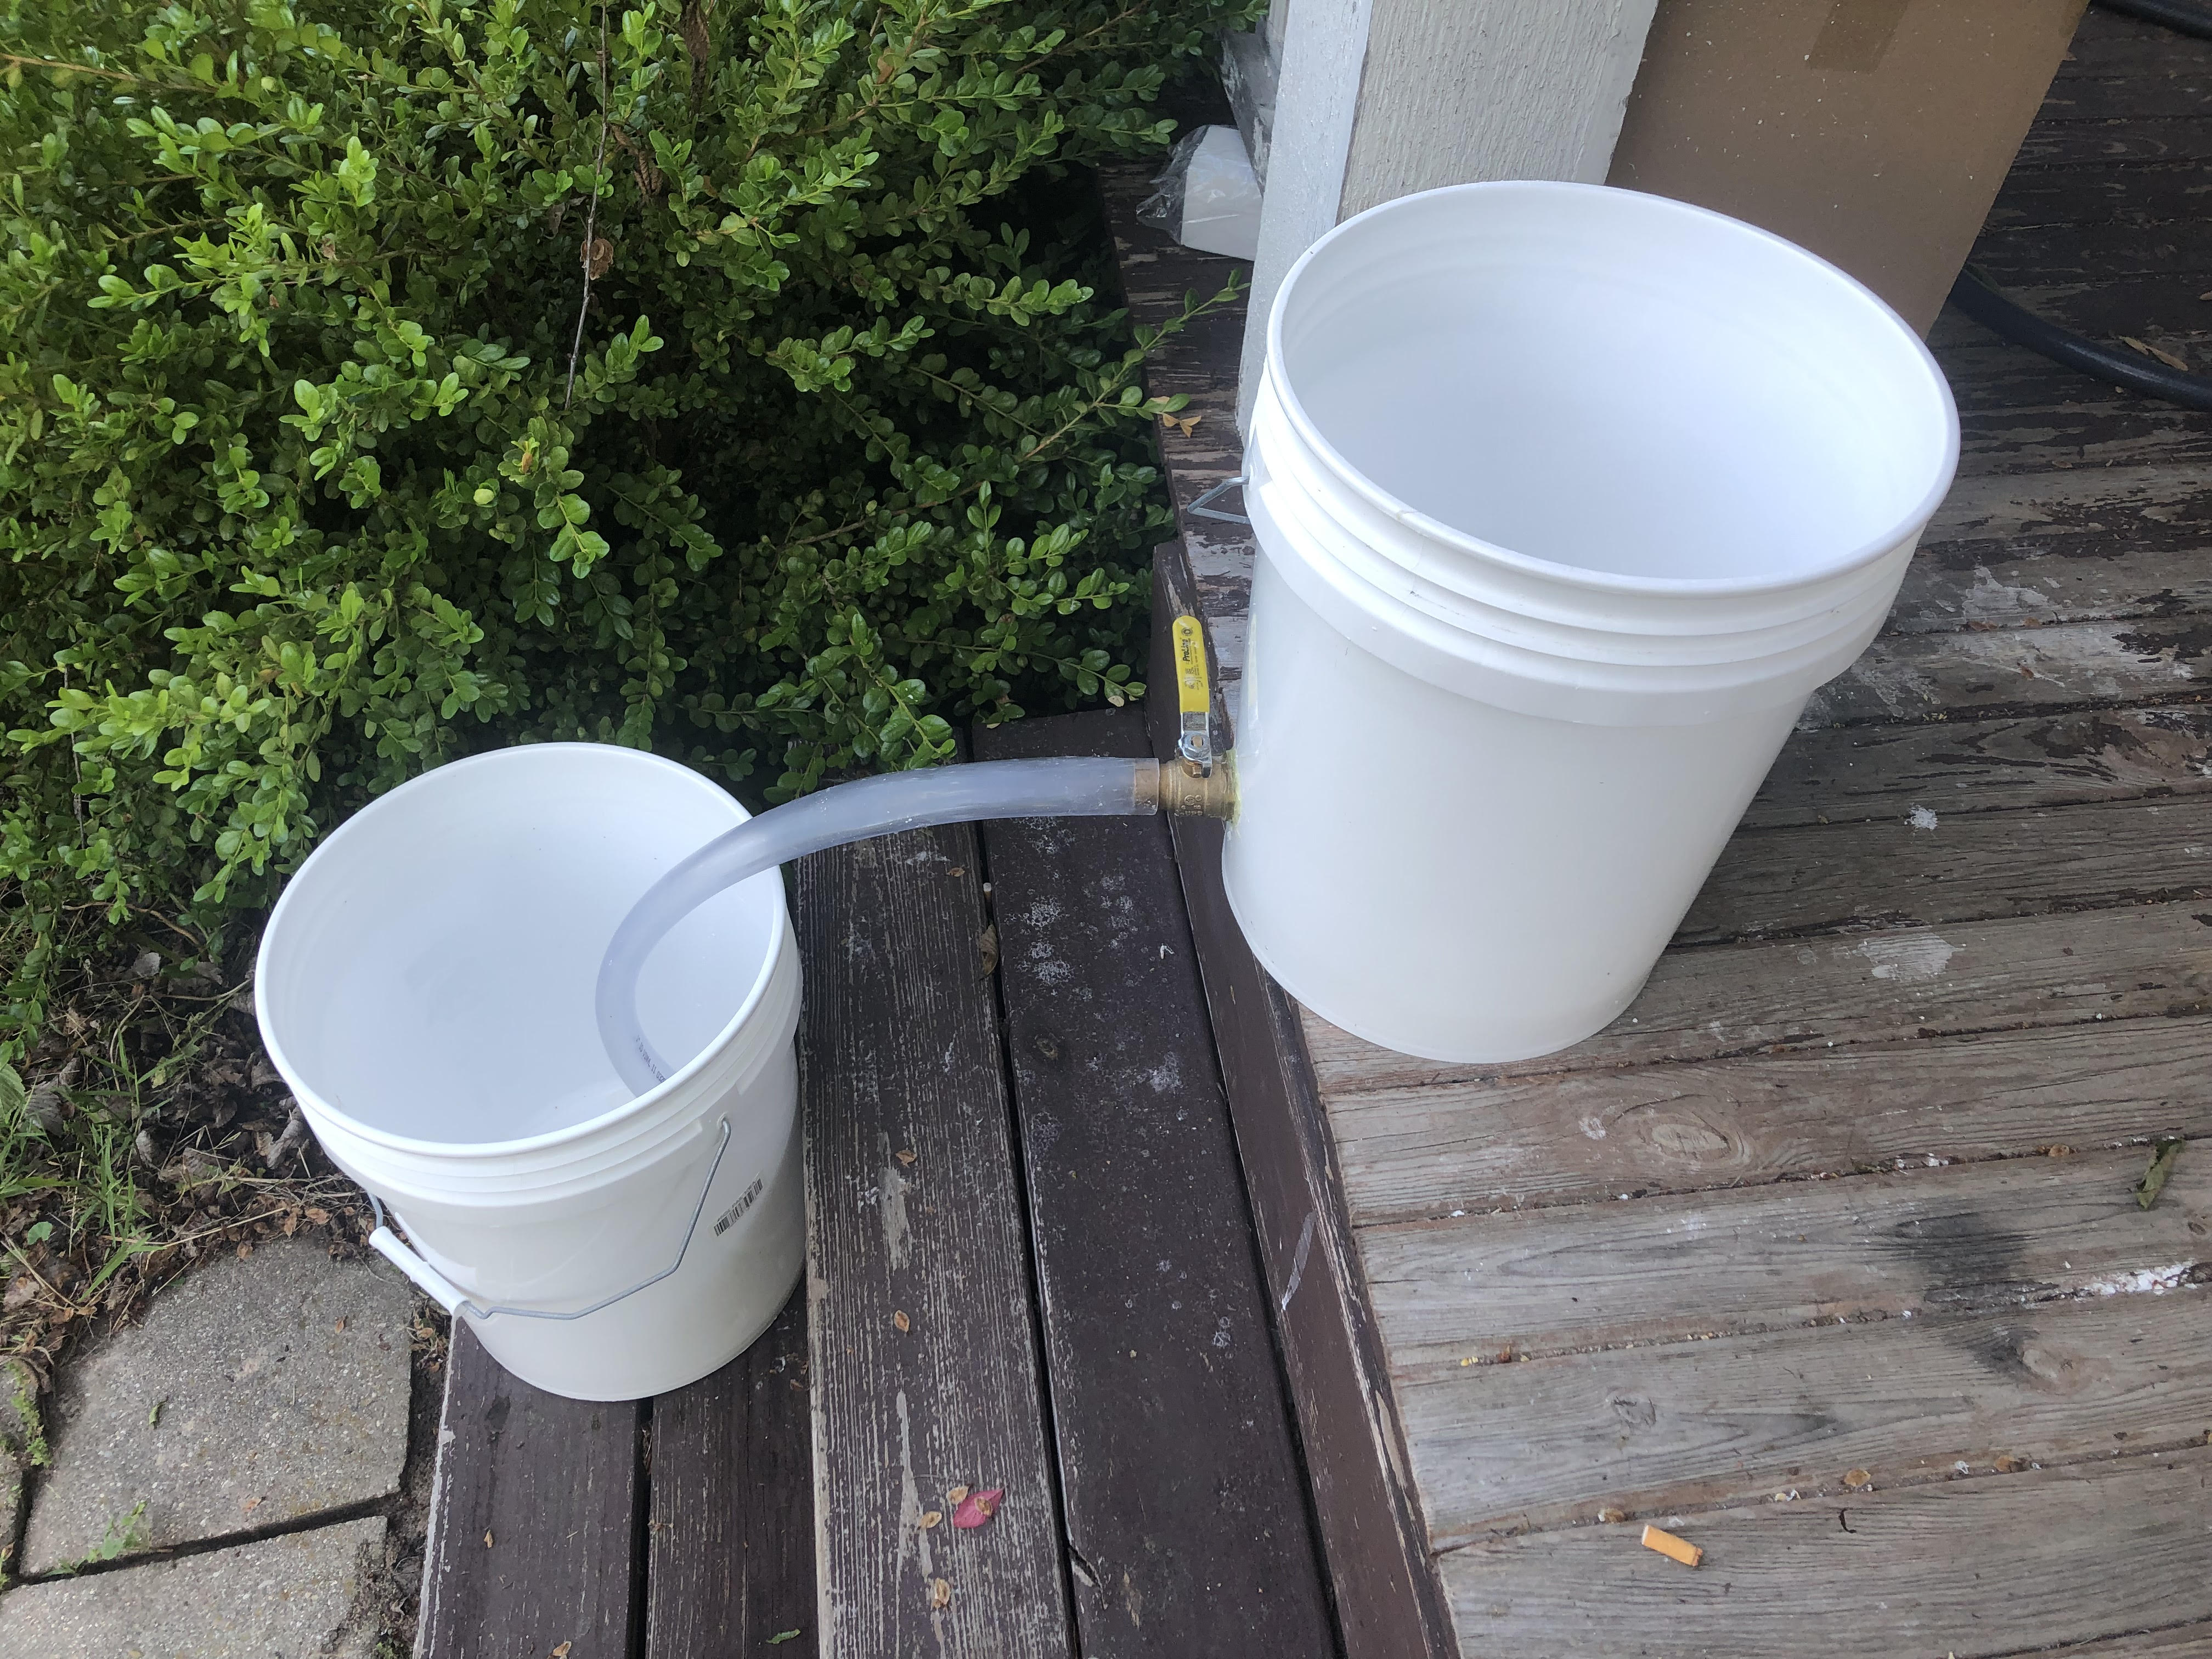
\includegraphics[height=7cm]{img/part1_1.jpg}
\end{center}

Recovery is quite low, so obtaining a reasonable amount of starch to dye will take several times. Usually I'll repeat the process with a second lower bucket using the same batch of starch in the upper bucket. Recover is even lower than the first time, and I figured additional runs will yield vastly diminished returns.\newline

\begin{center}
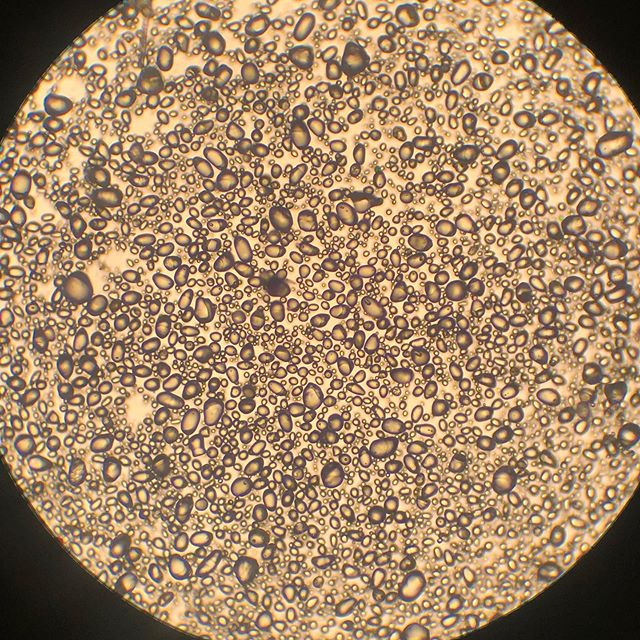
\includegraphics[width=5cm, height=5cm]{img/part1_2.jpg}
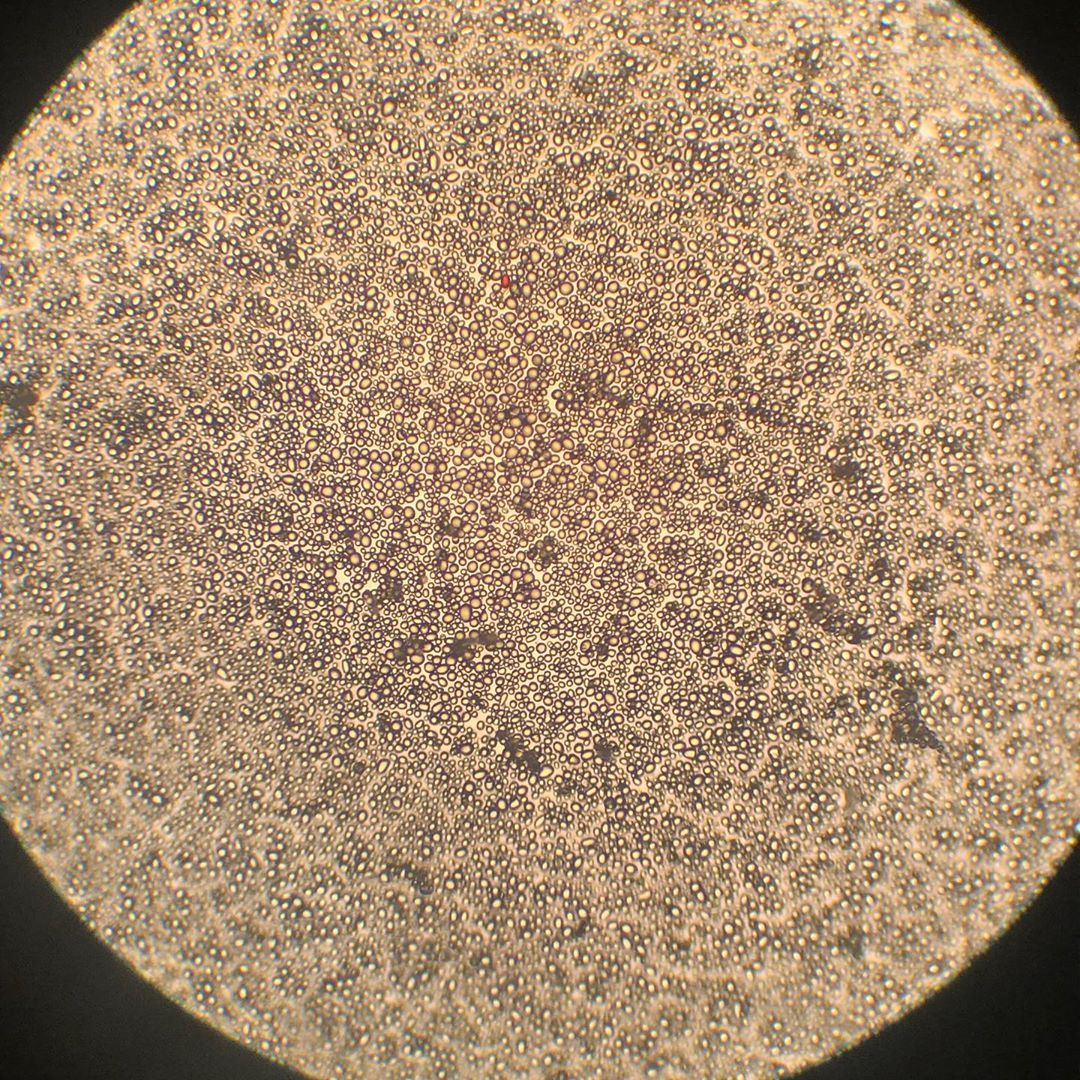
\includegraphics[width=5cm, height=5cm]{img/part1_3.jpg}
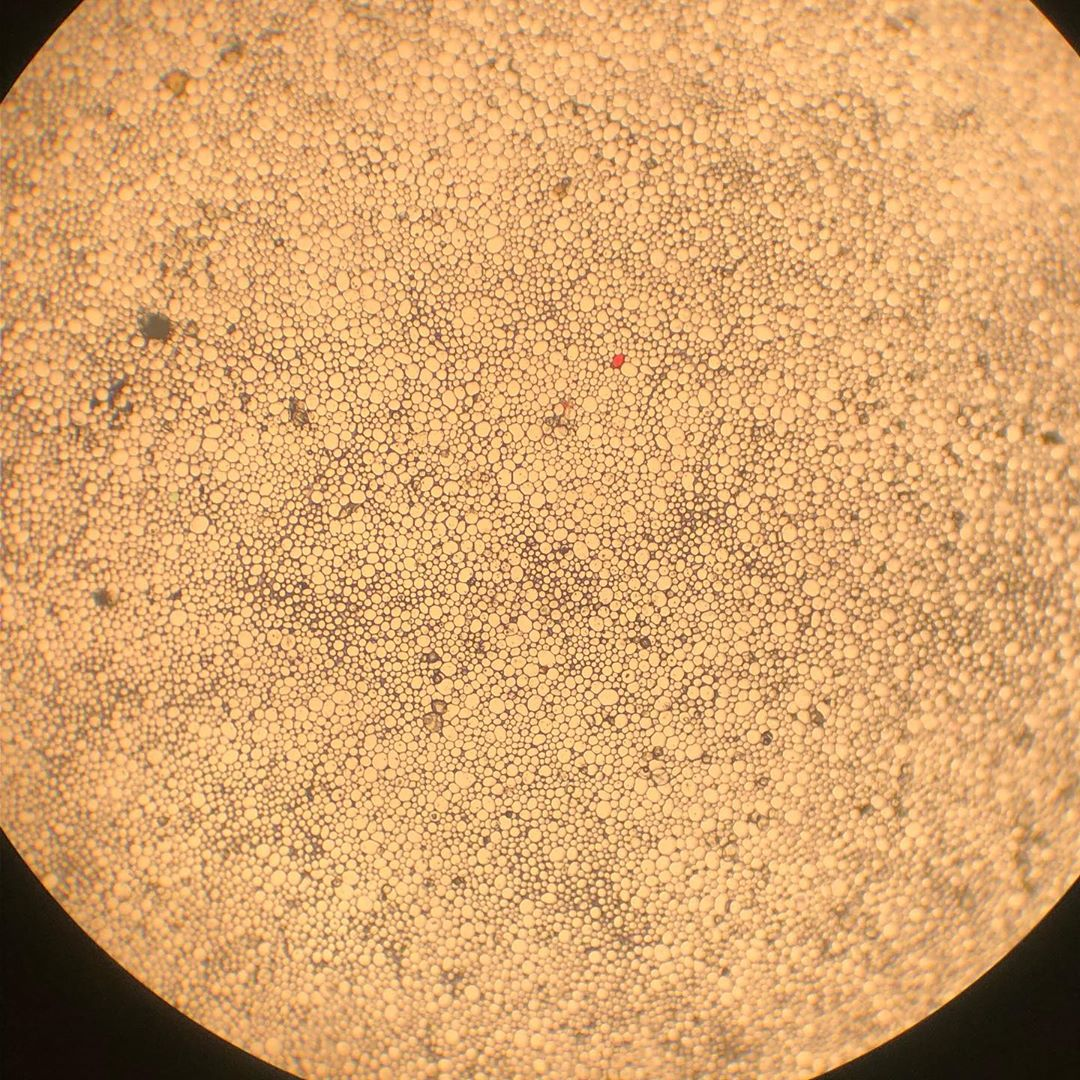
\includegraphics[width=5cm, height=5cm]{img/part1_4.jpg}
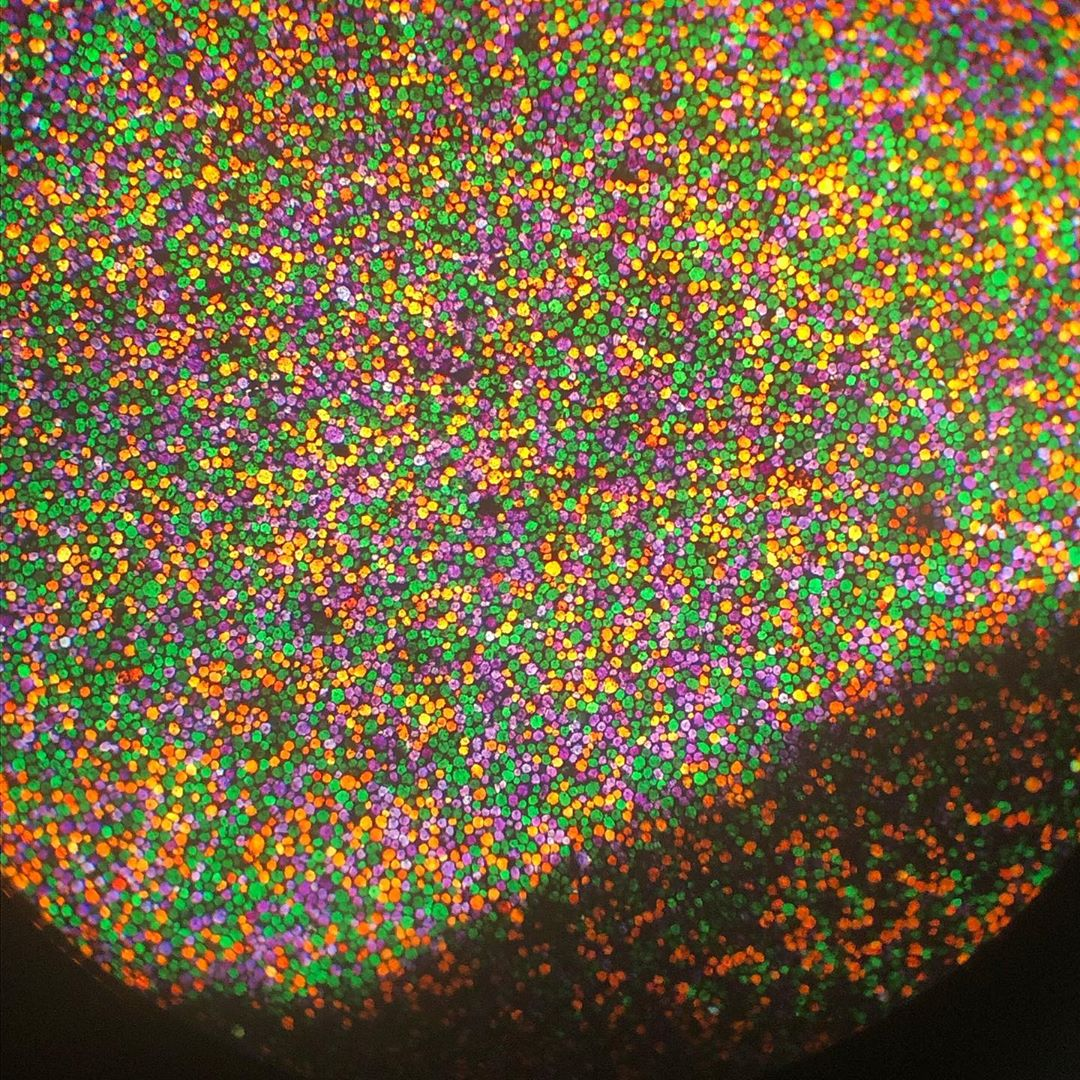
\includegraphics[width=5cm, height=5cm]{img/part1_5.jpg}
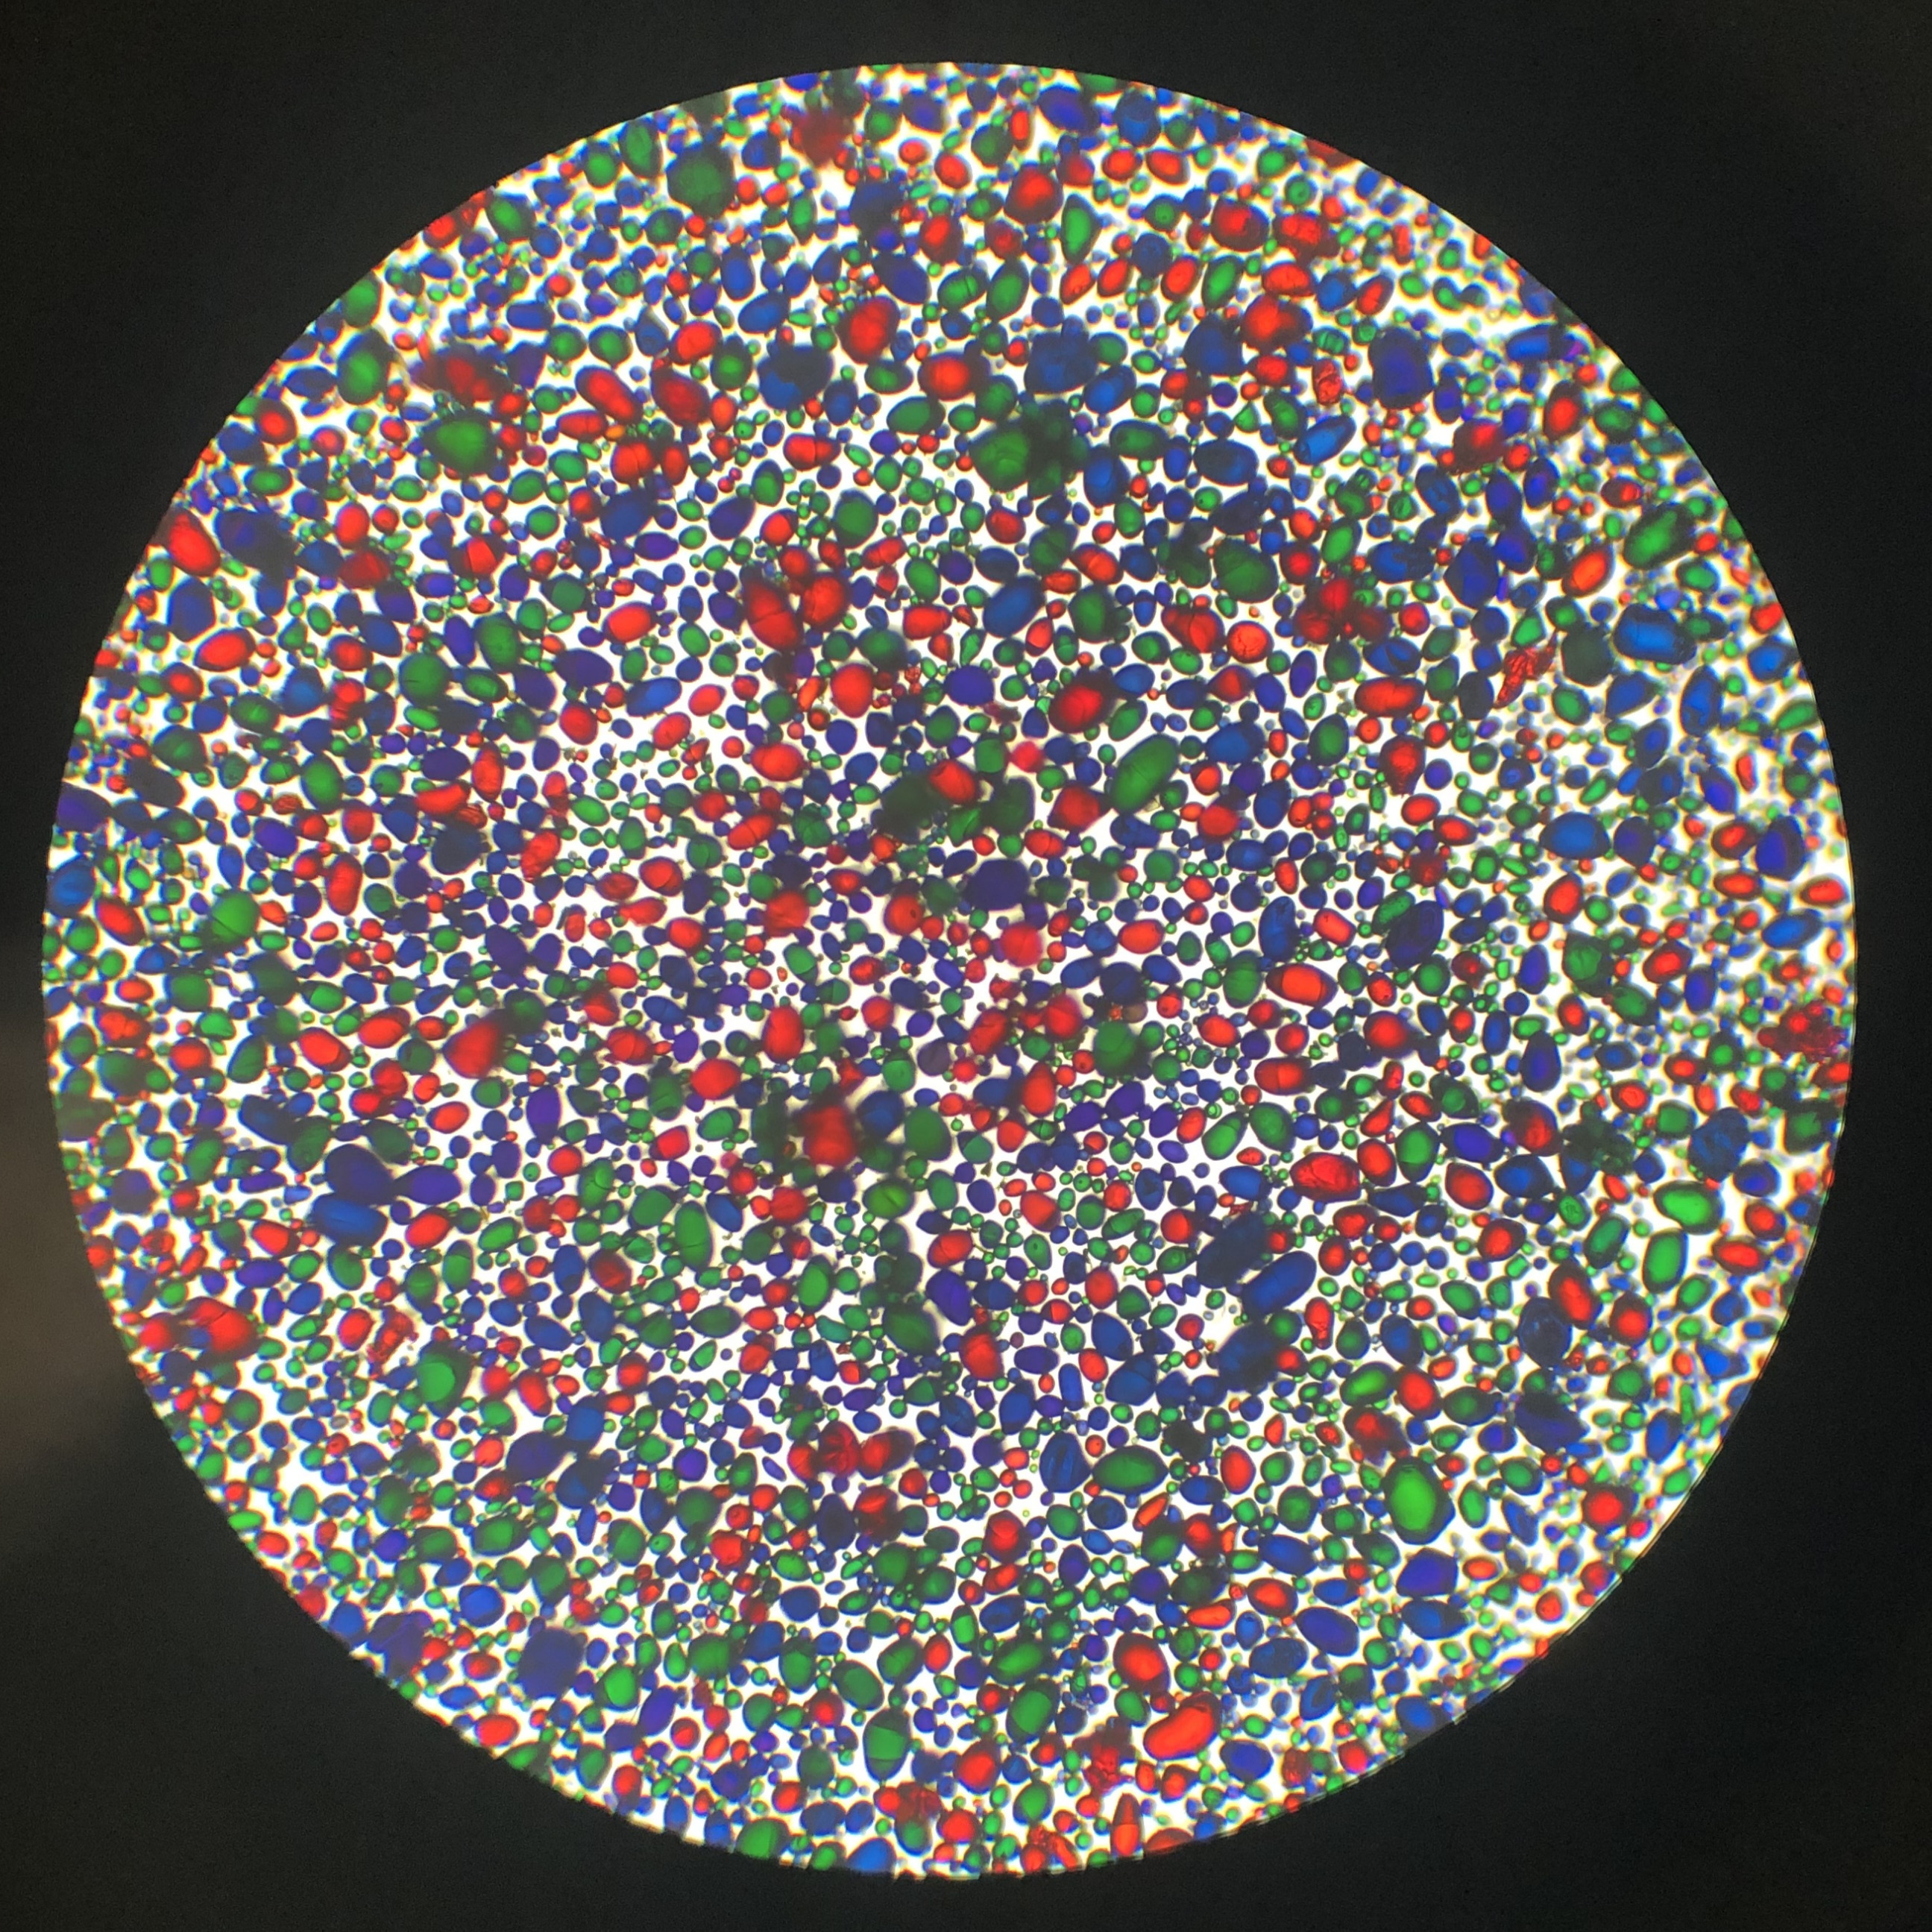
\includegraphics[width=5cm, height=5cm]{img/part1_6.jpg}
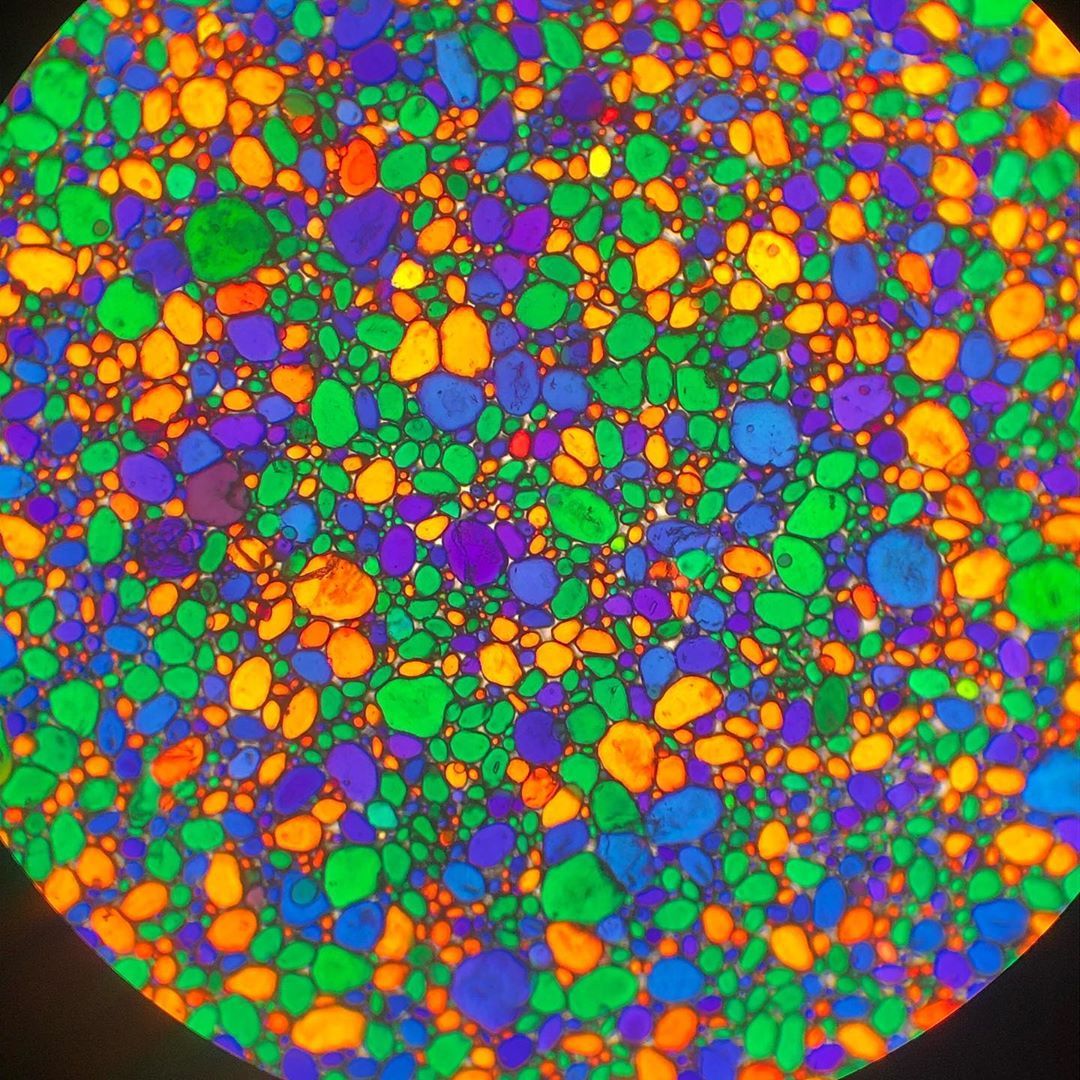
\includegraphics[width=5cm, height=5cm]{img/part1_7.jpg}
\end{center}

\subsection{Dyeing The Starch}

Whether you chose to sort or not, the next step here is to dye the starch a few different colors. The original dye formulas can be found in various places online, and I tried to stay as faithful as I could to them. The red and violet dyes are more or less the same, just scaled down quite a bit. I've found, at least with the dyes I sourced, that the green starch came out quite a bit more yellow than it should. I increased the amount of blue dye and decreased the amount of yellow to hopefully make it slightly more green.\newline

Over time, I also started omitting a few other extraneous steps that were in the original Lumière operating procedure -- I do not heat the violet dye solution (my now purple equipment is a testament to the fact that it stains quite well enough as it is), and I do not add ammonia or sodium sulfate to the green starch. The ammonia never seemed to alter the colors in any way, and the sodium sulfate tended to crystalize into large white chunks that contaminated the green starch.\newline

\noindent
\begin{tabular}{|l|c|l|c|l|c|}
	\hline
	\multicolumn{2}{|c|}{Orange Starch} &
	\multicolumn{2}{|c|}{Green Starch} &
	\multicolumn{2}{|c|}{Violet Starch} \\
	\hline
	Erythrosine & 11.2g & Tartrazine & 12g & Crystal Violet & 6.4g \\
	\hline
	Rose Bengal & 2g & Patent Blue V & 7.5g & Malachite Green & 0.9g \\
	\hline
	Tartrazine & 15.2g & - & & - & \\
	\hline
	Water & 150mL & Water & 150mL & Water & 150mL \\
	\hline
\end{tabular}\newline

I first dissolve the dyes into 150mL of water in a 250mL beaker with magnetic mixing, and allow the dye to dissolve completely over 10-15 minutes or so. The green and violet solutions will be so dark that they appear black, and all of them become a bit syrupy. After I'm certain they're all dissolved, I slowly add 50 - 150g of starch into the beaker, still under magnetic stirring. After the addition, I give it a good hour of stirring before transferring the slop to my vacuum filtration setup. Early on I would use simple gravity filtration with a coffee filter, but vacuum filtration has several advantages -- Firstly, it removes the bulk of the dye much more quickly than via gravity (or a hand powered pump). Second, the quick removal of the dye from the starch tends to allow for a more consistent coloring, whereas gravity filtration causes some grains to be dyed more heavily than others. Even under a vacuum, removal of the thick dye solution can take 10 or 20 minutes -- patience is key.\newline

I would recommend collecting and saving the dye solution after filtration, as it can be reused at least once, and most likely a few times before you need to mix up a new one.\newline

After the starch has been collected and dried, you may find that it tends to clump up a bit. In particular, I tend to have the most trouble with the orange starch, as it forms tiny granules that stubbornly stuck together.\newline

\begin{center}
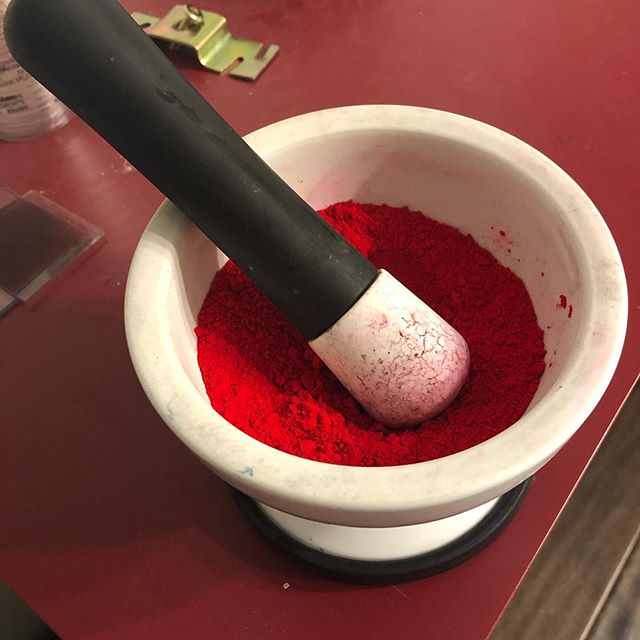
\includegraphics[width=3cm, height=3cm]{img/part1_8.jpg}
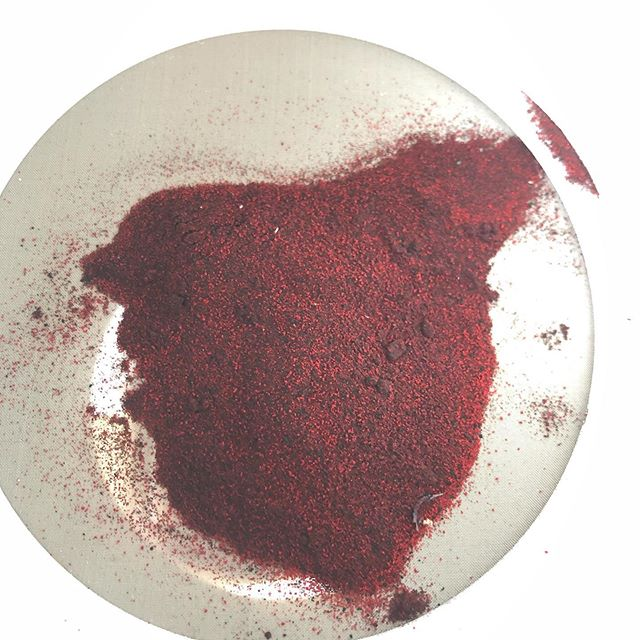
\includegraphics[width=3cm, height=3cm]{img/part1_9.jpg}
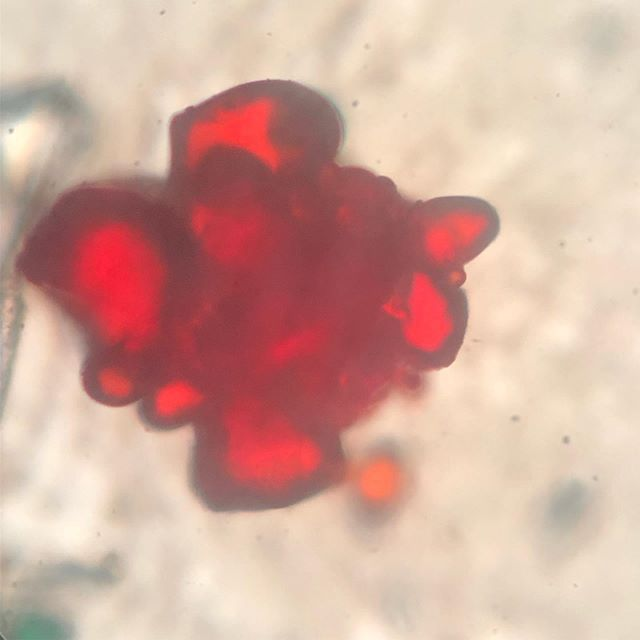
\includegraphics[width=3cm, height=3cm]{img/part1_10.jpg}
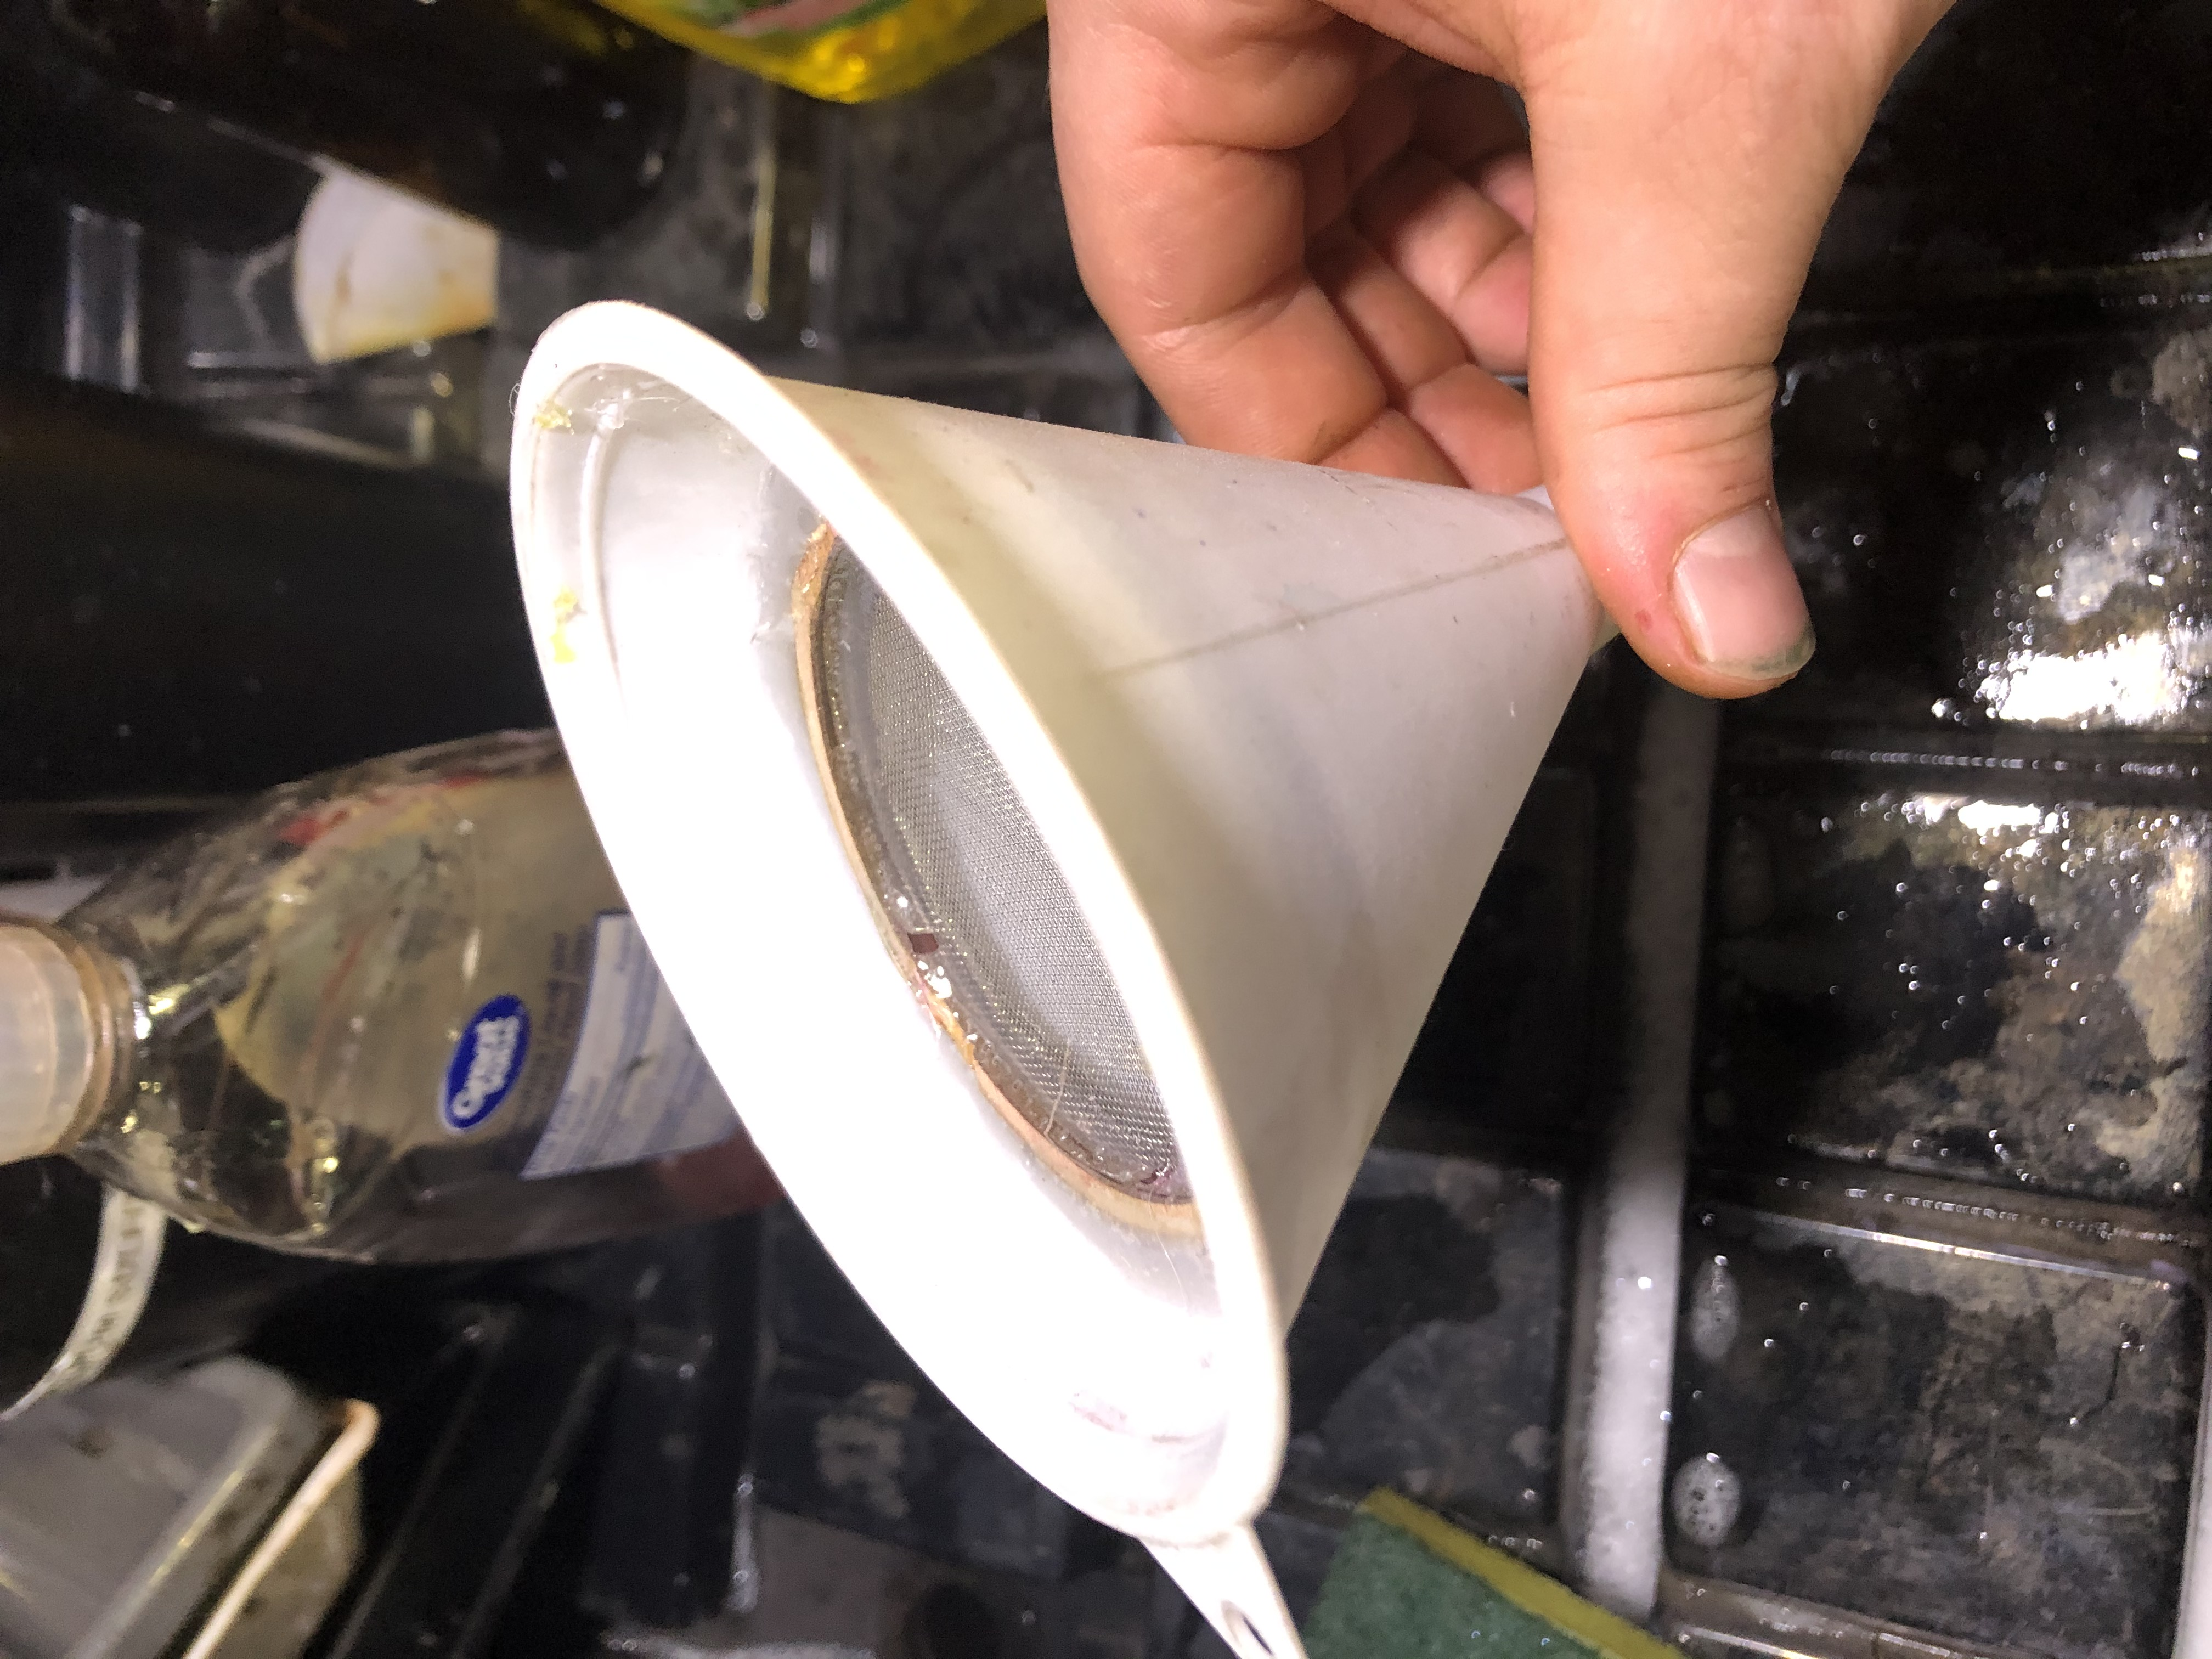
\includegraphics[width=3cm, height=3cm]{img/part1_11.jpg}
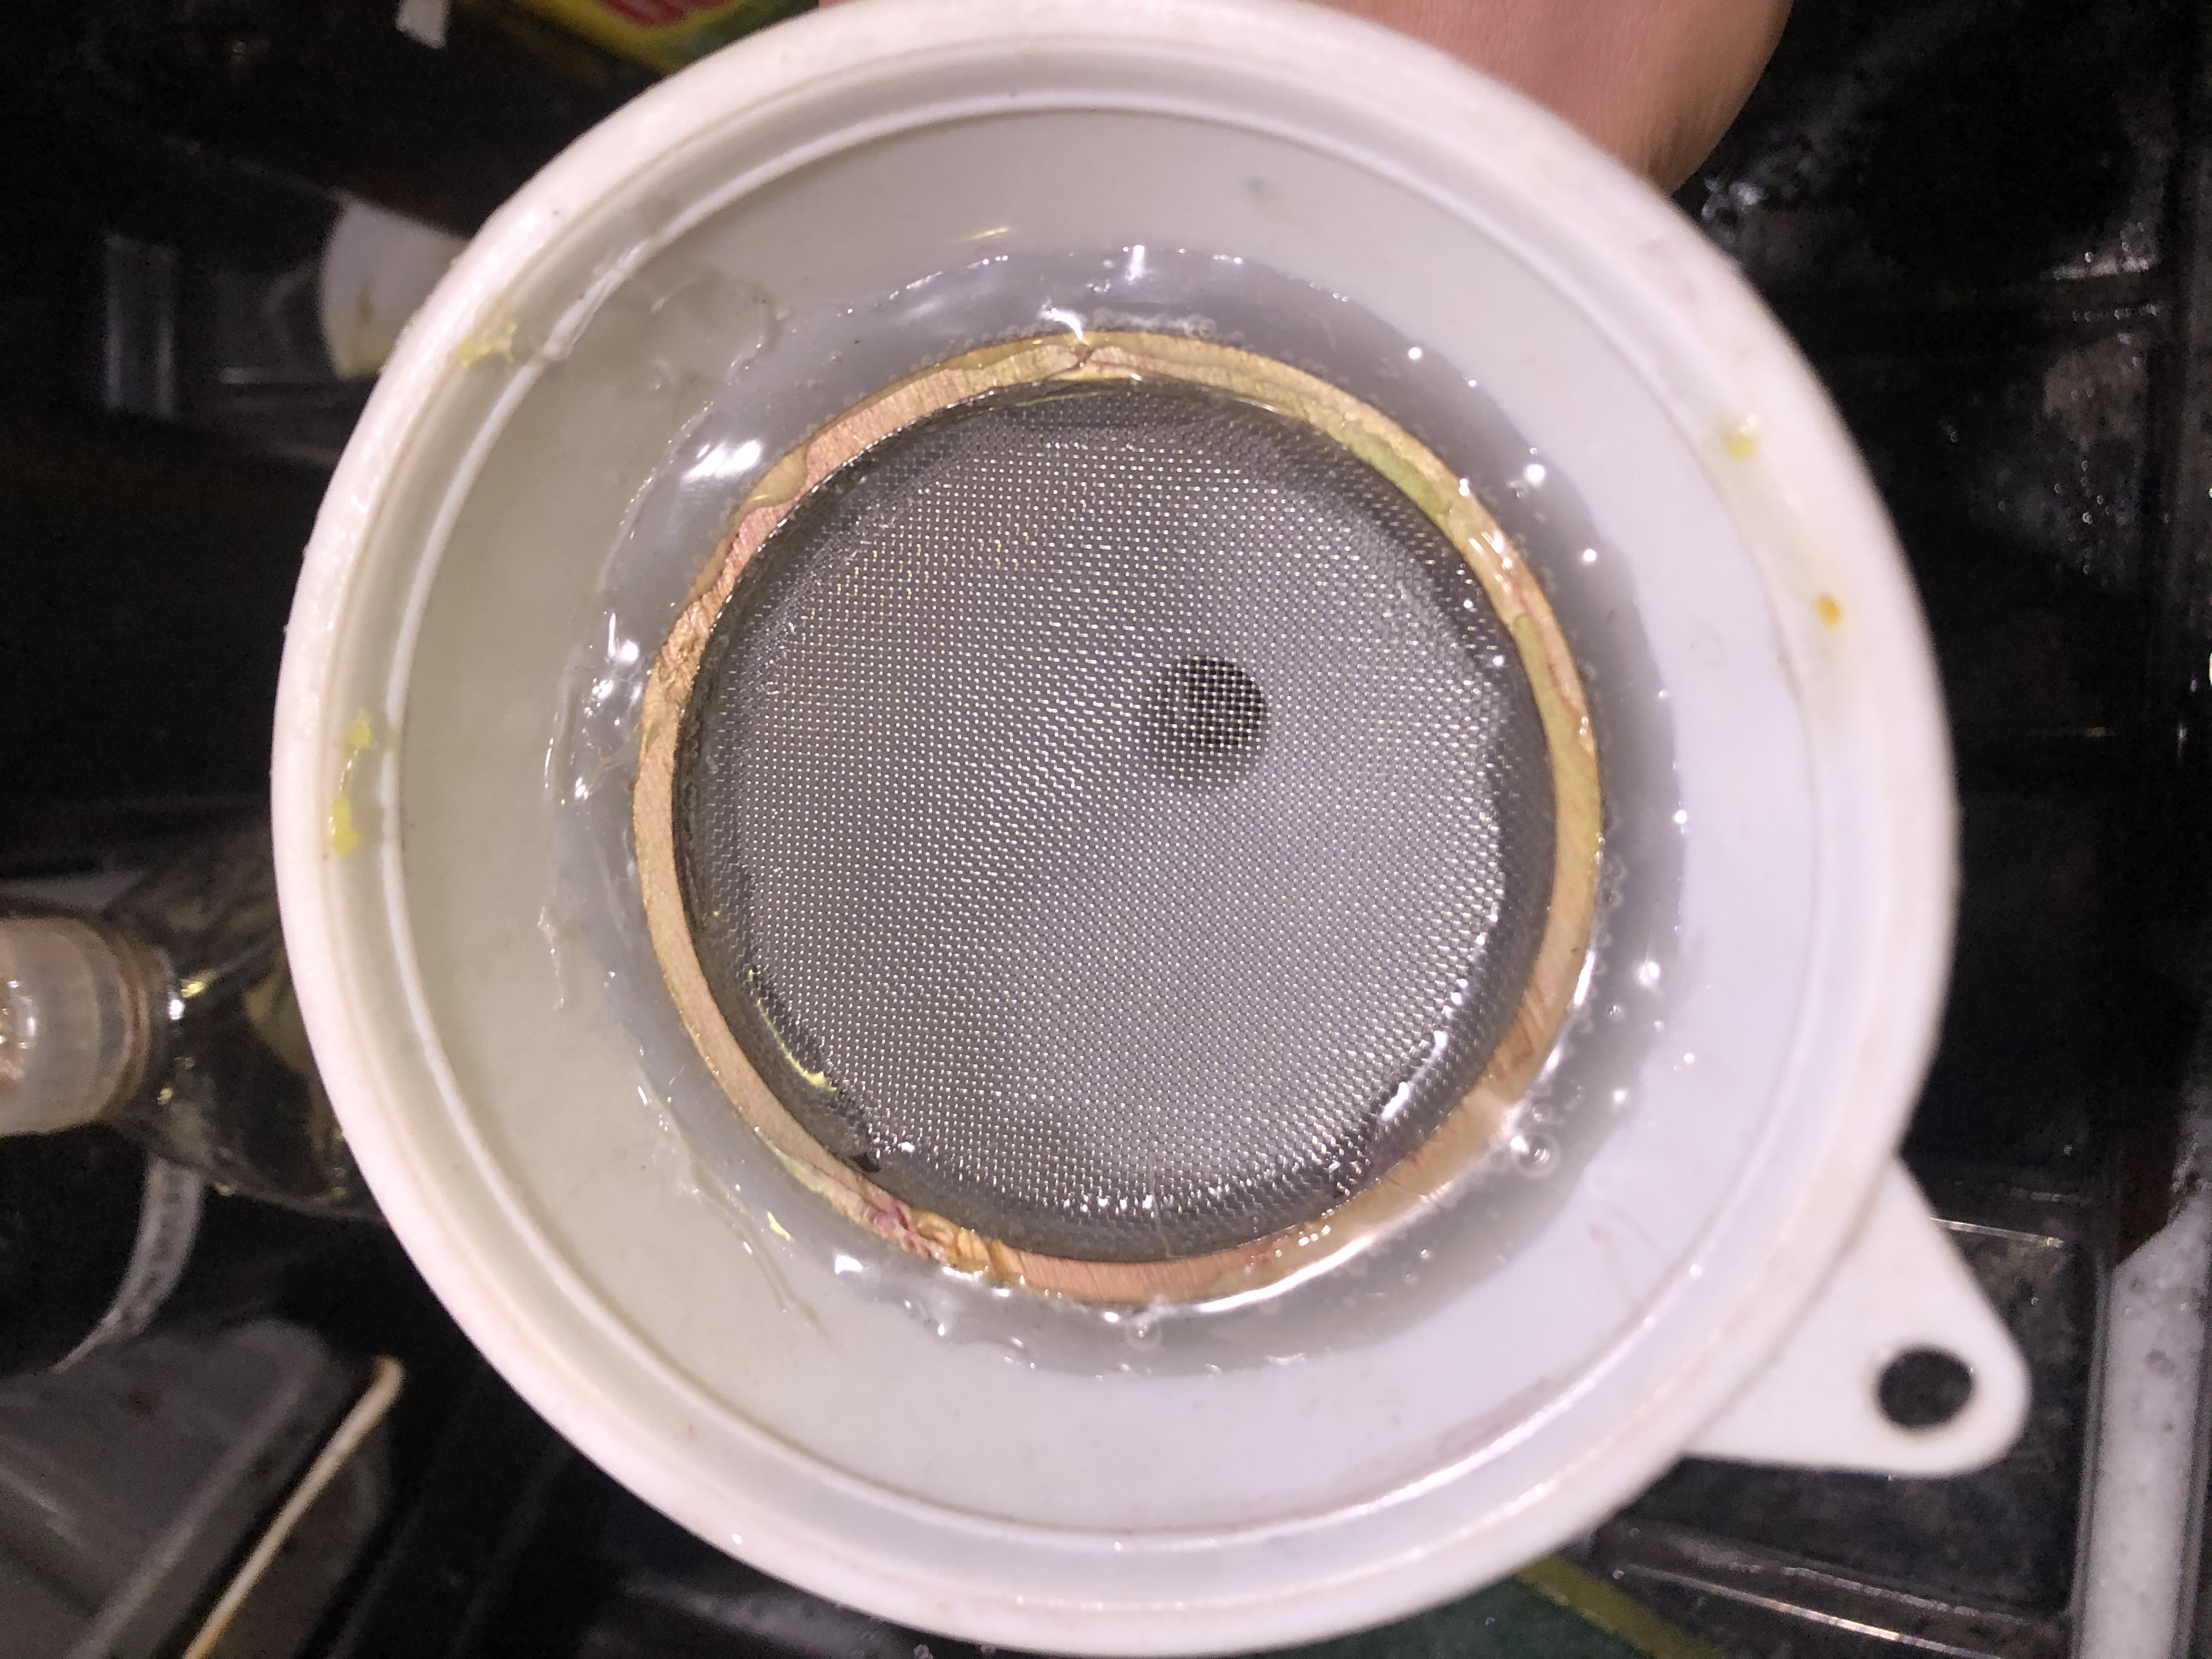
\includegraphics[width=3cm, height=3cm]{img/part1_12.jpg}
\end{center}

To unclump the starch a bit, I first add it to a mortar and pestle and mash it up. I then tip the contents through a filter strainer funnel I built. A lot of larger clumps won't pass through, but these can be forced through the mesh with the pestle. In general, this will break up the vast majority of the starch into a nice, smooth powder. In my experience, the green and violet starches don't need too much more work than this. If you experience more problems, \href{https://www.ebay.com/i/192595777161?chn=ps&var=492727707679&norover=1&mkevt=1&mkrid=711-117182-37290-0&mkcid=2&itemid=492727707679_192595777161&targetid=595076263848&device=c&mktype=pla&googleloc=9017518&campaignid=6470474296&mkgroupid=76413868734&rlsatarget=aud-622524040958:pla-595076263848&abcId=1140476&merchantid=6296724&gclid=CjwKCAiA__HvBRACEiwAbViuU09ehml6cnzs9T5qfvSzJk5uni9c-r_RrP4ihTn8yZGbFzYJMfQEphoCJ8kQAvD_BwE}{finer filters can be bought cheaply off of eBay}. I personally will strain any larger chunks through the 120 micron filter, returning what doesn't pass back to the mortar and pestle to be ground up more finely. If you're using sorted starch, I would strain everything again through a 53 micron strainer as well.\newline

Ultimately with the red starch, I find that there are still clumps that just won't break down, maybe around 10\% or so. Honestly, I just toss it at this point, as it's more trouble to deal with than it's worth.\newline

%link to video

Allow the three sets of dyes to dry completely for a day or two. Next, we are going to want to remove excess dye from the surfaces of the particles. If you skip this, dyes from each color may transfer to other colored particles, muddying the colors. Through experimentation, I've found that normal denatured alcohol from the hardware store does not penetrate into the starch grain. In a similar manner as before, add the colored starch to a 500mL beaker and fill it with the denatured alcohol. I prefer to magnetically mix for 30 - 60 minutes, before vacuum filtering the alcohol off and allowing the starch to dry. Dispose of the alcohol. Repeat a few more times for each color until the alcohol wash is mostly clear.\newline

\begin{center}
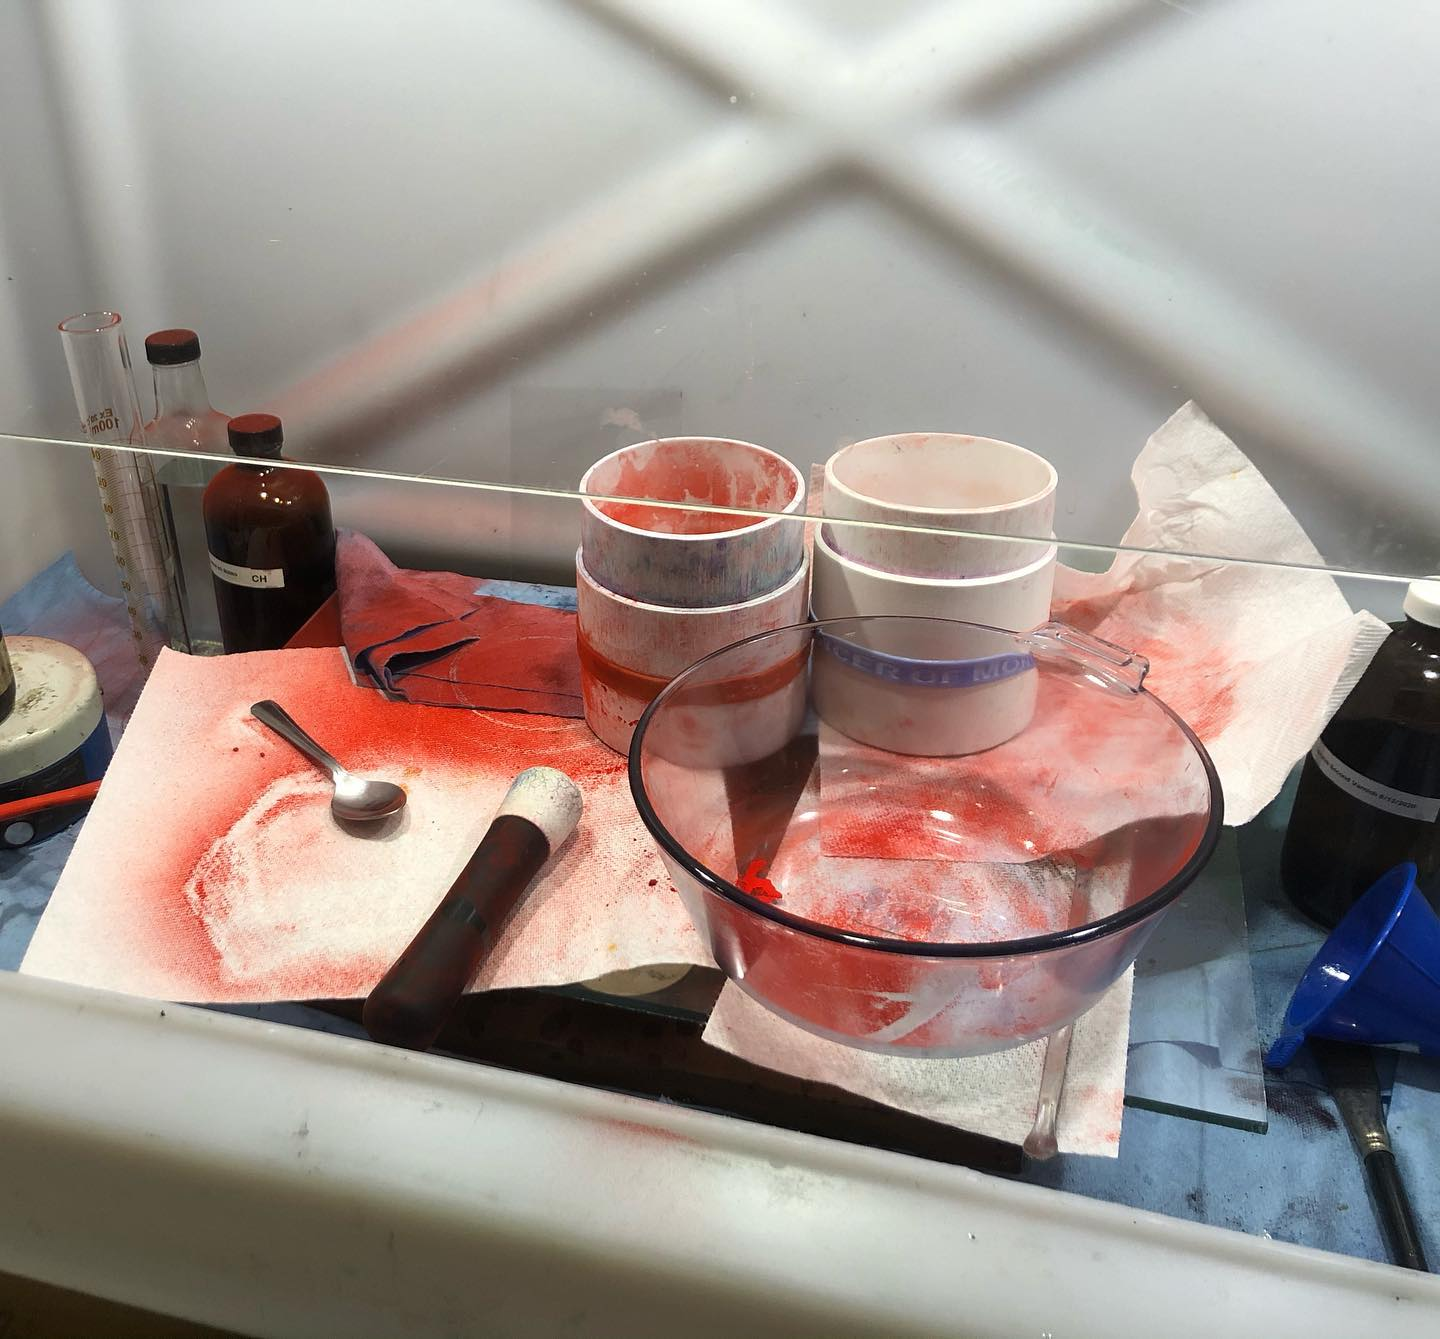
\includegraphics[width=5cm, height=5cm]{img/part1_13.jpg}
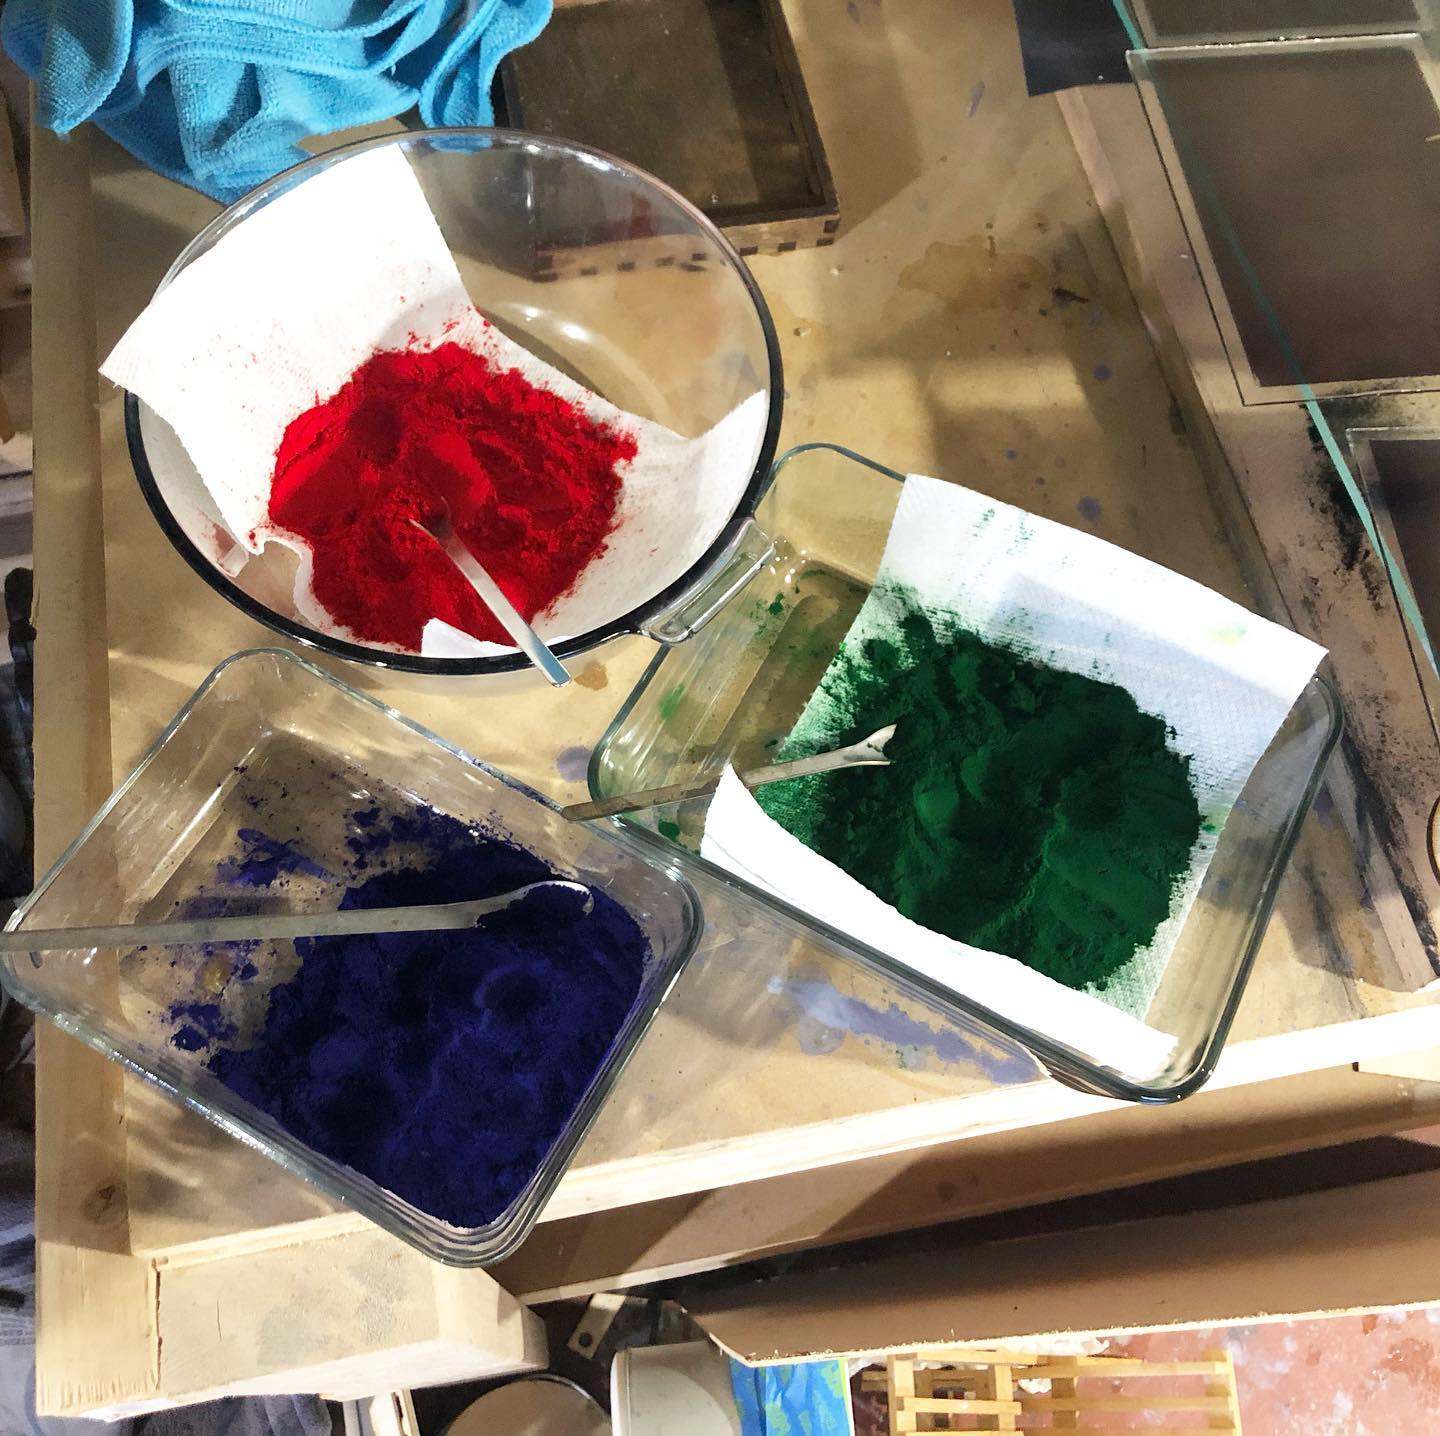
\includegraphics[width=5cm, height=5cm]{img/part1_14.jpg}
\end{center}

\subsection{The First Varnish}

We can now mix the "First Varnish". It's a thin, optically clear layer that adheres to the glass plate. It provides a tacky surface that the starch will readily stick to when gently dusted on.\newline

Traditionally, the Lumières dissolved natural rubber in toluene, with a little bit of waxy damar beta-resene. I struggled trying to source for raw latex that would dissolve, even going as far as to try out unlubricated condoms. Nothing seemed to work out. Fortunately, we have a very effective alternative that is stocked in nearly every local hardware store -- rubber cement! I weighed out, dried, and weighed again a portion of rubber cement to determine roughly how much rubber it contained. The rubber cement is then diluted with xylene (toluene will work just fine too if you have some on hand) to match the proportions of the original Lumière varnish. You will note -- in my formula, there is no damar component. I'm not sure why this was added to the original varnish, but I found that it had a tendency to reduce the tackiness of the plate, rather than enhancing it. The formula I still use is as follows:\newline
 
\textbf{The First Varnish}
\begin{itemize}
	\item Elmer's Rubber Cement, 32g
	\item Xylene, 200mL
\end{itemize}

Measure out the xylene into a 250mL beaker, and place on a magnetic mixer. Weigh out the rubber cement in a disposable weigh boat. While stirring, slowly tip the weigh boat and allow the rubber cement to flow into the beaker. Mix for another 5 minute or so, until the solution is clear and homogeneous. Gravity filter the solution through a coffee filter and bottle it. This stuff will last a real long time.\newline

Note: You're not going to get insta-cancer just by getting a whiff of it, but xylene/toluene fumes aren't great for you health either. Whenever working with the varnish, whether it's mixing it up or coating glass plates, you should probably be doing it either in a fume hood or outside.\newline

\subsection{Mixing and Dusting the Starch}

We have our three portions of starch, now we need to mix them together correctly to form a neutral-colored screen! One might think that this is as simple as weighing out the same amount of each color, but unfortunately it's not quite that straightforward. The same mass of starch of each color may not correlate to the number of grains anymore, since the different dyes have different densities. Also, different colors may transmit more or less light than the other two. For this reason, the only practical way to mix the starch is by trial and error, and heavy emphasis on taking notes.\newline

Firstly, let's coat a glass plate with the first varnish. This will give us a substrate on which to dust the starch we're testing. With the glass plate in one hand and the bottle in the other, pour an amount of the varnish onto the center of the glass. Gently rock the plate around, so that the varnish covers the whole surface. When done, tip the corner of the plate and let the excess run back into the bottle. Set the plate down on a level surface and allow an hour or so for it to be completely dry -- if you can still smell the xylene, it's not dry yet!\newline

While you're waiting on this, measure out 2g of each color of starch into a beaker (or whatever other container), and mix it around with a small spoon or spatula. Eventually the individual colors will disappear, and the mix should take on a dark red appearance. You can't overmix, so be thorough here!\newline 

When the plate has dried, scoop a dime-sized amount of starch onto the plate, and spread it around a bit with a soft paint brush to about the size of a quarter. Brush the extra back into your starch container. There will be a lot of interstitial space between the grains, so to get a proper idea of the color balance we're going to need to crush it. This can be done a few ways:\newline

1. Take a spoon and just kind of roll it around for a few seconds. You should notice the smushed starch visually darken a bit, and become a bit more shiny.\newline

2. My preferred method is to take a 1" castor transfer ball (\href{https://www.amazon.com/DGQ-Transfers-Furniture-Trolley-Mounted/dp/B07HC3Z56Z/ref=sr_1_10?dchild=1&keywords=1%22+caster&qid=1587136812&sr=8-10}{like these lil duders here}) and roll it around in a few small circles while applying a downward pressure. You might want to try and wipe some of the oil off of the ball first, as it'll soak into the starch a bit (it's not a huge deal though).\newline

After a small section has been crushed, observe it against a nice cool light, phone screen, or diffuse sun on a white object. You should notice a color cast. From here, you will have to determine what color to add and start the process over. Try adding 0.5g of whatever corrective color needs to be added, remix, and flatten again. This can take several tries until the screen becomes close to neutral. Don't get impatient, but don't panic if it's not perfectly neutral either. Each batch of screens I've made always have a slight color bias, and this can be corrected for later. Keep track of the additions, and once you're happy with your color balance, scale it up to make about 50-100g of starch mix.\newline

With your full starch mix, I recommend washing them all together in alcohol one or two more times. As scary as this sounds, I've found that this gives you a nearly completely homogenous mixer, and the colors absolutely will not bleed into each other during the process. Mix as before, vacuum filtering the alcohol from the starch, and repeating until the runoff is fairly clear.\newline

\begin{center}
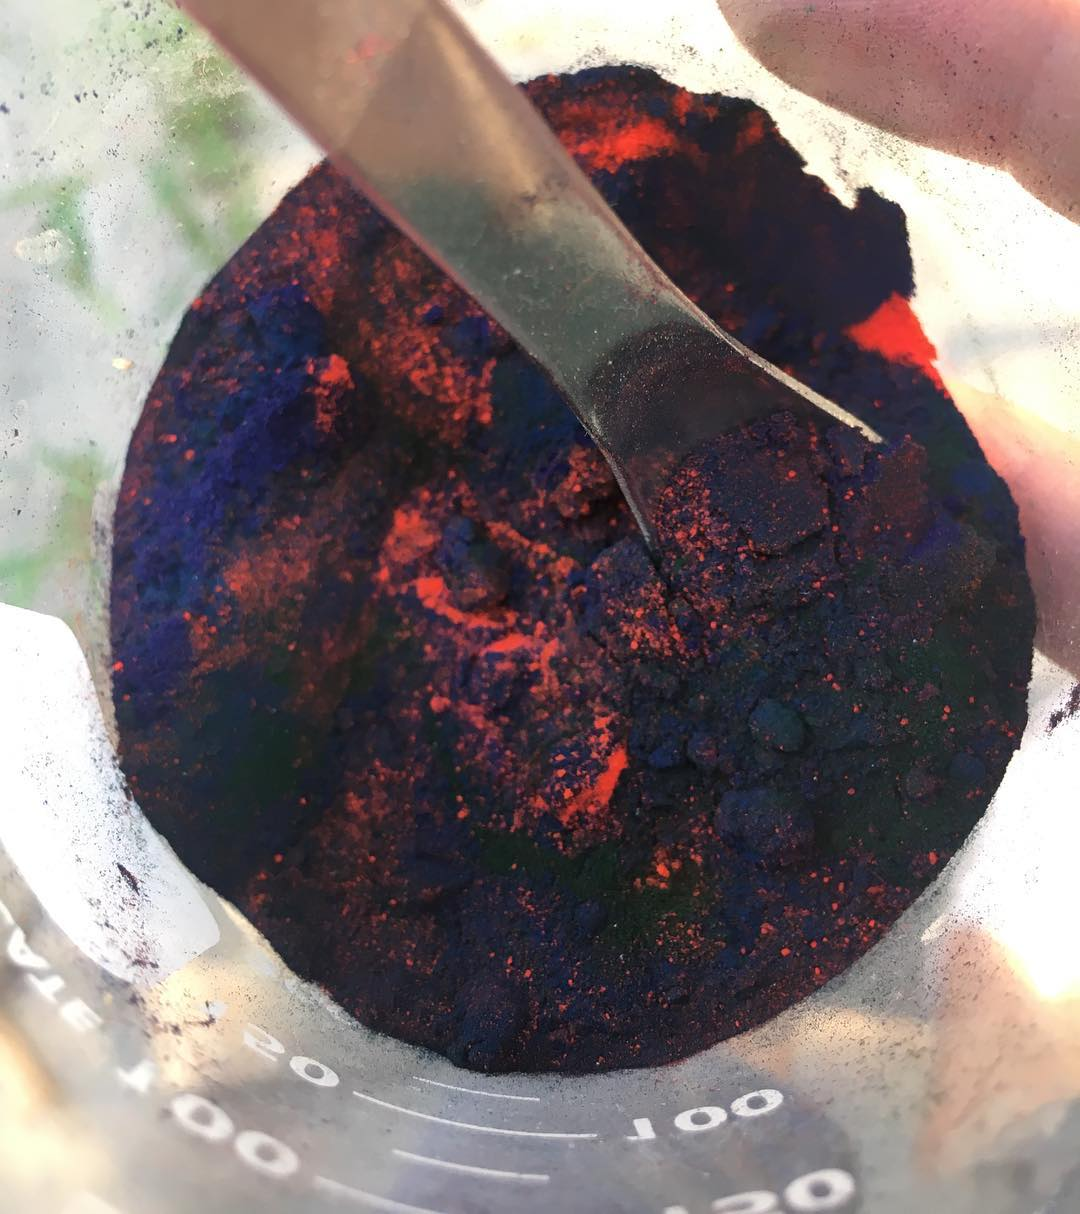
\includegraphics[width=5cm, height=5cm]{img/part1_15.jpg}
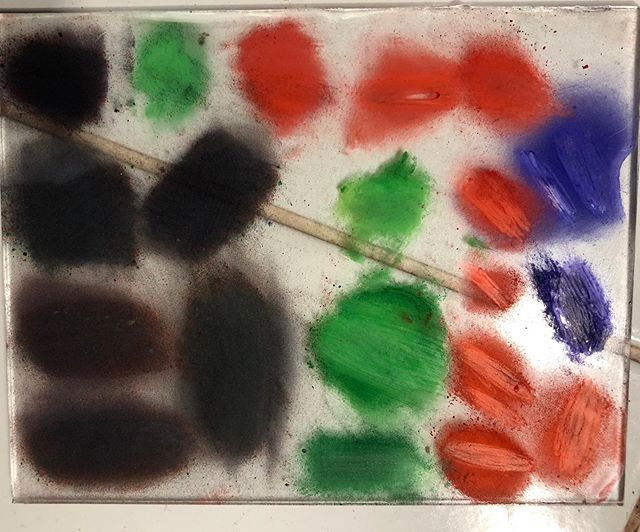
\includegraphics[width=5cm, height=5cm]{img/part1_16.jpg}
\end{center}

Now that we officially have our starch ready, we can begin to work on our first autochrome screen plates! First, pour on the first varnish we mixed up, rocking the plate for full coverage, and then pour the excess back into the bottle. Allow the plates to dry vertically for a few hours, until they no longer smell like toluene.\newline

I used to recommend masking the outer 1/4" with masking tape. My reasoning in the past was that it would prevent leaks from the sides by allowing the second varnish to fully envelope the plate. In practice, the second varnish had poor adhesion to the glass, and was more likely to flake, peel, and crack. Better just to cover the whole thing with starch.\newline

After they have dried, take a quarter-sized scoop of starch and plop it in the middle of the plate. Spread the starch around with a small paint brush until it has covered the whole plate. With a soft, long-haired makeup brush, gently brush the extra off the plate and back into the starch container. Now we should be ready for compression.\newline

\begin{center}
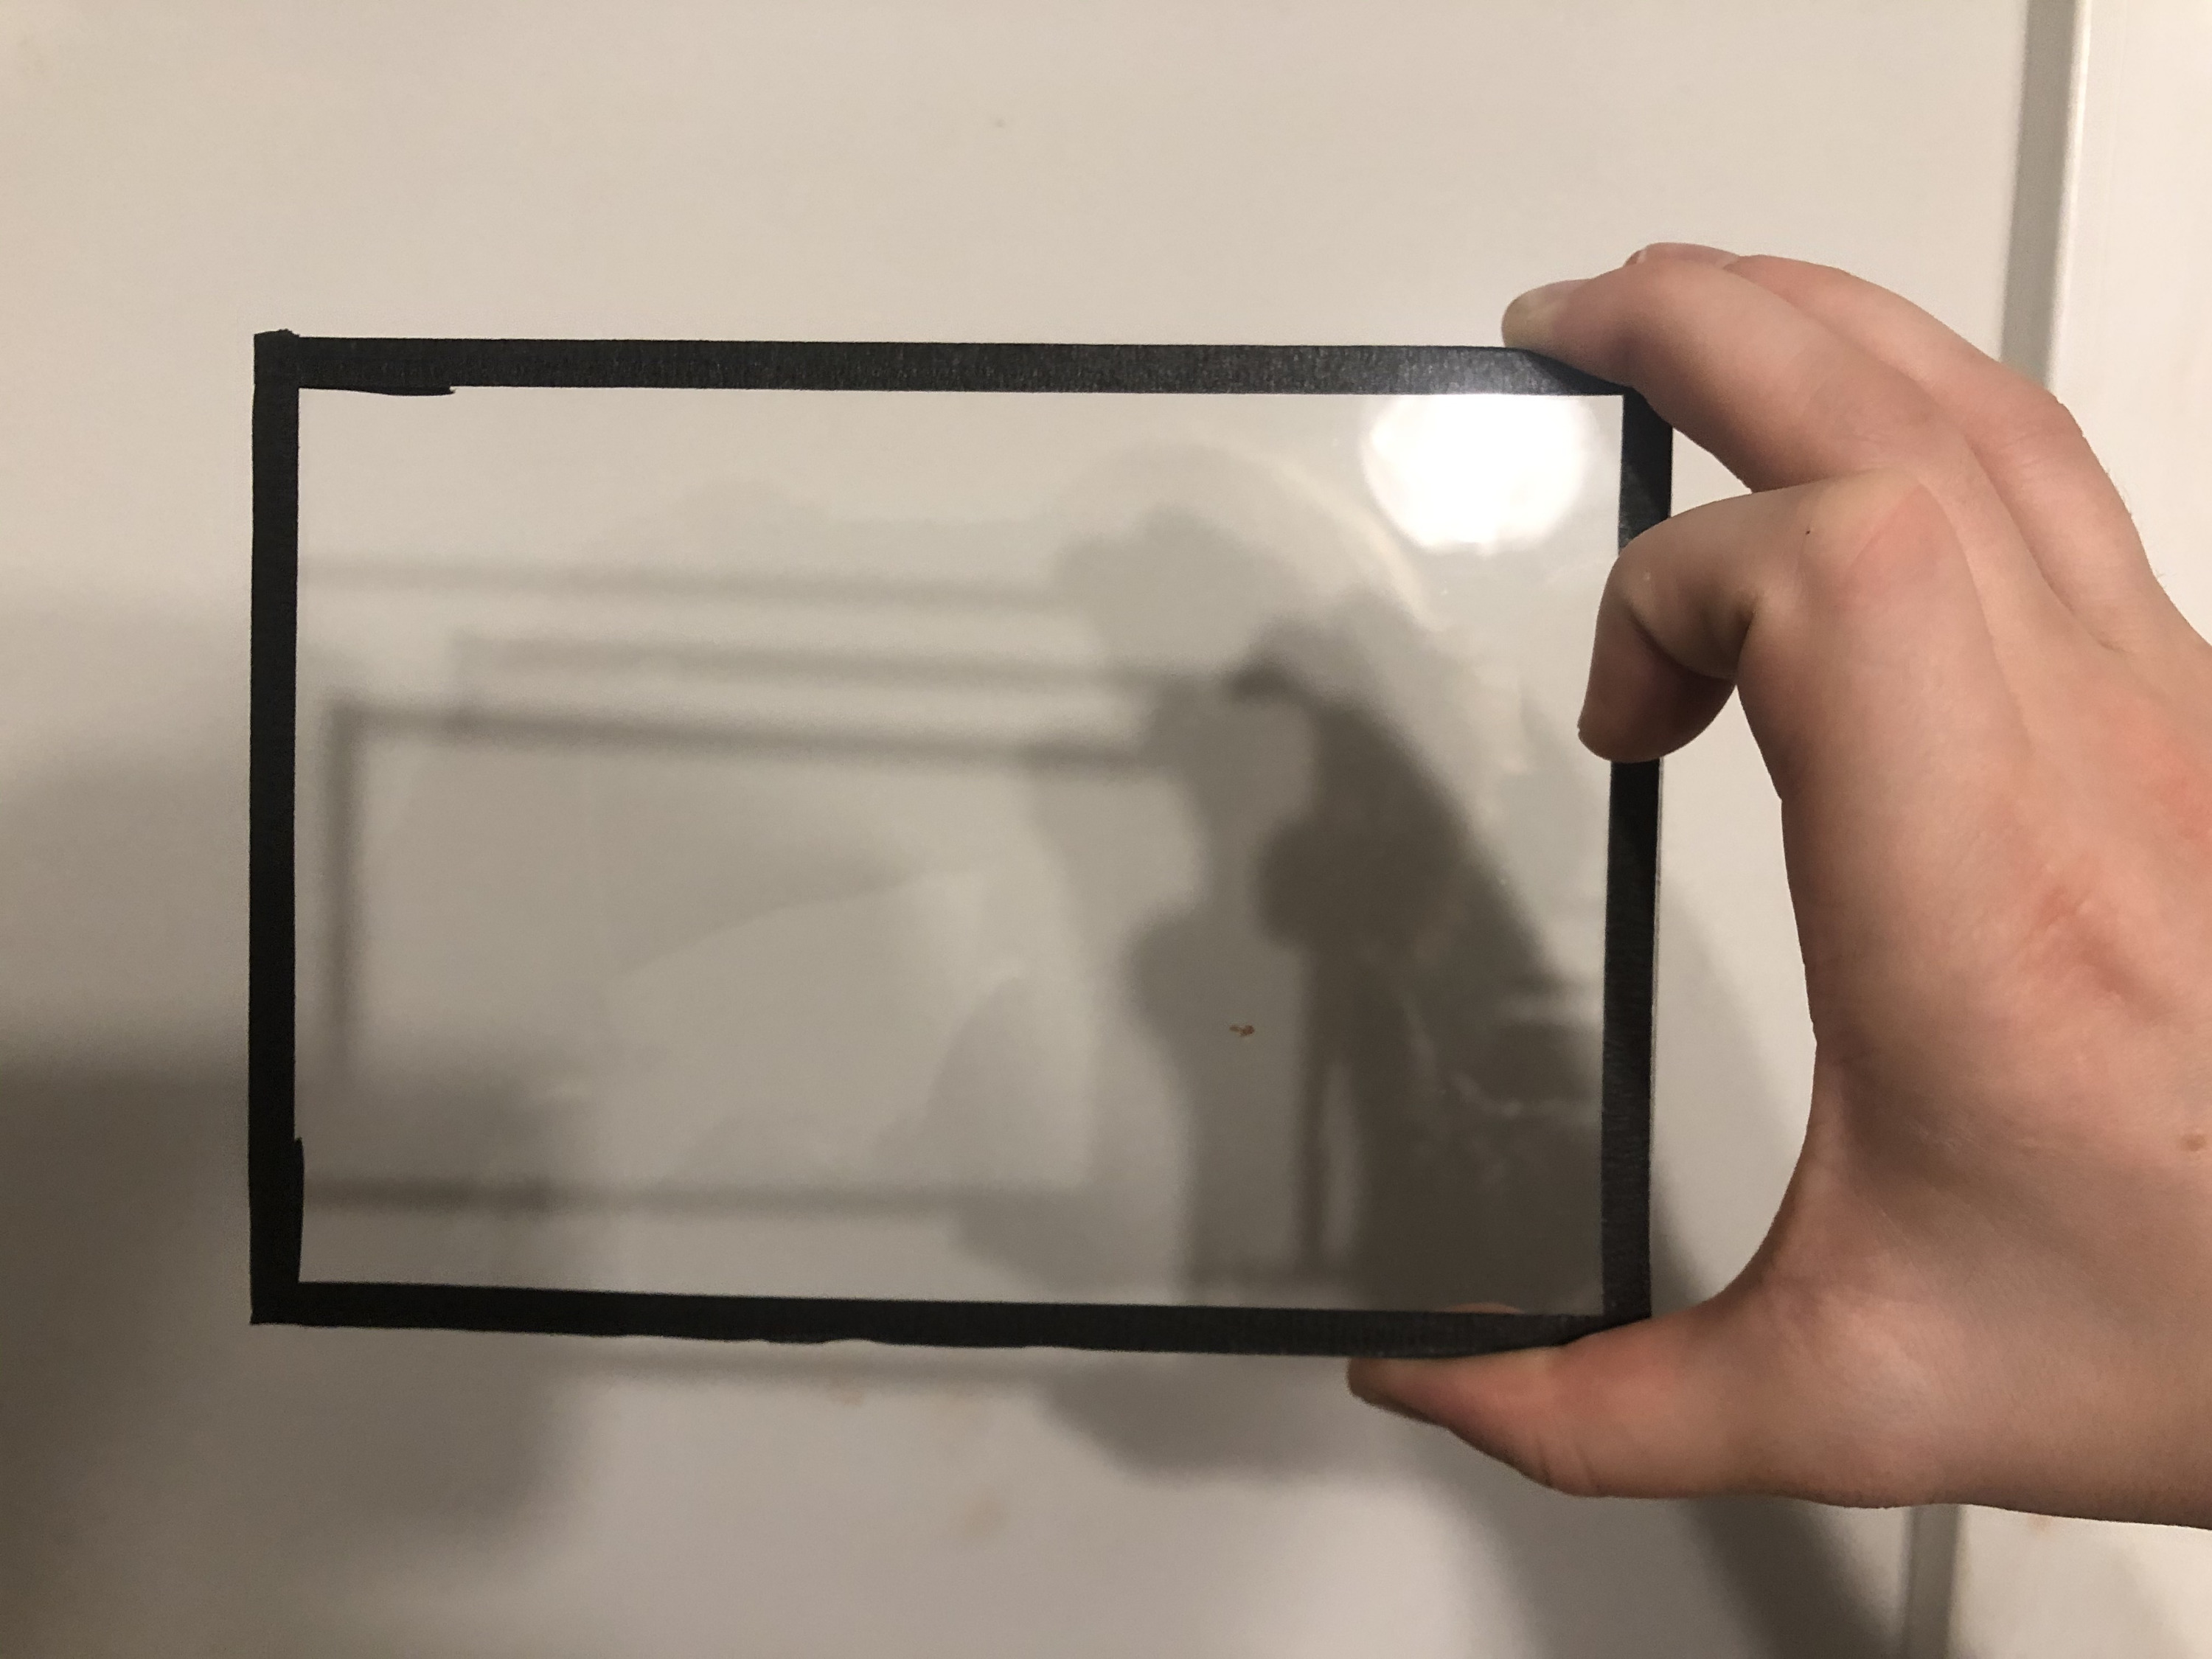
\includegraphics[width=5cm, height=5cm]{img/part1_17.jpg}
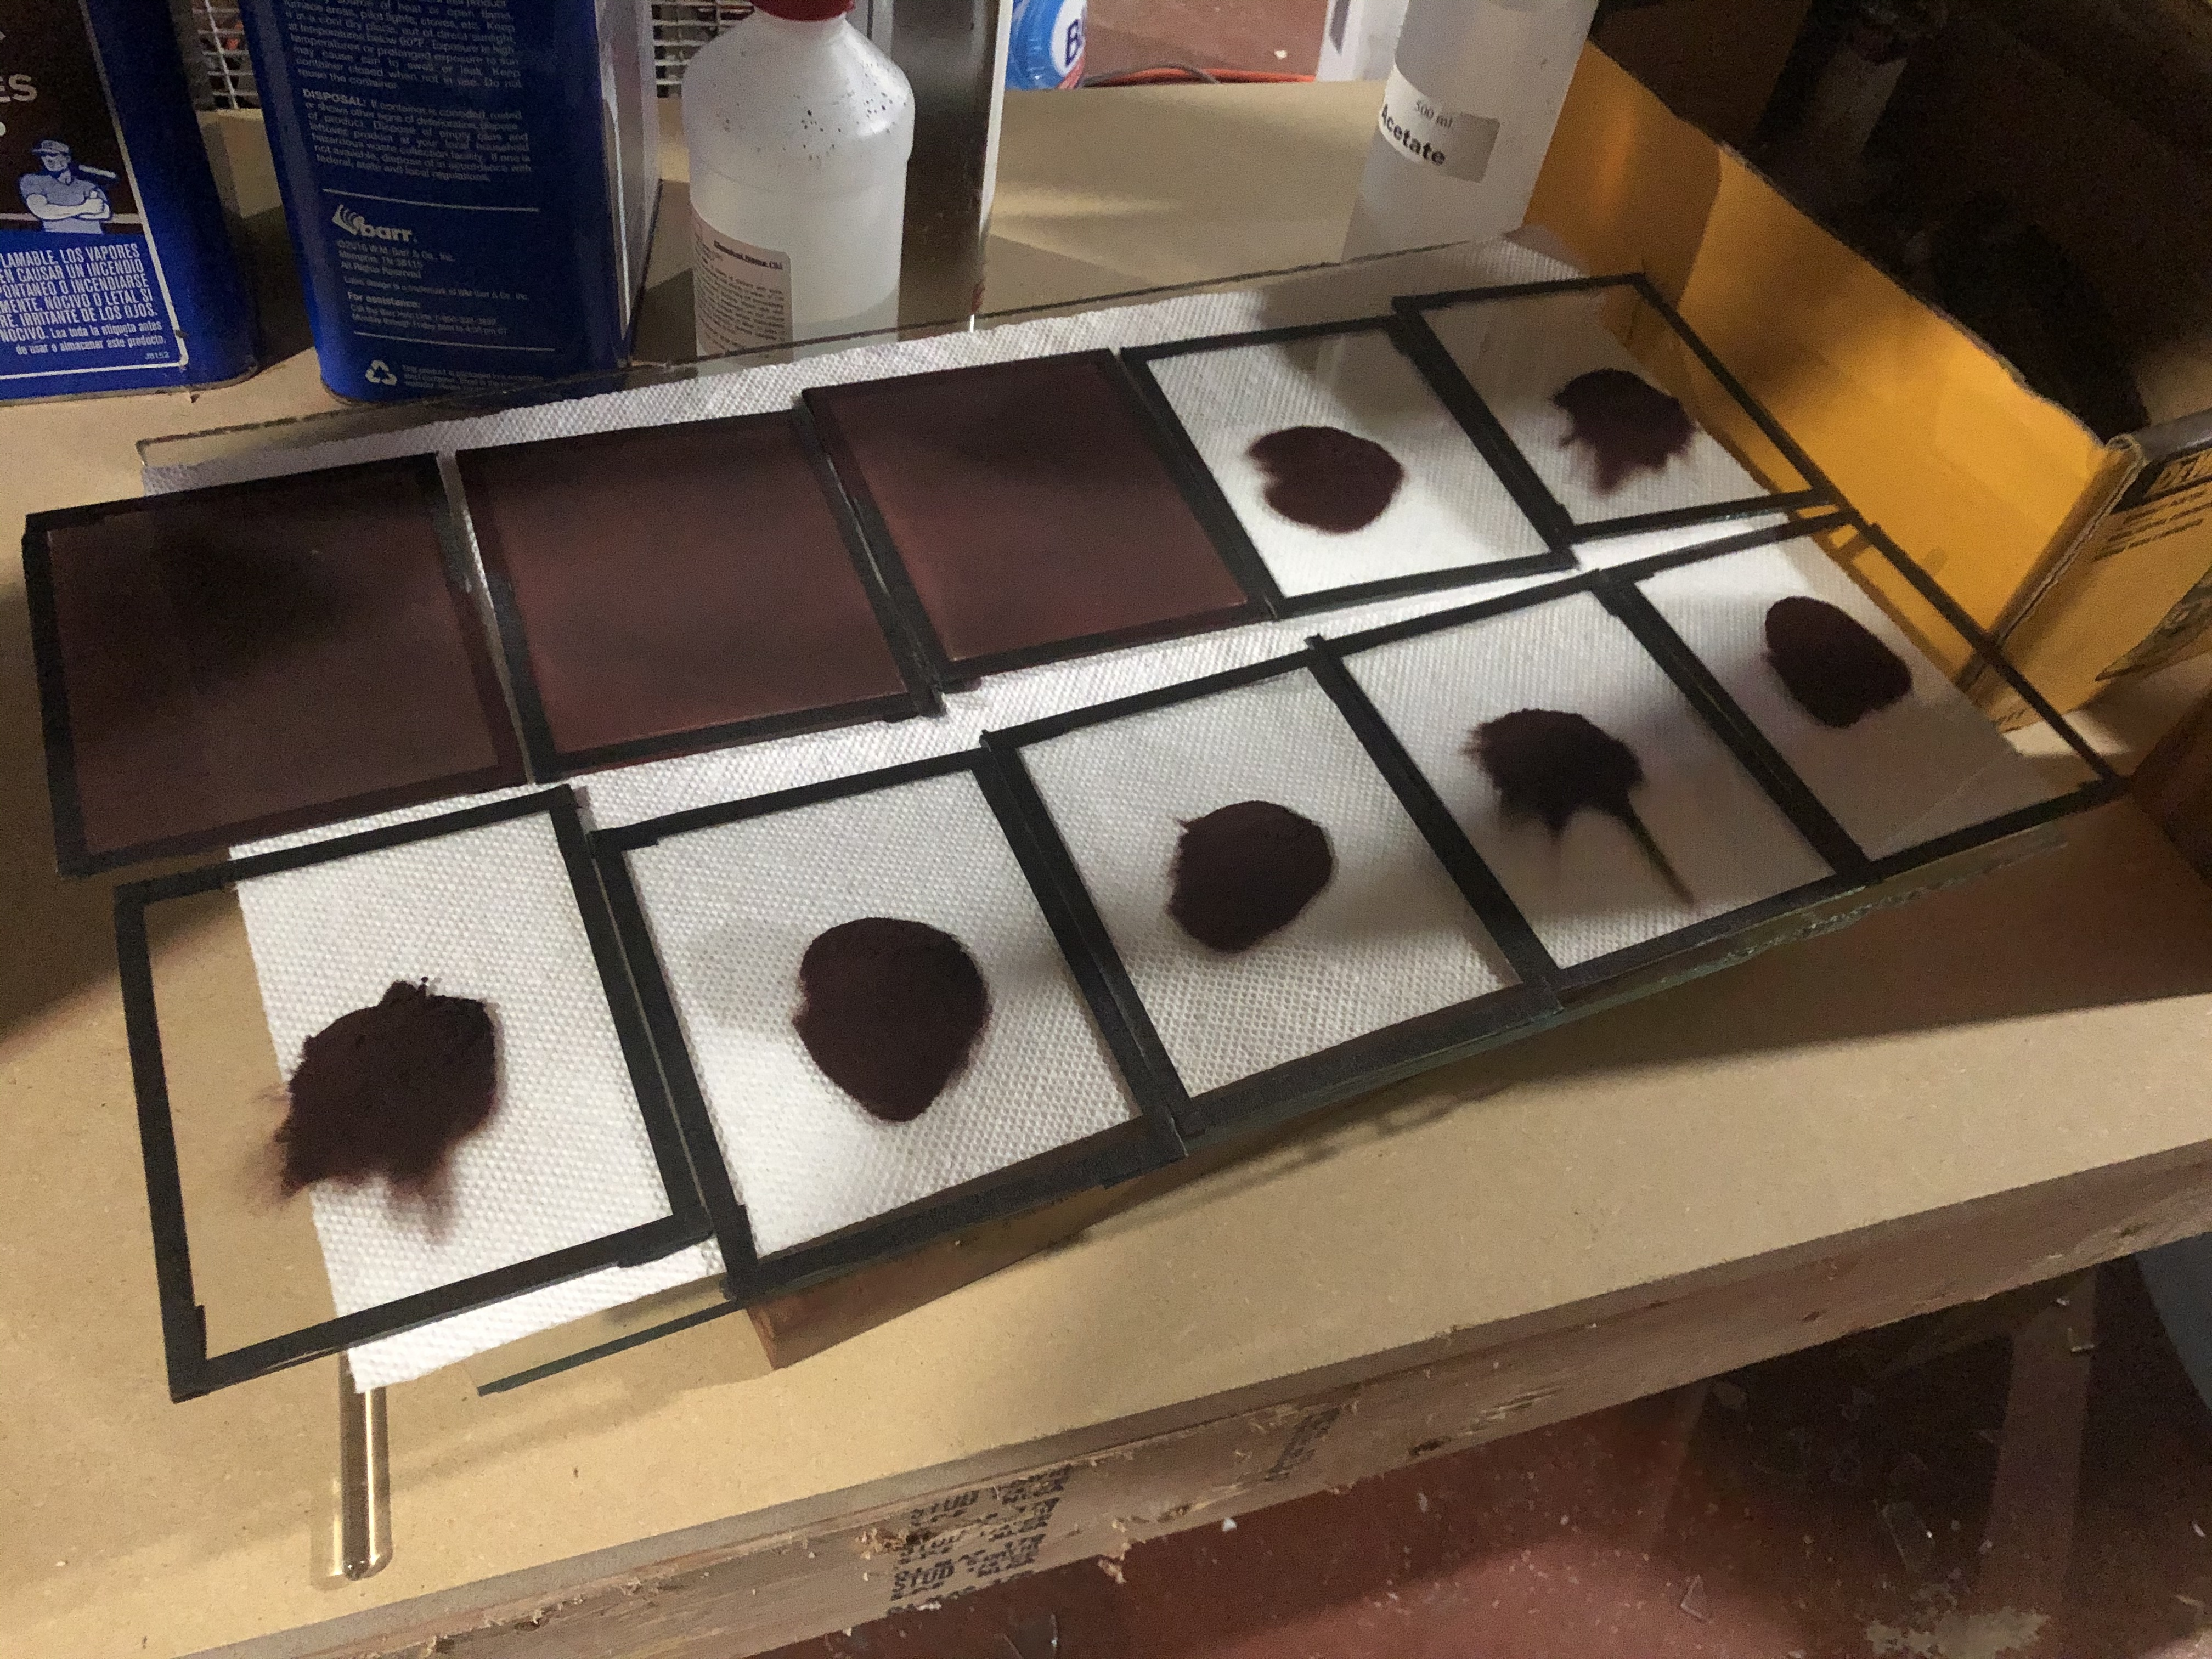
\includegraphics[width=5cm, height=5cm]{img/part1_18.jpg}
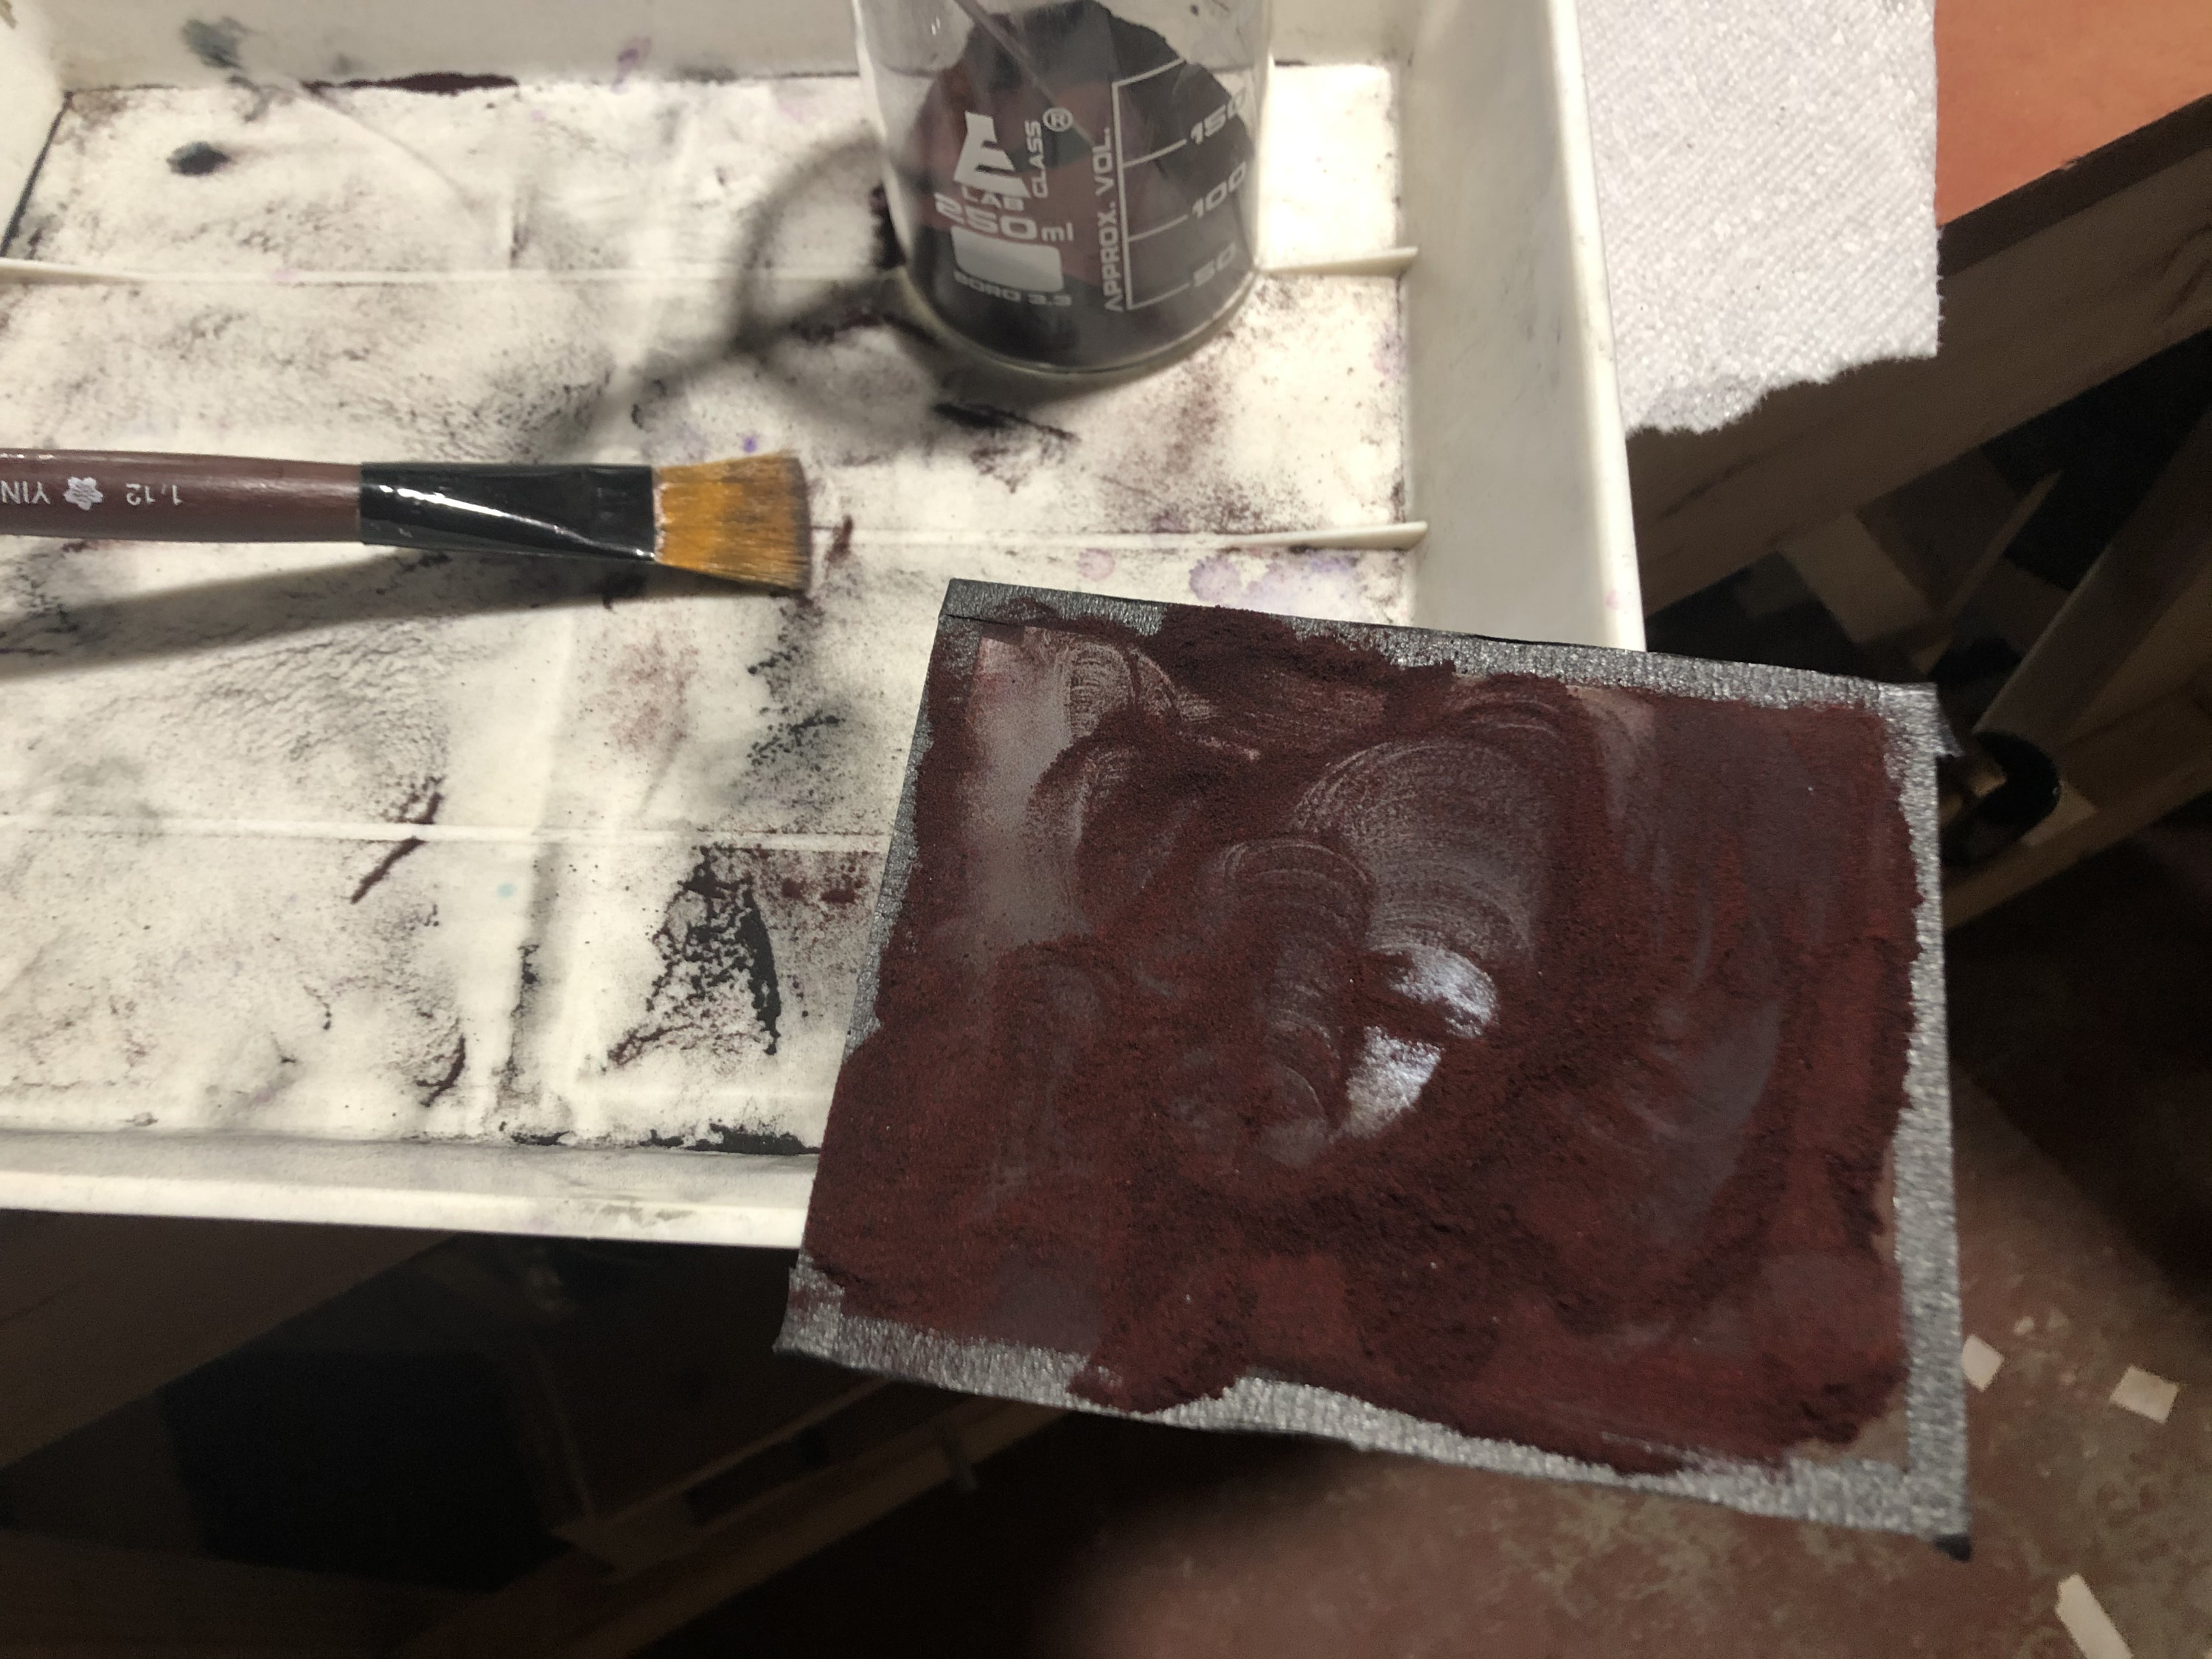
\includegraphics[width=5cm, height=5cm]{img/part1_19.jpg}
\end{center}

\subsection{Compressing the Starch}

The starch is now adhered to the sticky plate surface, but there is still quite a bit of interstitial space in between each grain. Not only will compression reduce this in-between space, it will also considerably improve the plate's overall transparency.\newline

\begin{center}
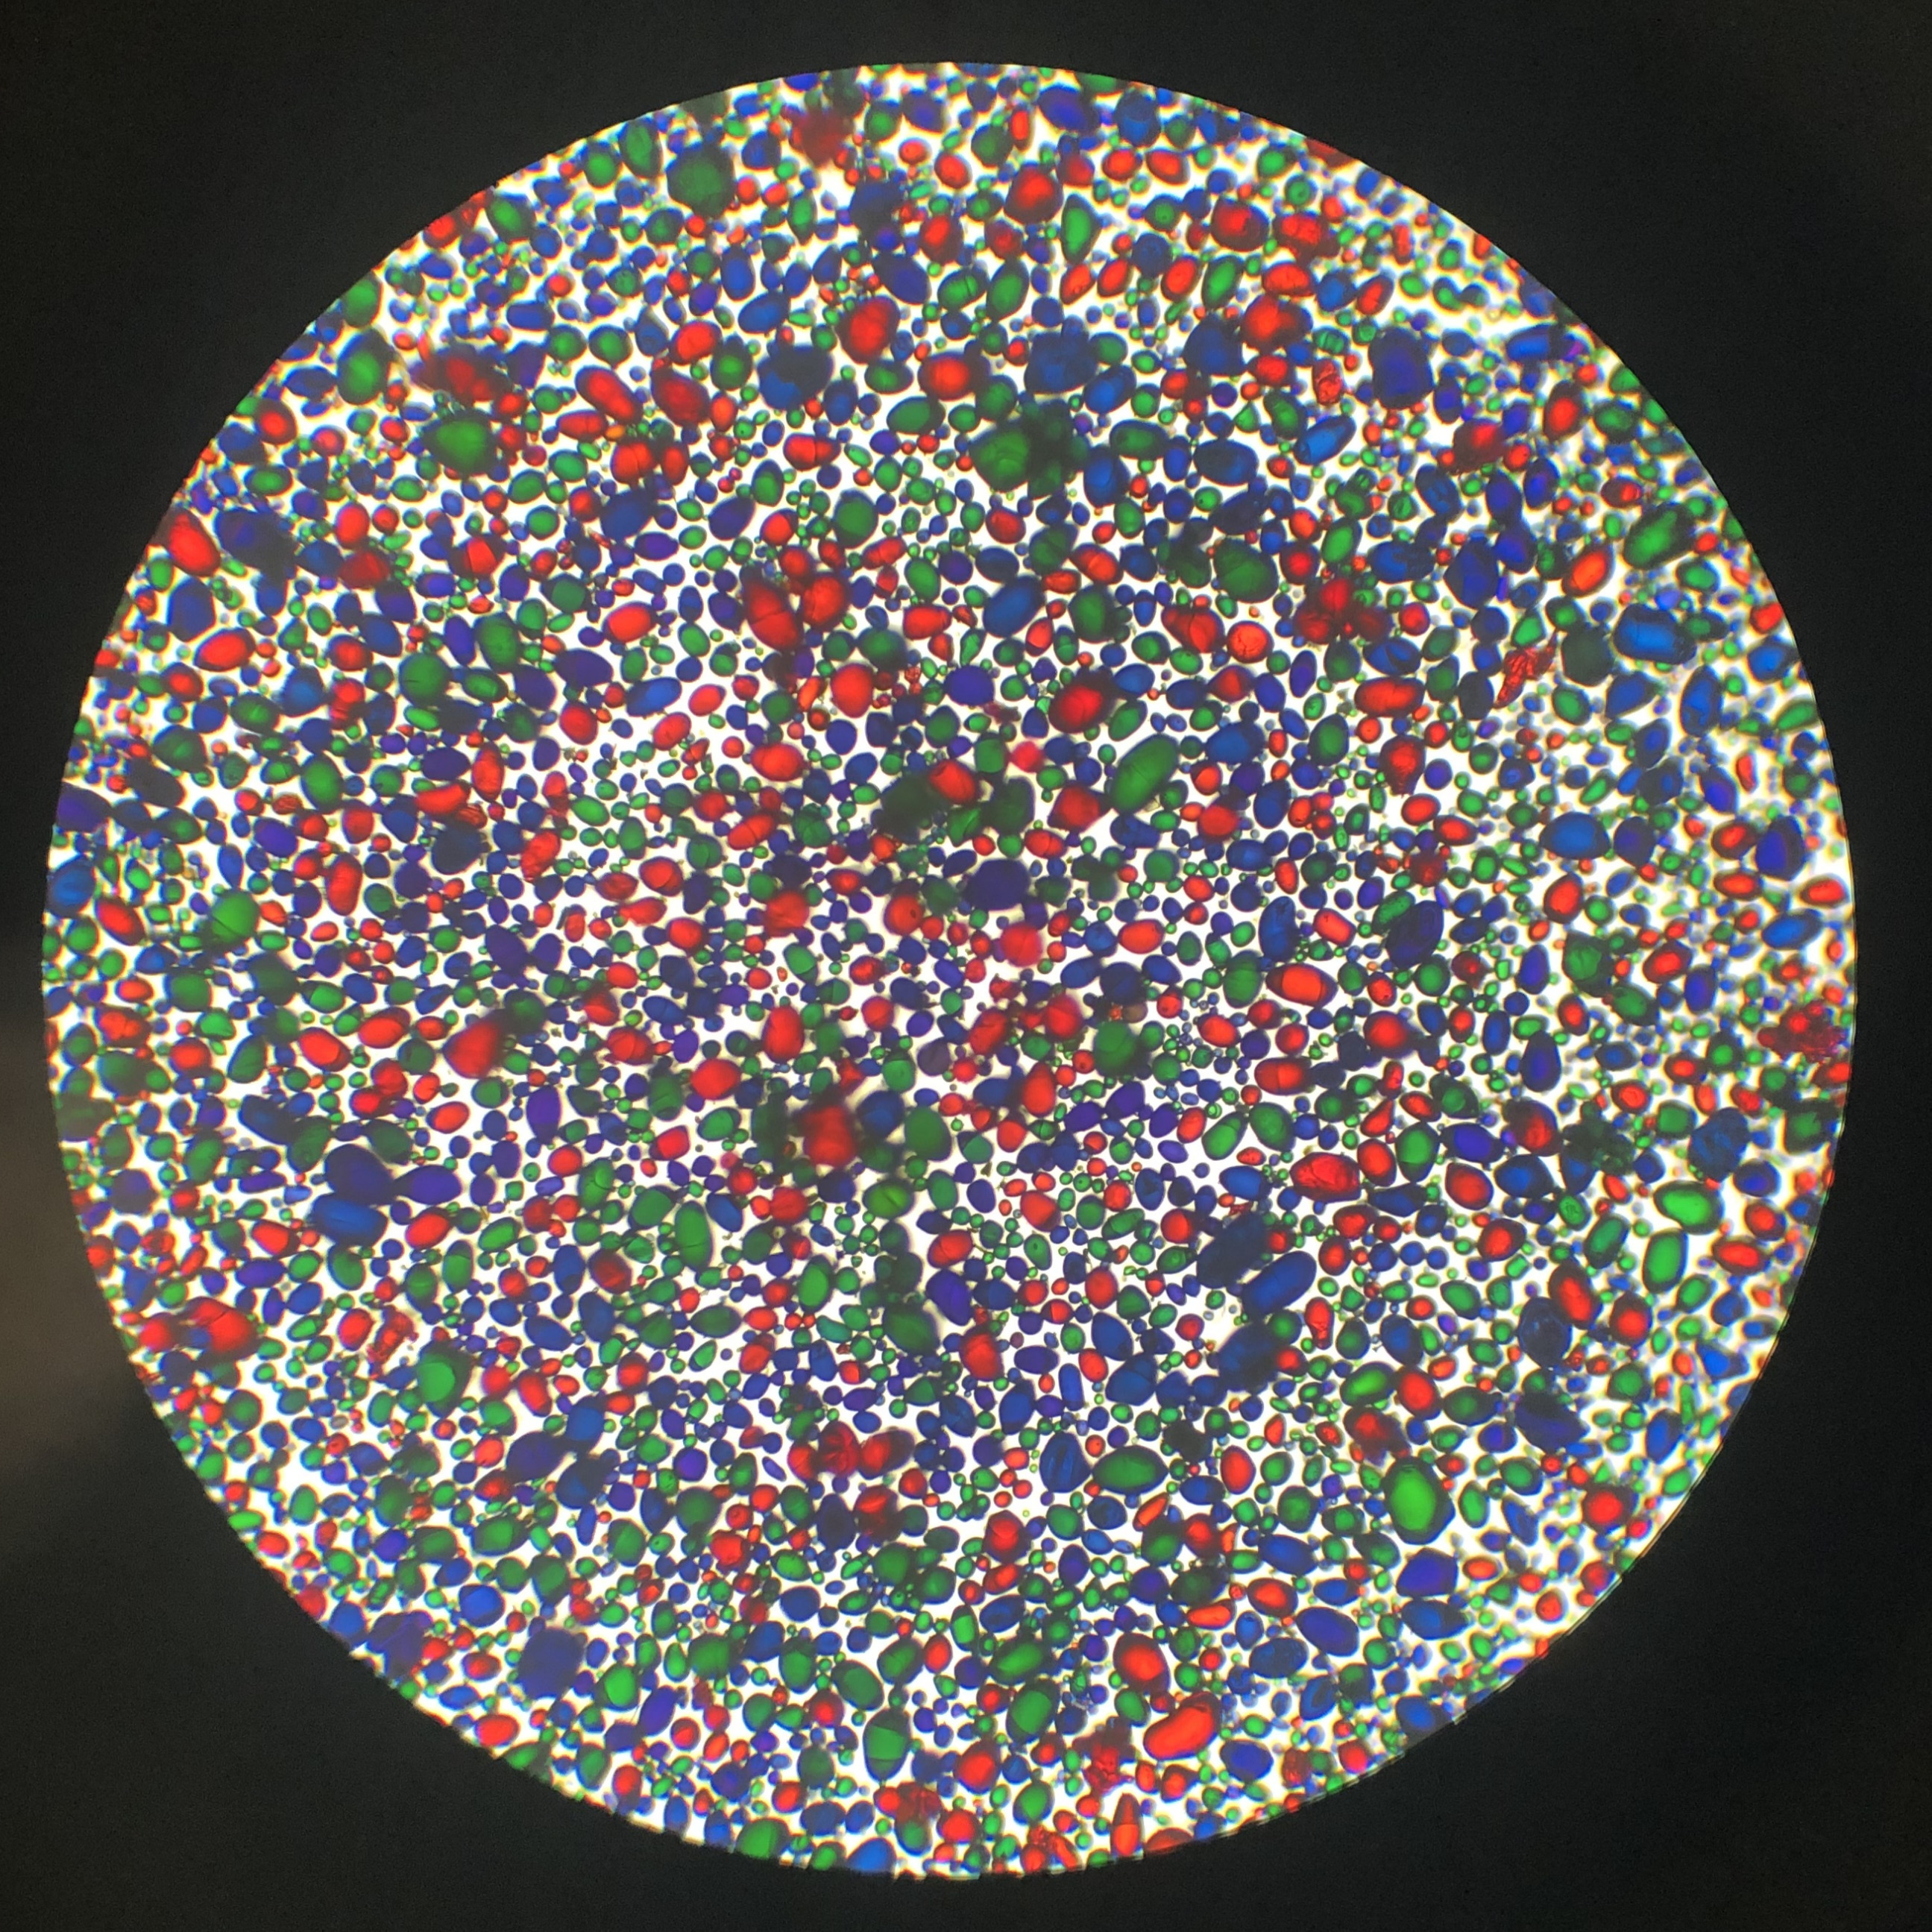
\includegraphics[width=4cm, height=4cm]{img/part1_20.jpg}
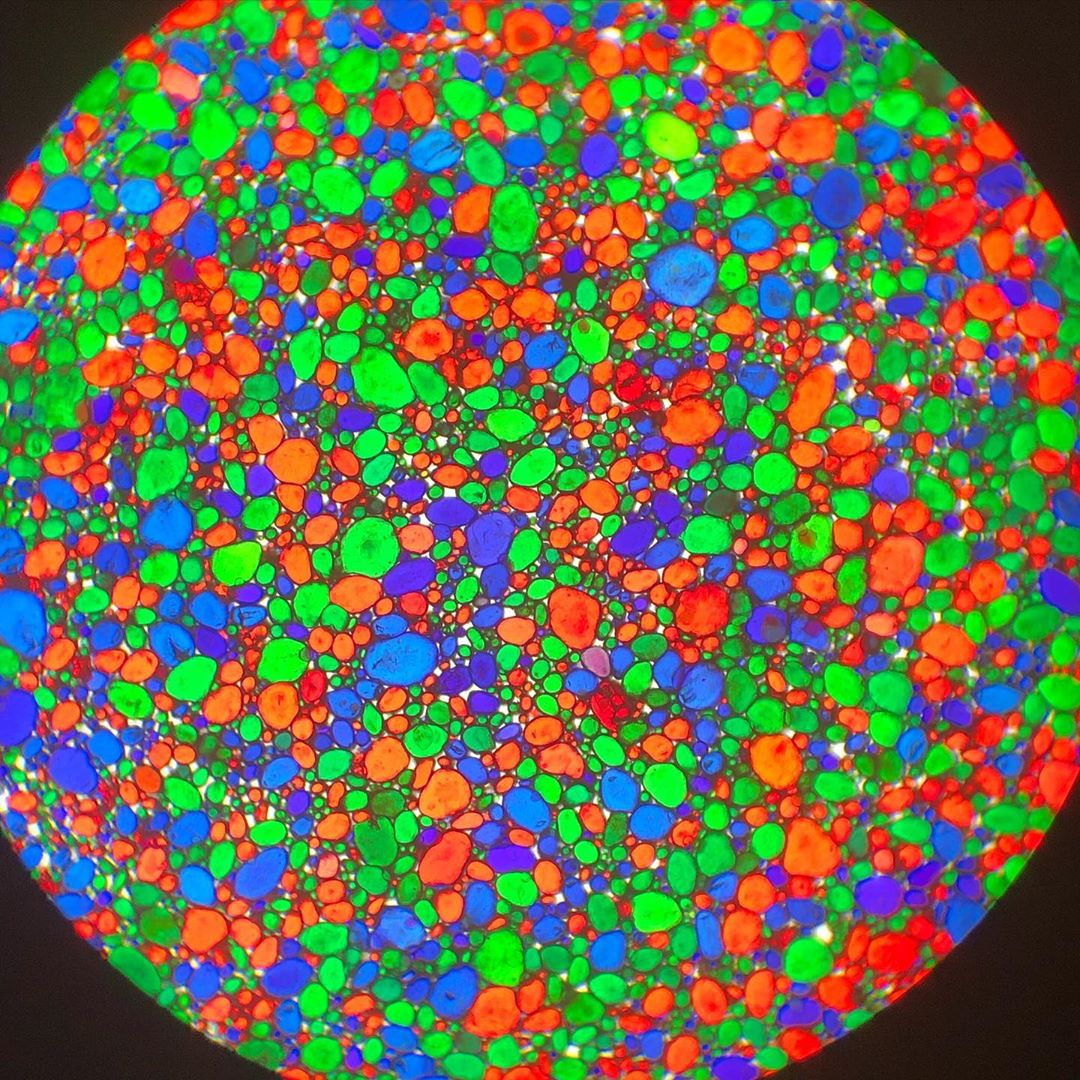
\includegraphics[width=4cm, height=4cm]{img/part1_21.jpg}
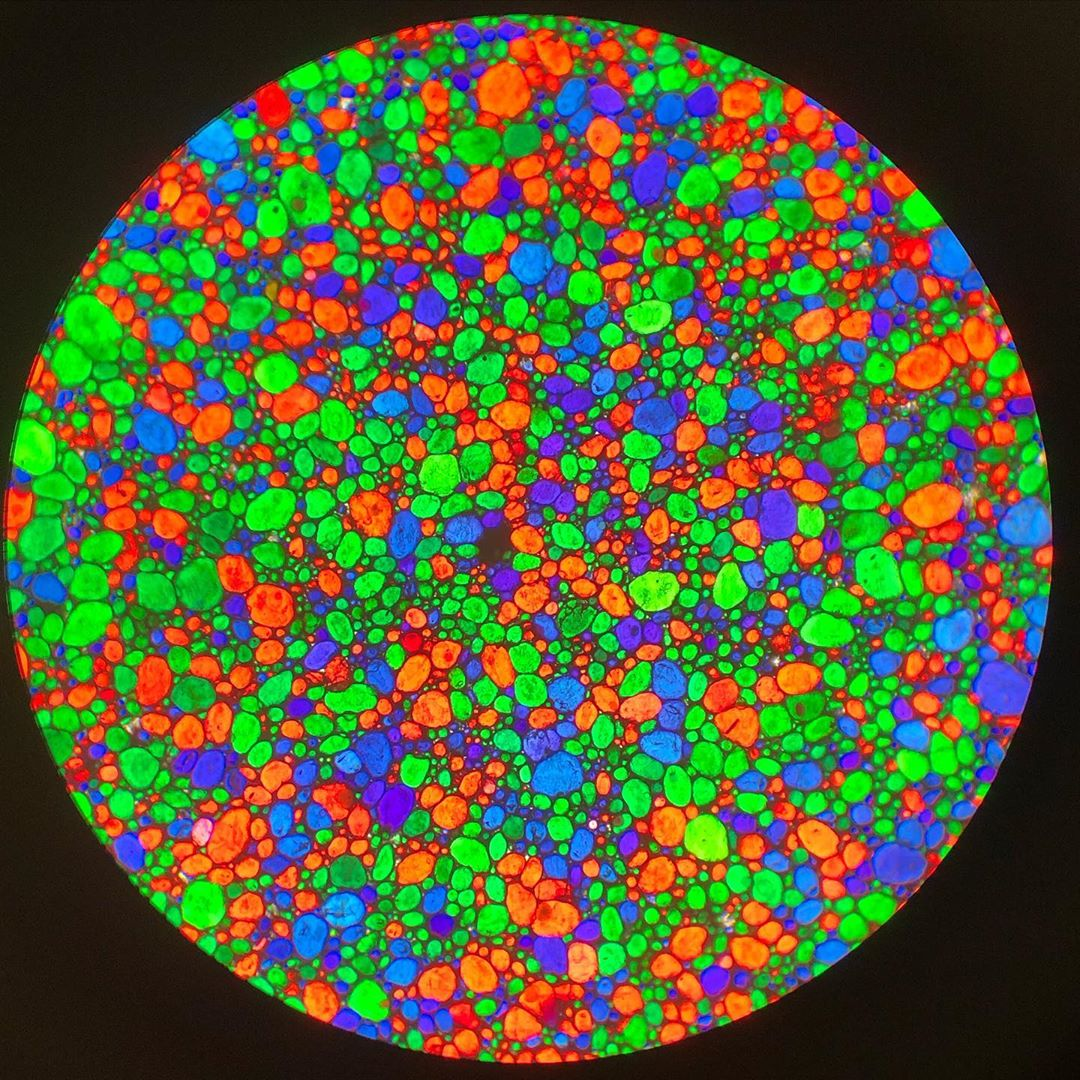
\includegraphics[width=4cm, height=4cm]{img/part1_22.jpg}
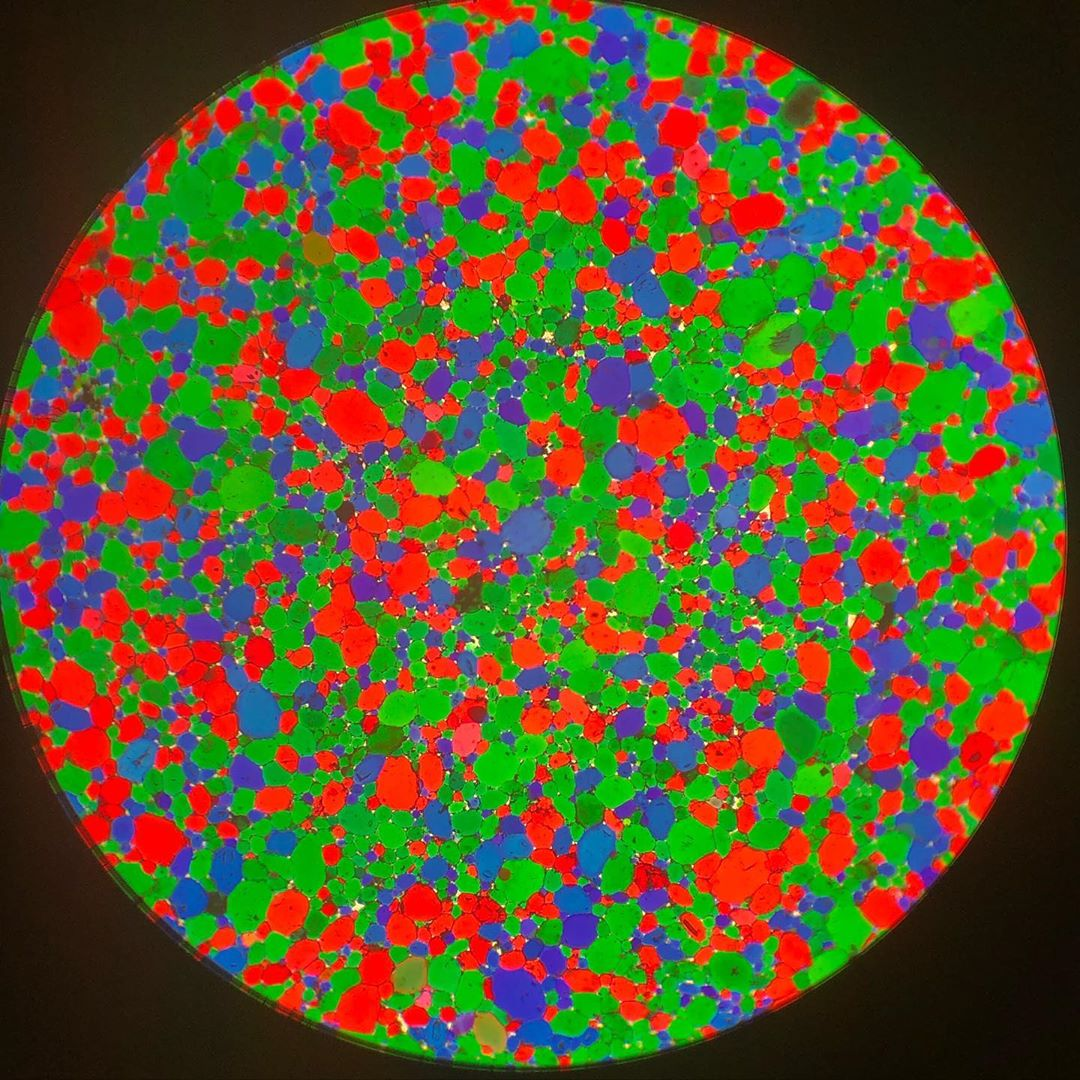
\includegraphics[width=4cm, height=4cm]{img/part1_23.jpg}
\end{center}

The compression step can be frustrating, time-intensive and somewhat difficult, but it's definitely far from impossible. While I use a modified CNC router to do most of the hard work these days, good results can be achieved by hand, and fairly inexpensively to boot. I'll discuss the ins and outs of each, starting with hand pressing.\newline

\textbf{Hand Pressing}\newline

I found out early on that relatively satisfactory results could be easily achieved just by smashing the starch with a spoon. However, this way proved to take a ridiculously long time to cover, say, a 4x5 plate. I tried a few things, including knitting needles and those 10mL rollerball bottles used for perfume and essential oils. My best results were achieved with the 1" transfer ball that I mentioned earlier in Part 4.\newline

I like to wipe the excess oil off the castor ball with a paper towel first before getting started. Gripping the castor ball in your hand, start rolling in on the plate in small little circles, slowly working your way across the whole plate. This whole step is very reminiscent of shading in a drawing with a pencil. In my experience, small circles help avoid the ball bearing seizing up. I've noticed that longer lines will often cause the ball to lock up, and usually ends up in the bearing scratching a large streak.\newline

You can expect this to take about 30-45 minutes for a 4x5 sized plate. It's a painfully slow process when you have a lot of plates to do -- I used to do a little bit of pressing whenever I was waiting on something to cook, or needed a break from work. Doing a bunch all at once is apt to make your fingers sore!\newline

%Link to vid2

The following plates were all made with hand-pressed starch:

\begin{center}
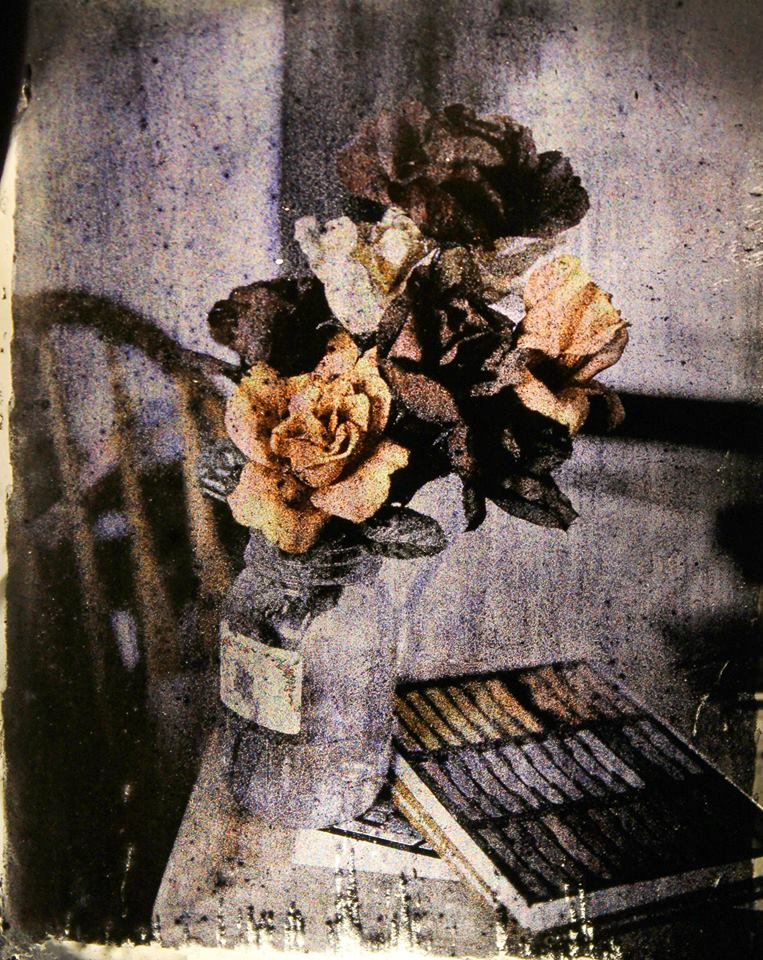
\includegraphics[width=4cm, height=4cm]{img/part1_24.jpg}
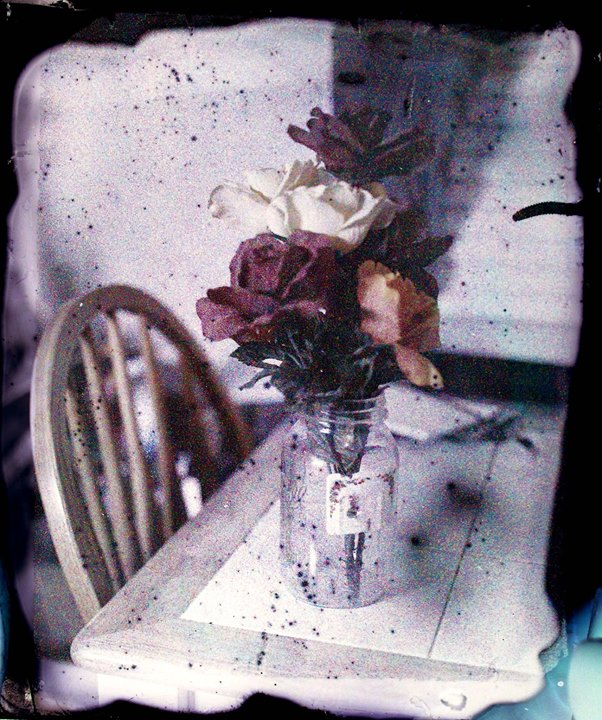
\includegraphics[width=4cm, height=4cm]{img/part1_25.jpg}
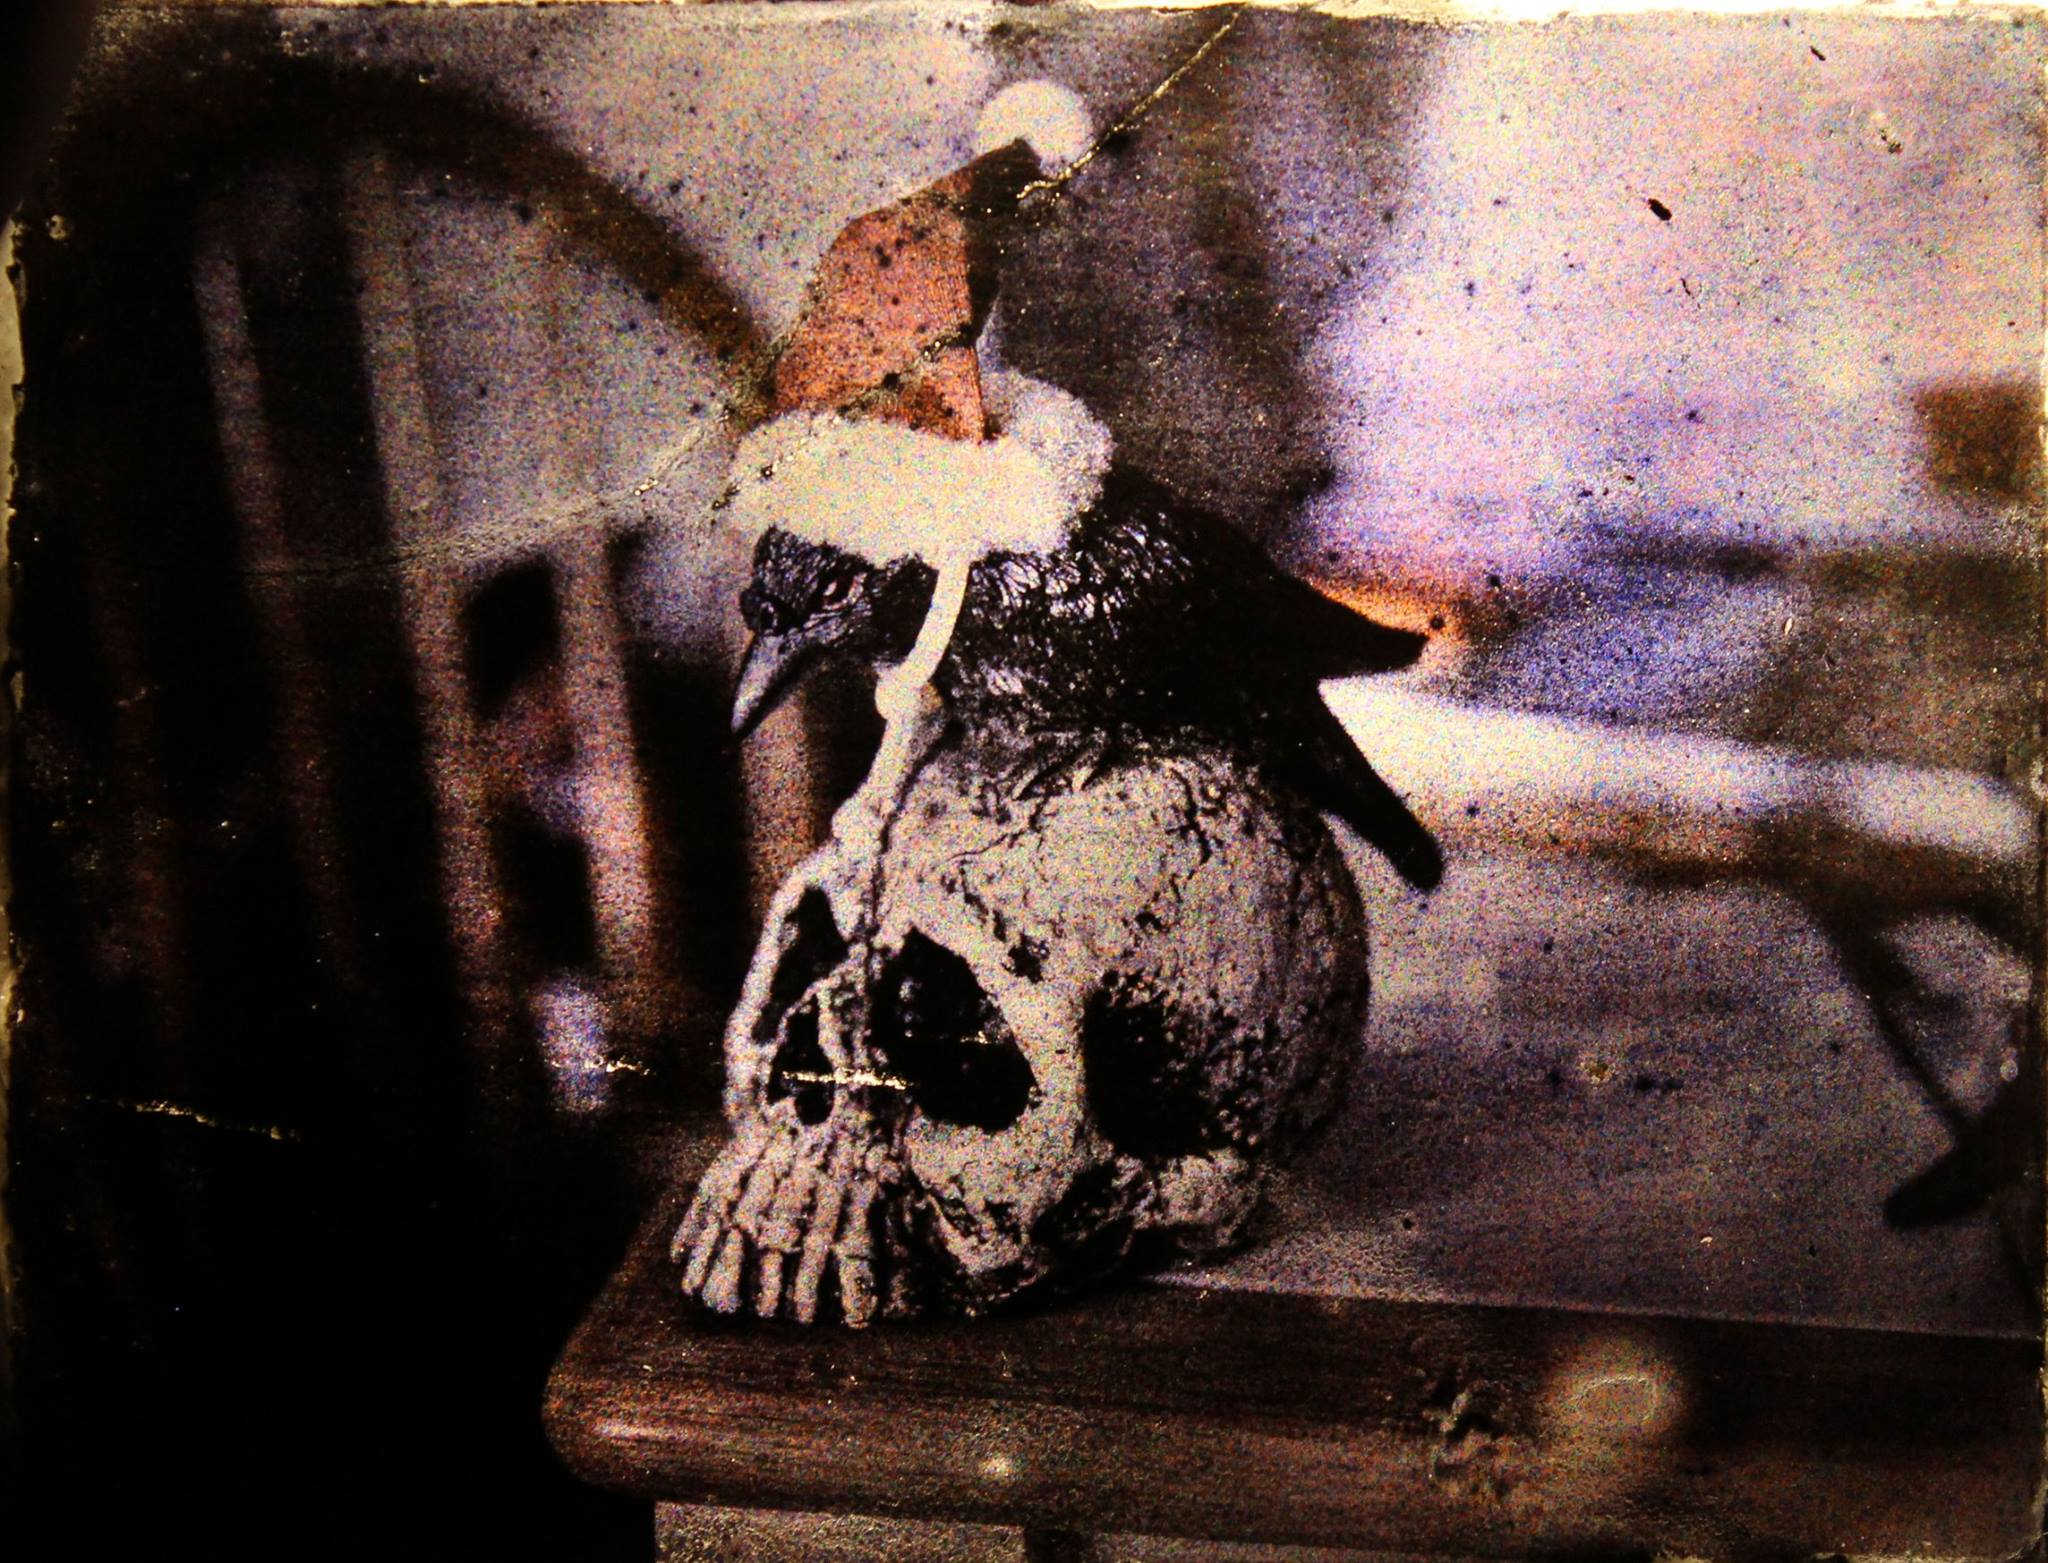
\includegraphics[width=4cm, height=4cm]{img/part1_26.jpg}
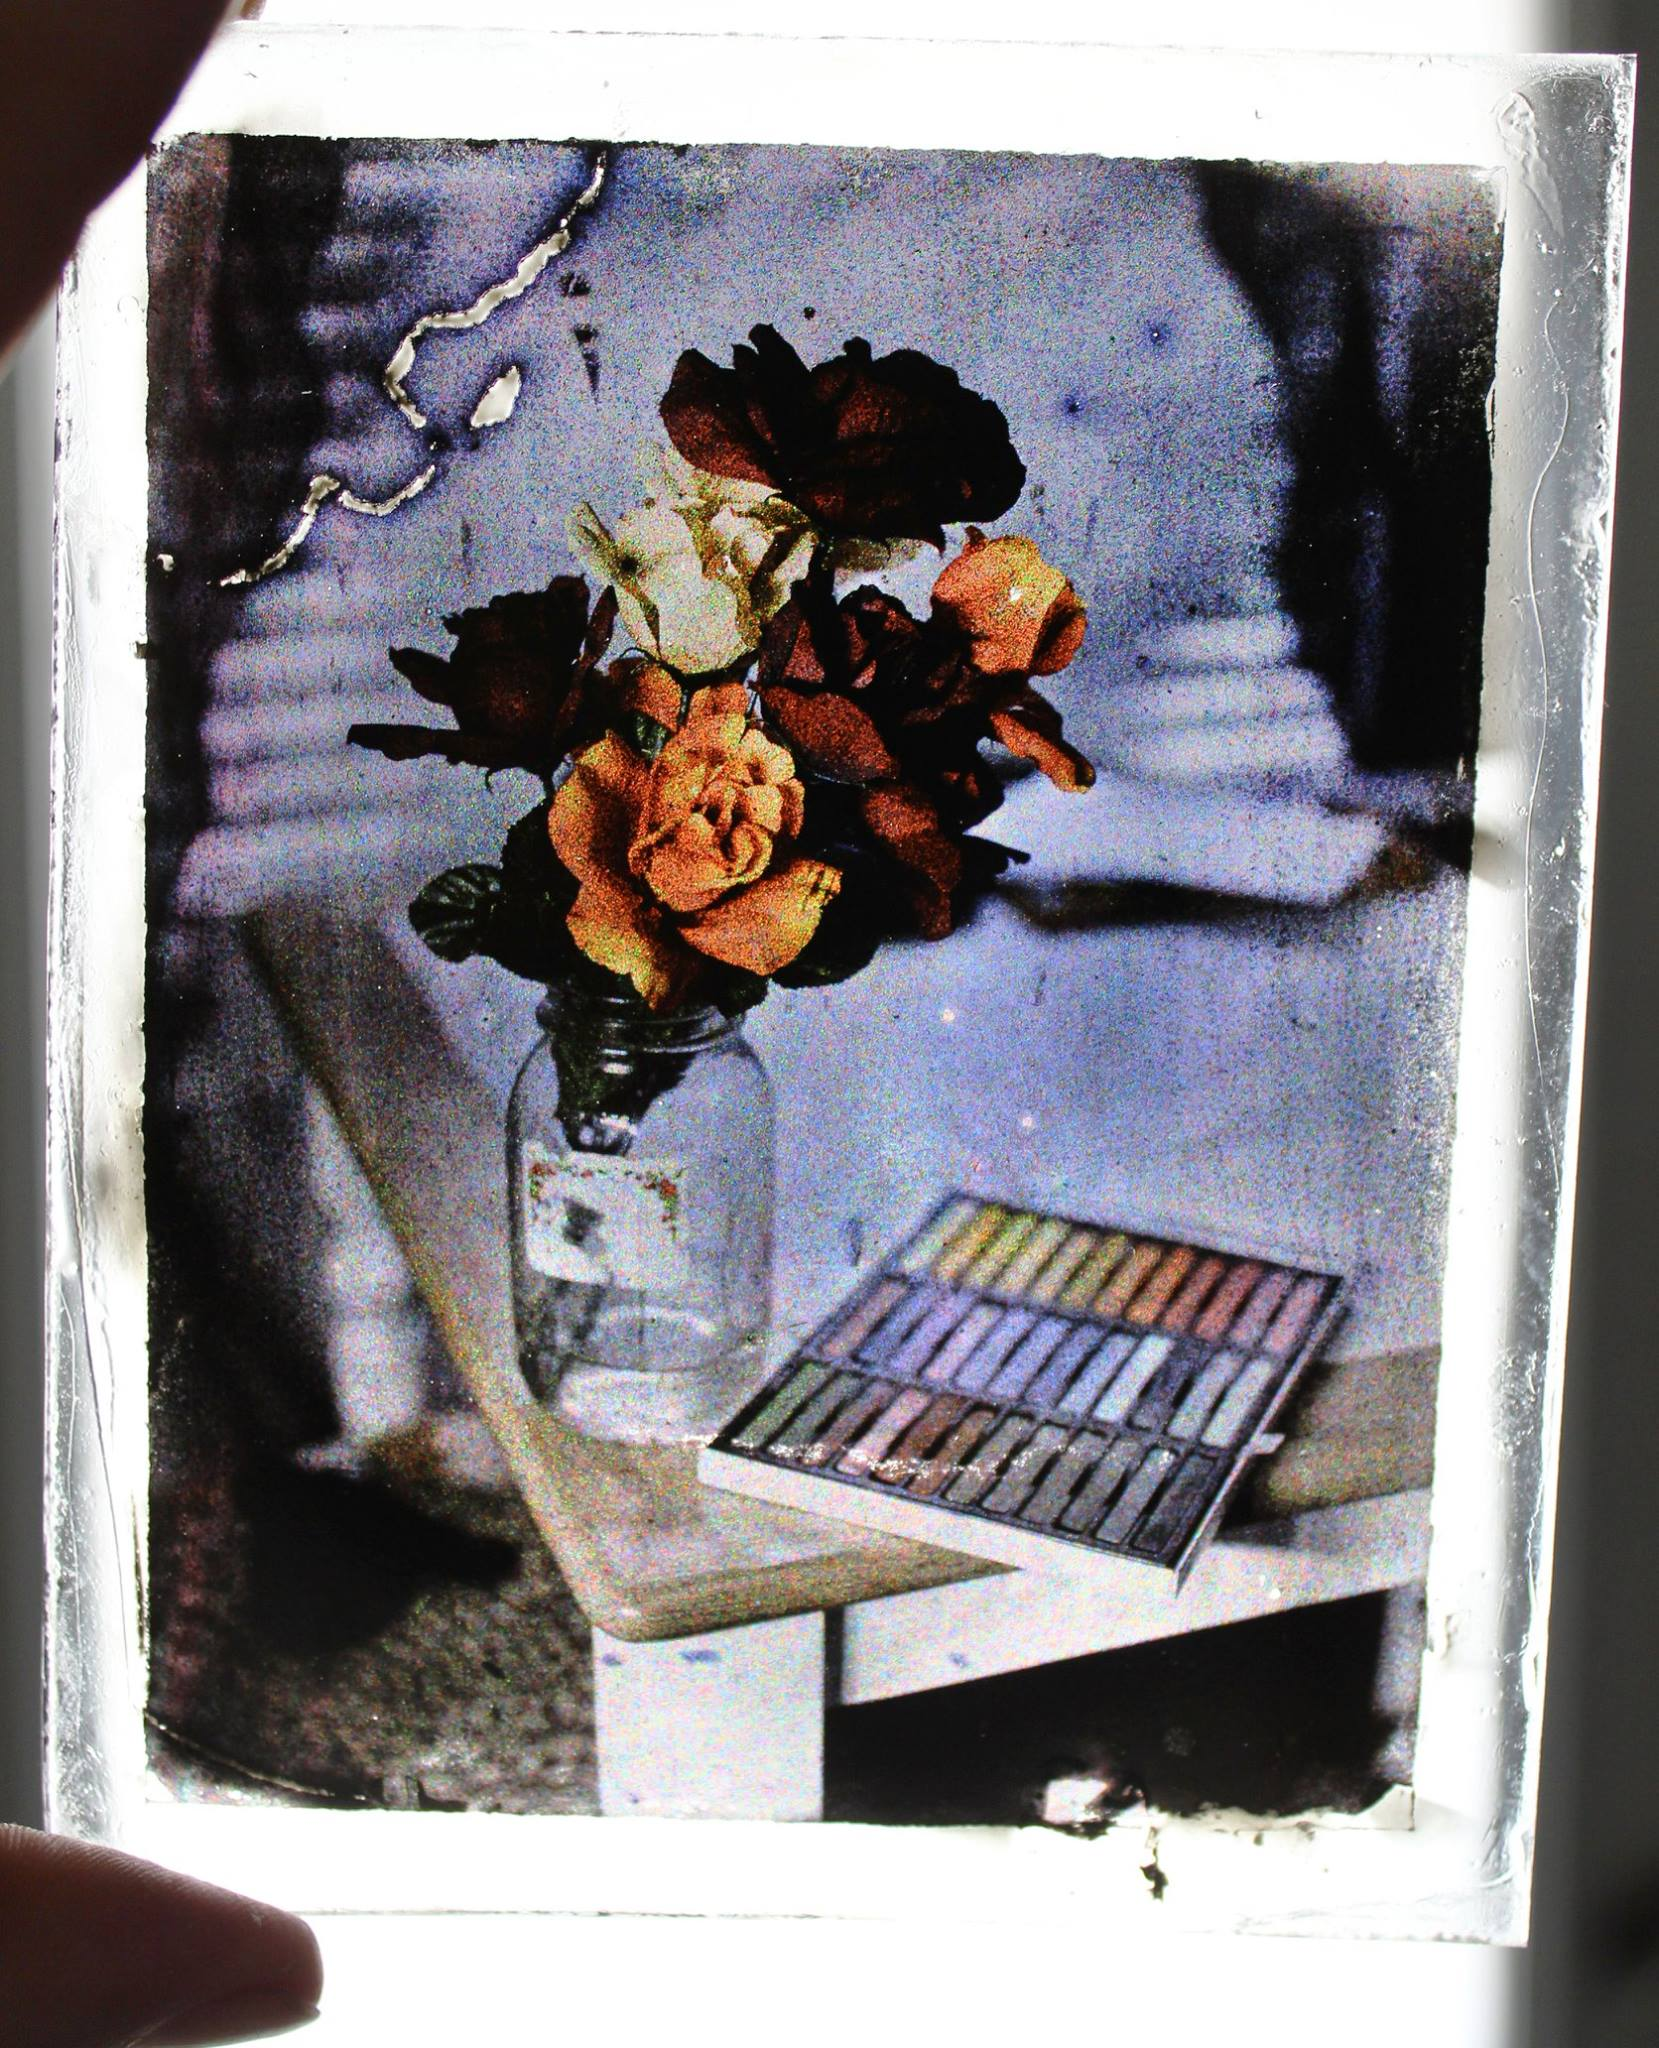
\includegraphics[width=4cm, height=4cm]{img/part1_27.jpg}
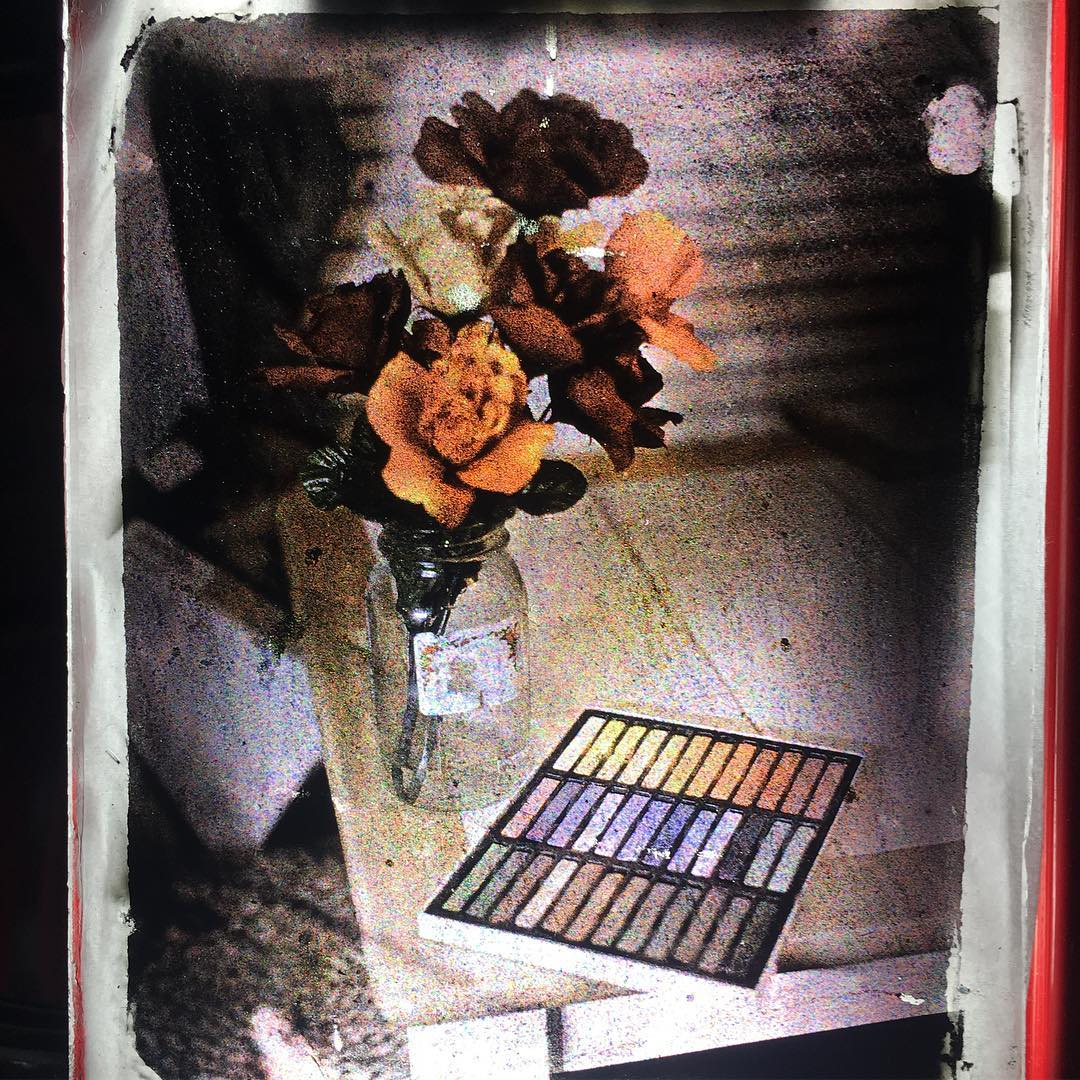
\includegraphics[width=4cm, height=4cm]{img/part1_28.jpg}
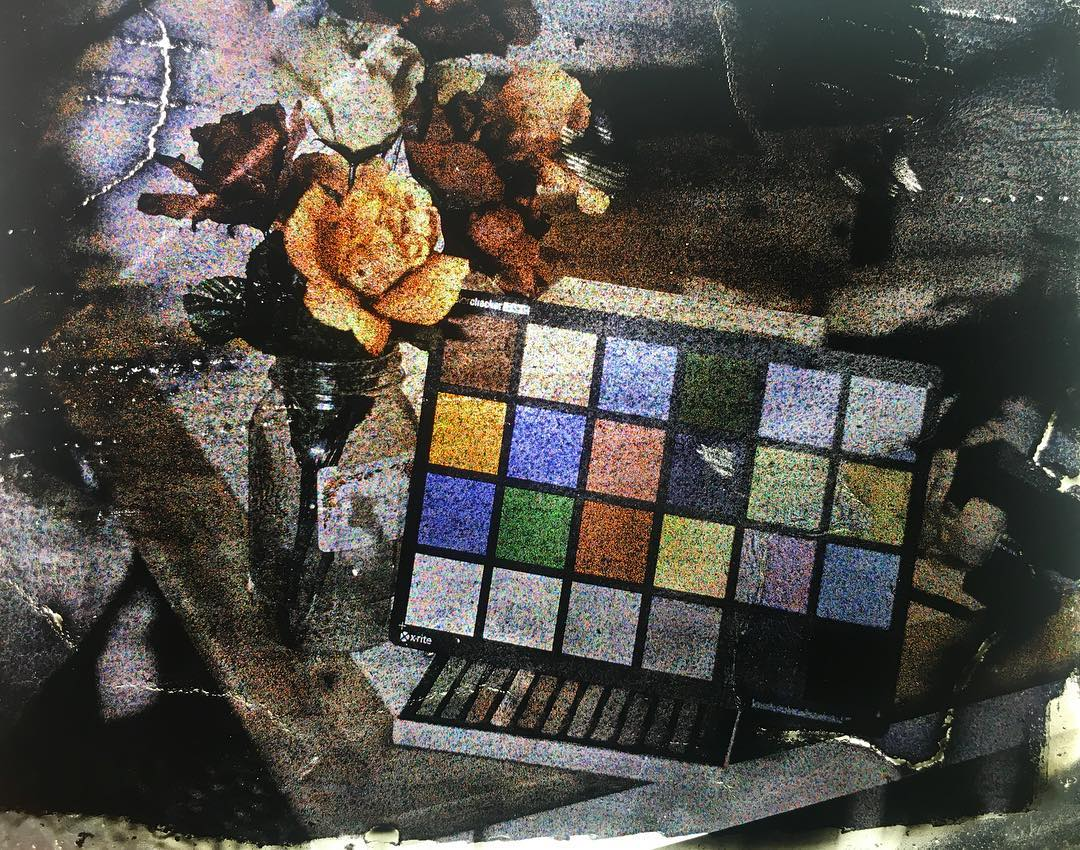
\includegraphics[width=4cm, height=4cm]{img/part1_29.jpg}
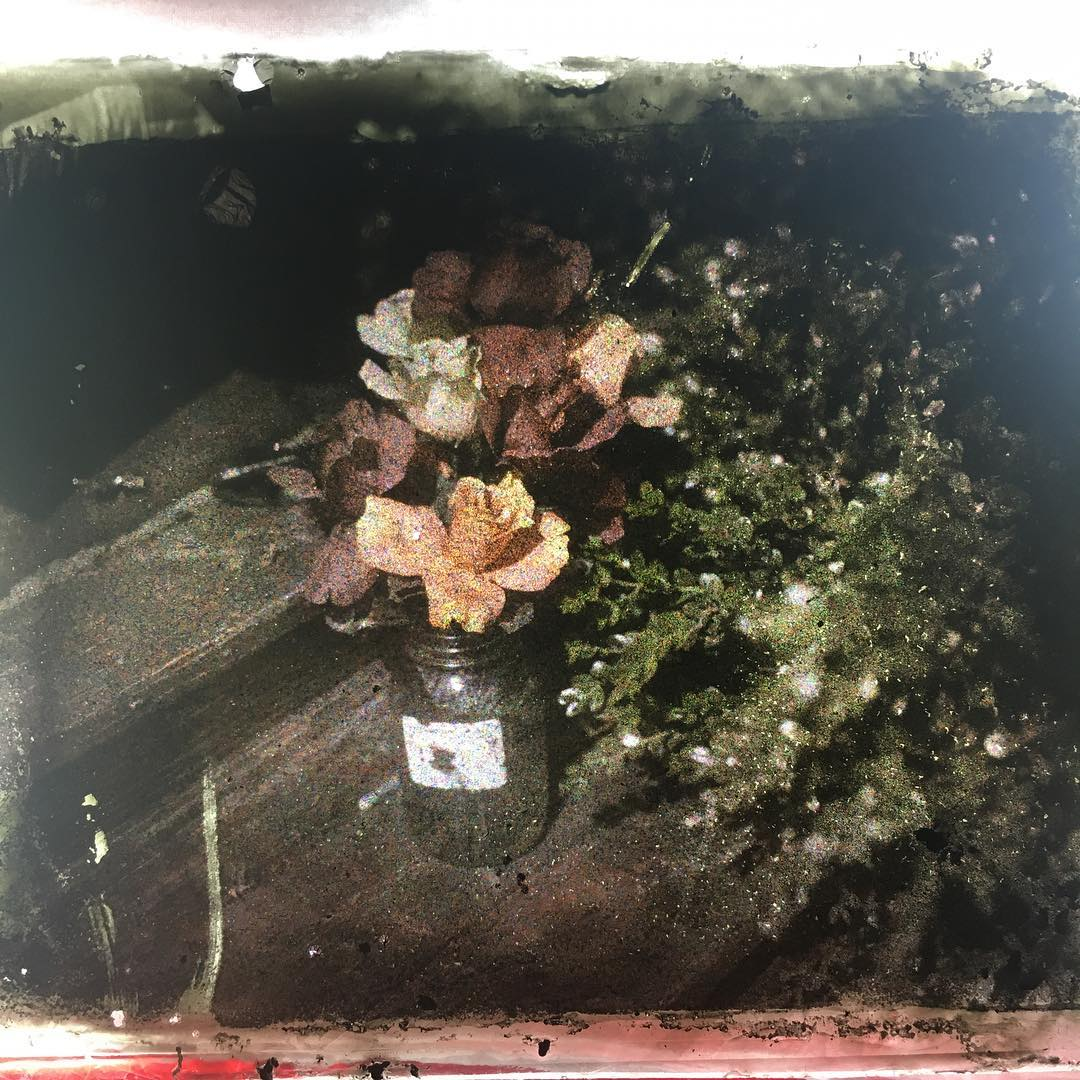
\includegraphics[width=4cm, height=4cm]{img/part1_30.jpg}
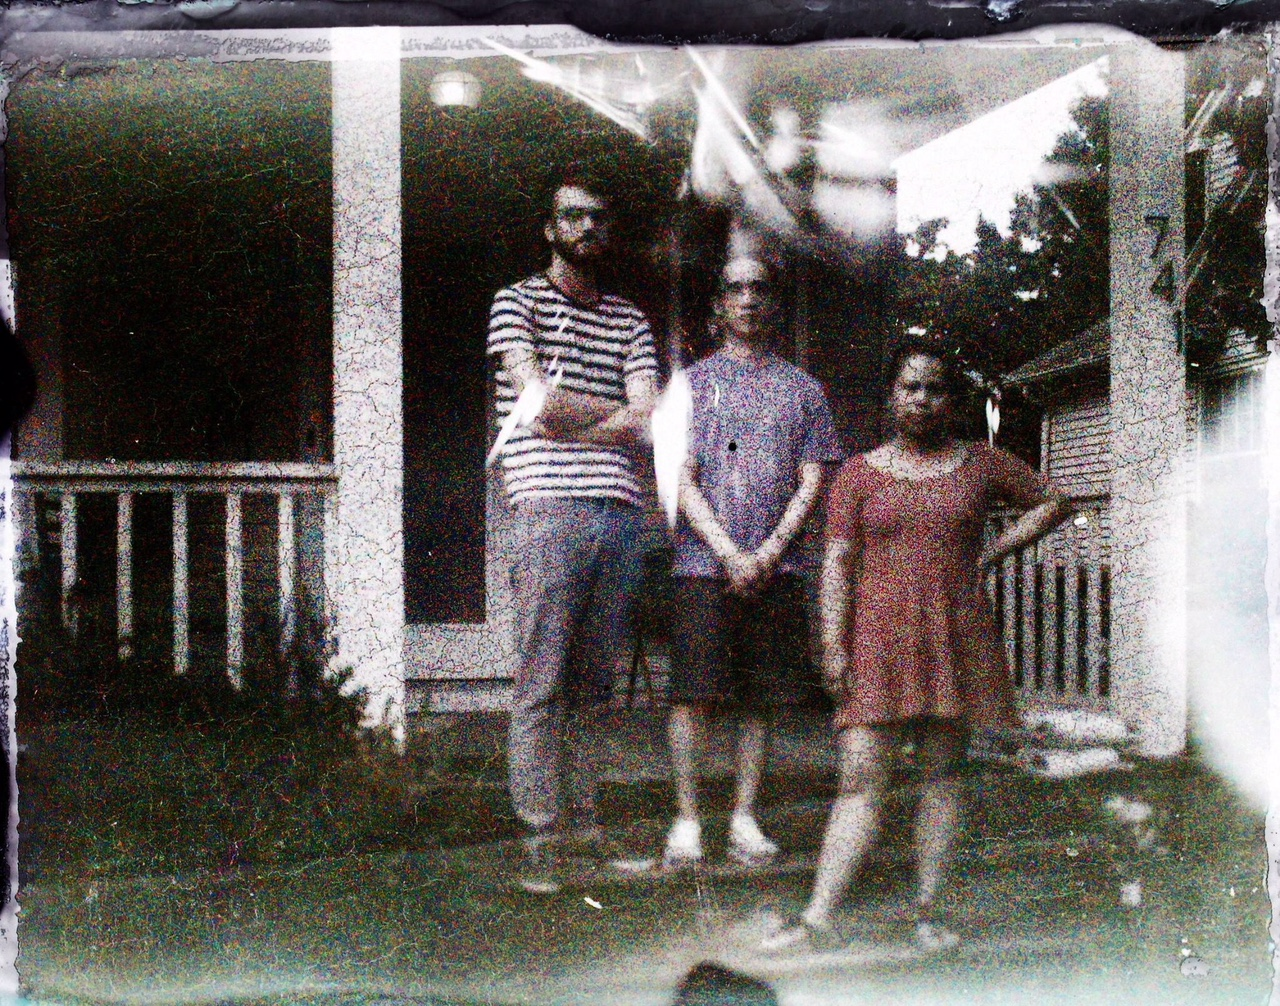
\includegraphics[width=4cm, height=4cm]{img/part1_31.jpg}
\end{center}

%You can expect this to take about 30-45 minutes for a 4x5 sized plate. It's a painfully slow process when you have a lot of plates to do -- I used to do a little bit of pressing whenever I was waiting on something to cook, or needed a break from work. Doing a bunch all at once is apt to make your fingers sore!\newline

\textbf{Machine Pressing}\newline

Pressing the starch by machine is infinitely less tedious and cleaner results can be obtained. With a roller and CNC setup like I've been using for the last year or so, a 4x5 plate can be pressed in about 10 - 15 minutes, and is much more of a "set and forget" type of process.\newline

Initially I used a Shapeoko 3 CNC router to press plates. The router is fully belt-driven, which means it's motion is very quick compared to an axis with ballscrew. I'm not sure if this was a problem limited to my particular model, or if all Shapeokos suffer from this, but unfortunately the z-axis belt would skip if too much downward force was applied. This limited roller to 1) have an extremely small contact area and 2) require multiple passes to achieve a satisfactory pressing. In general I found that the plate would require about 14 passes to achieve a satisfactory degree of compression. With this style of roller, it took about 45 minutes to press a 4x5 plate.\newline

The roller was made from a window guide-roller, with a 1/4" bolt as an axis. The sides of the roller were sanded down to be a little less sharp, as it tended to cut into the plate and leave big lines.\newline

%Link to vid3

Next, I tried a lower-end 3040 CNC machine that uses all ballscrew axes. The overall travel motion is slower, but the ballscrew z-axis allows the machine to apply more downward force on the plate. I've iterated through a few different roller designs, but have had the best consistent success with a polycarbonate one designed for a Creality Cr-10. The frame is made from laser cut 1/4" plywood, and uses an M5 bolt as an axis.\newline

\begin{center}
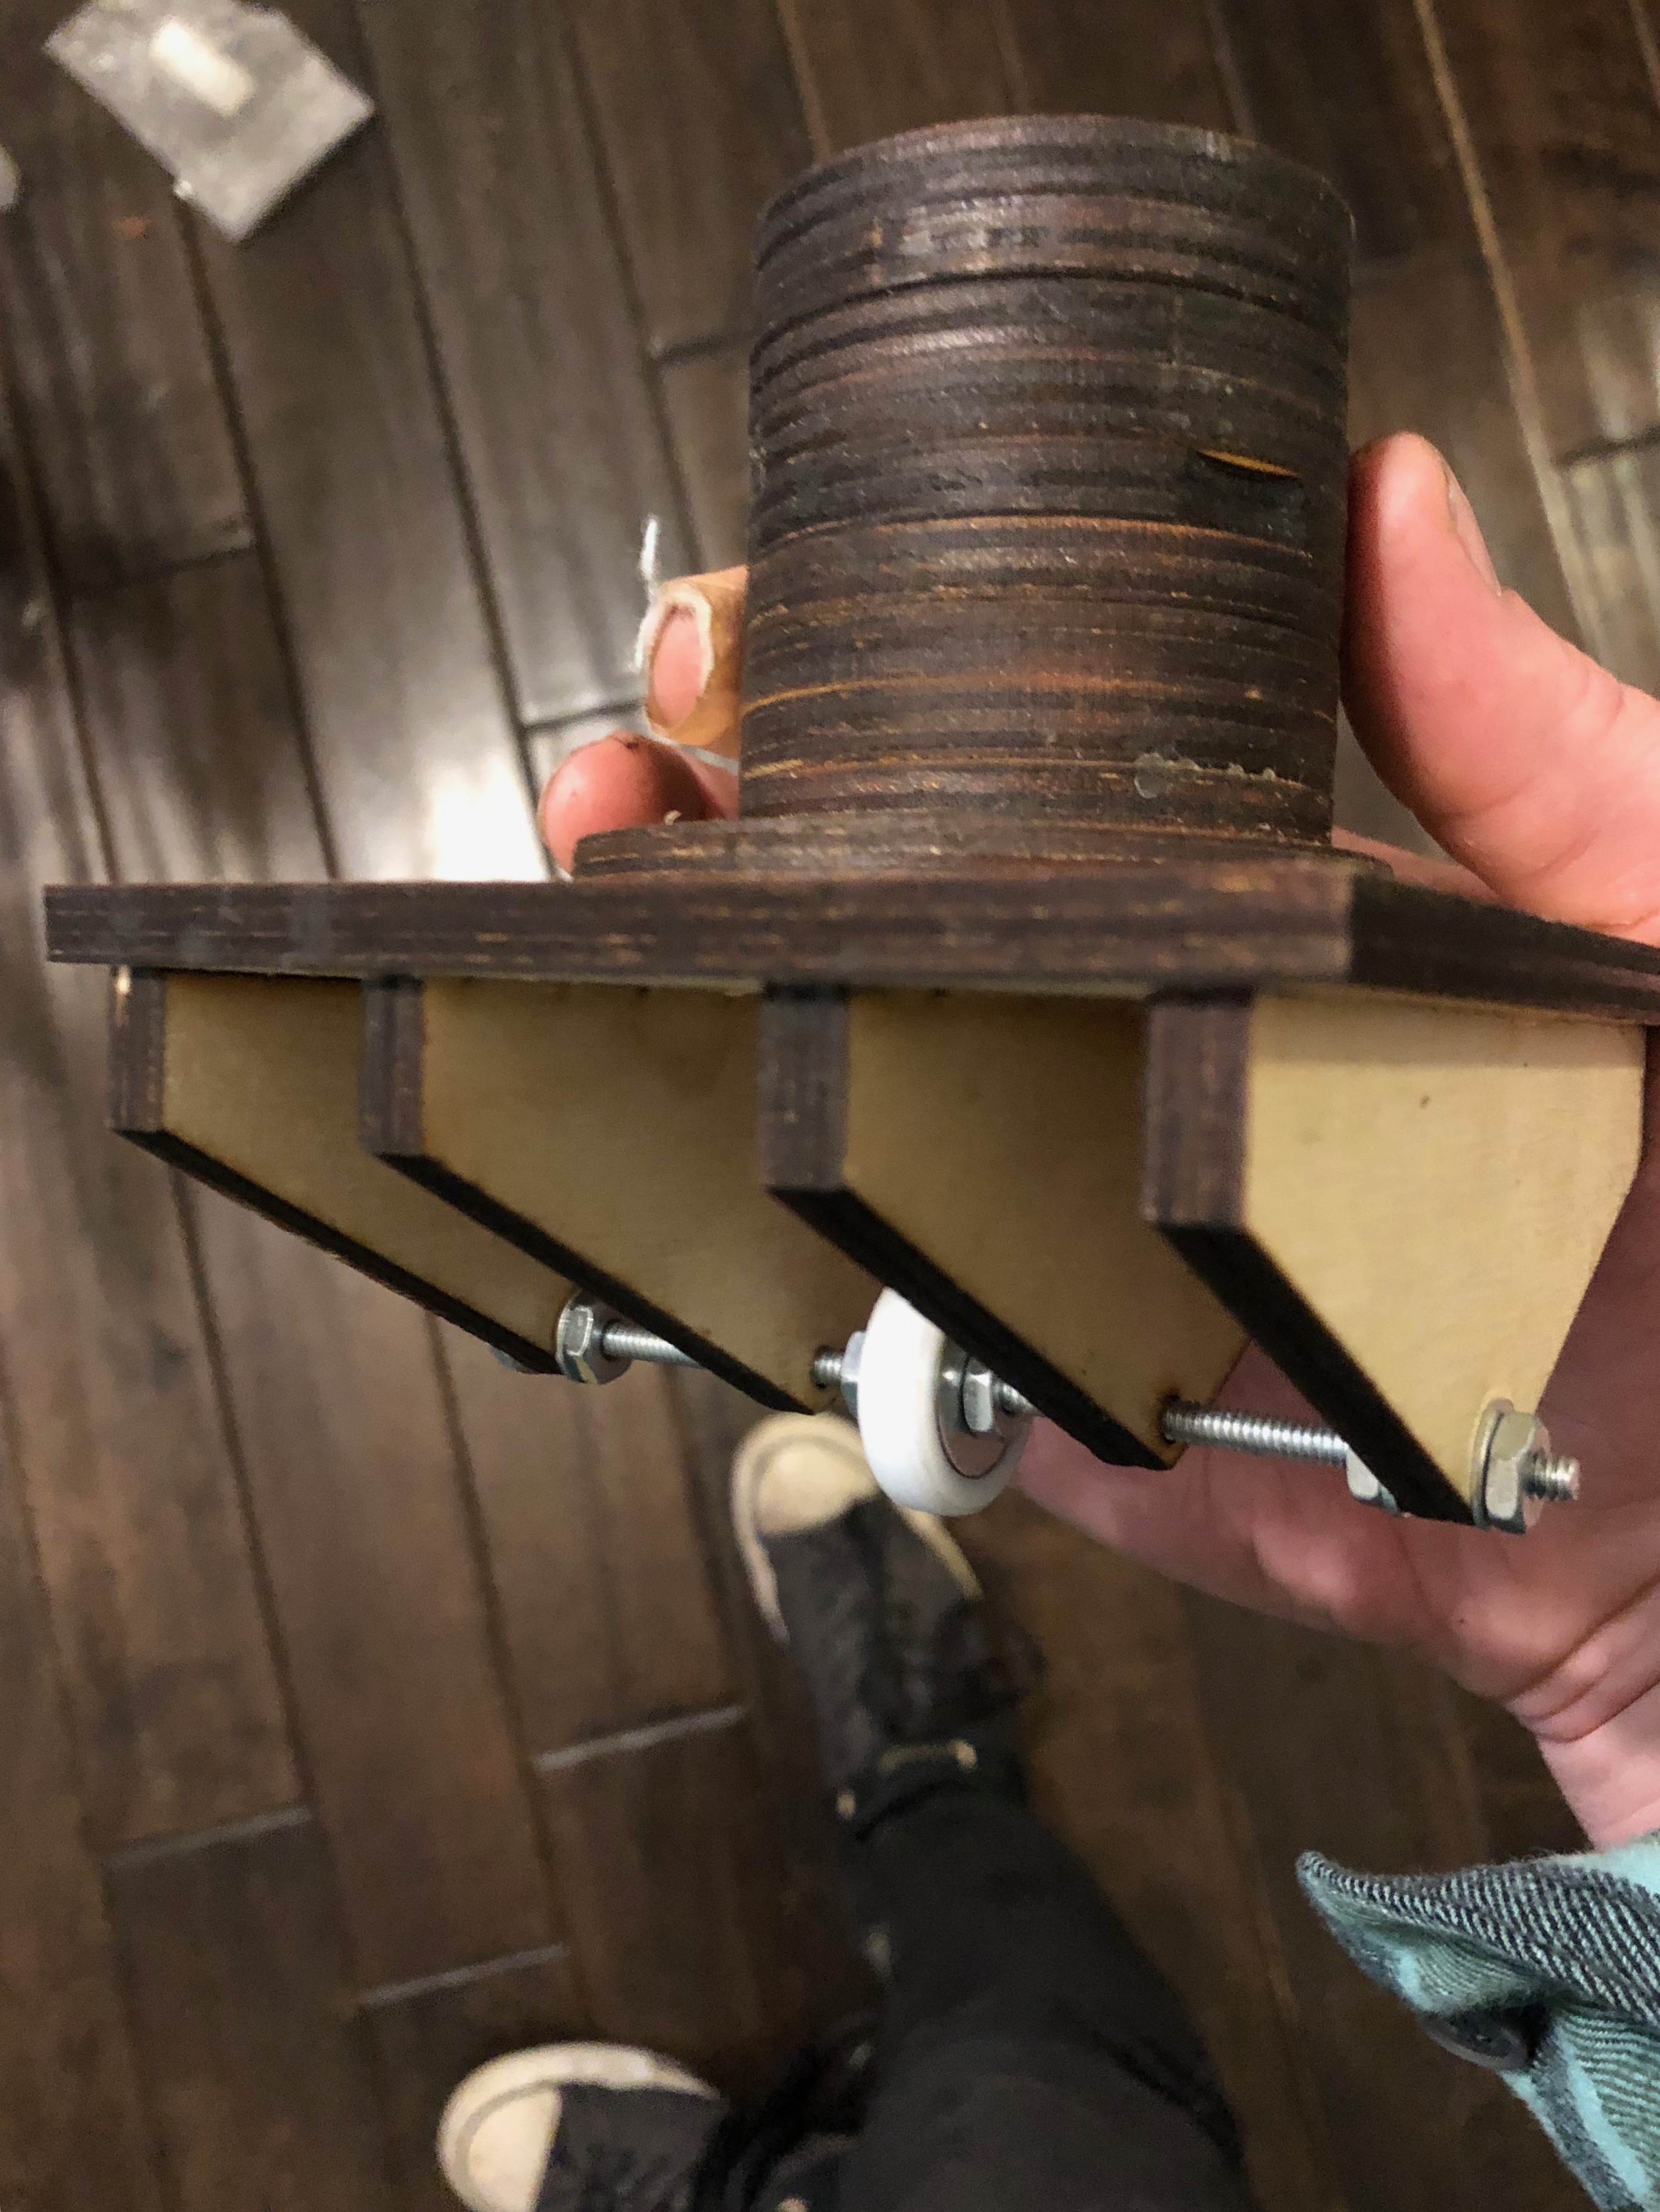
\includegraphics[width=5cm, height=5cm]{img/part1_32.jpg}
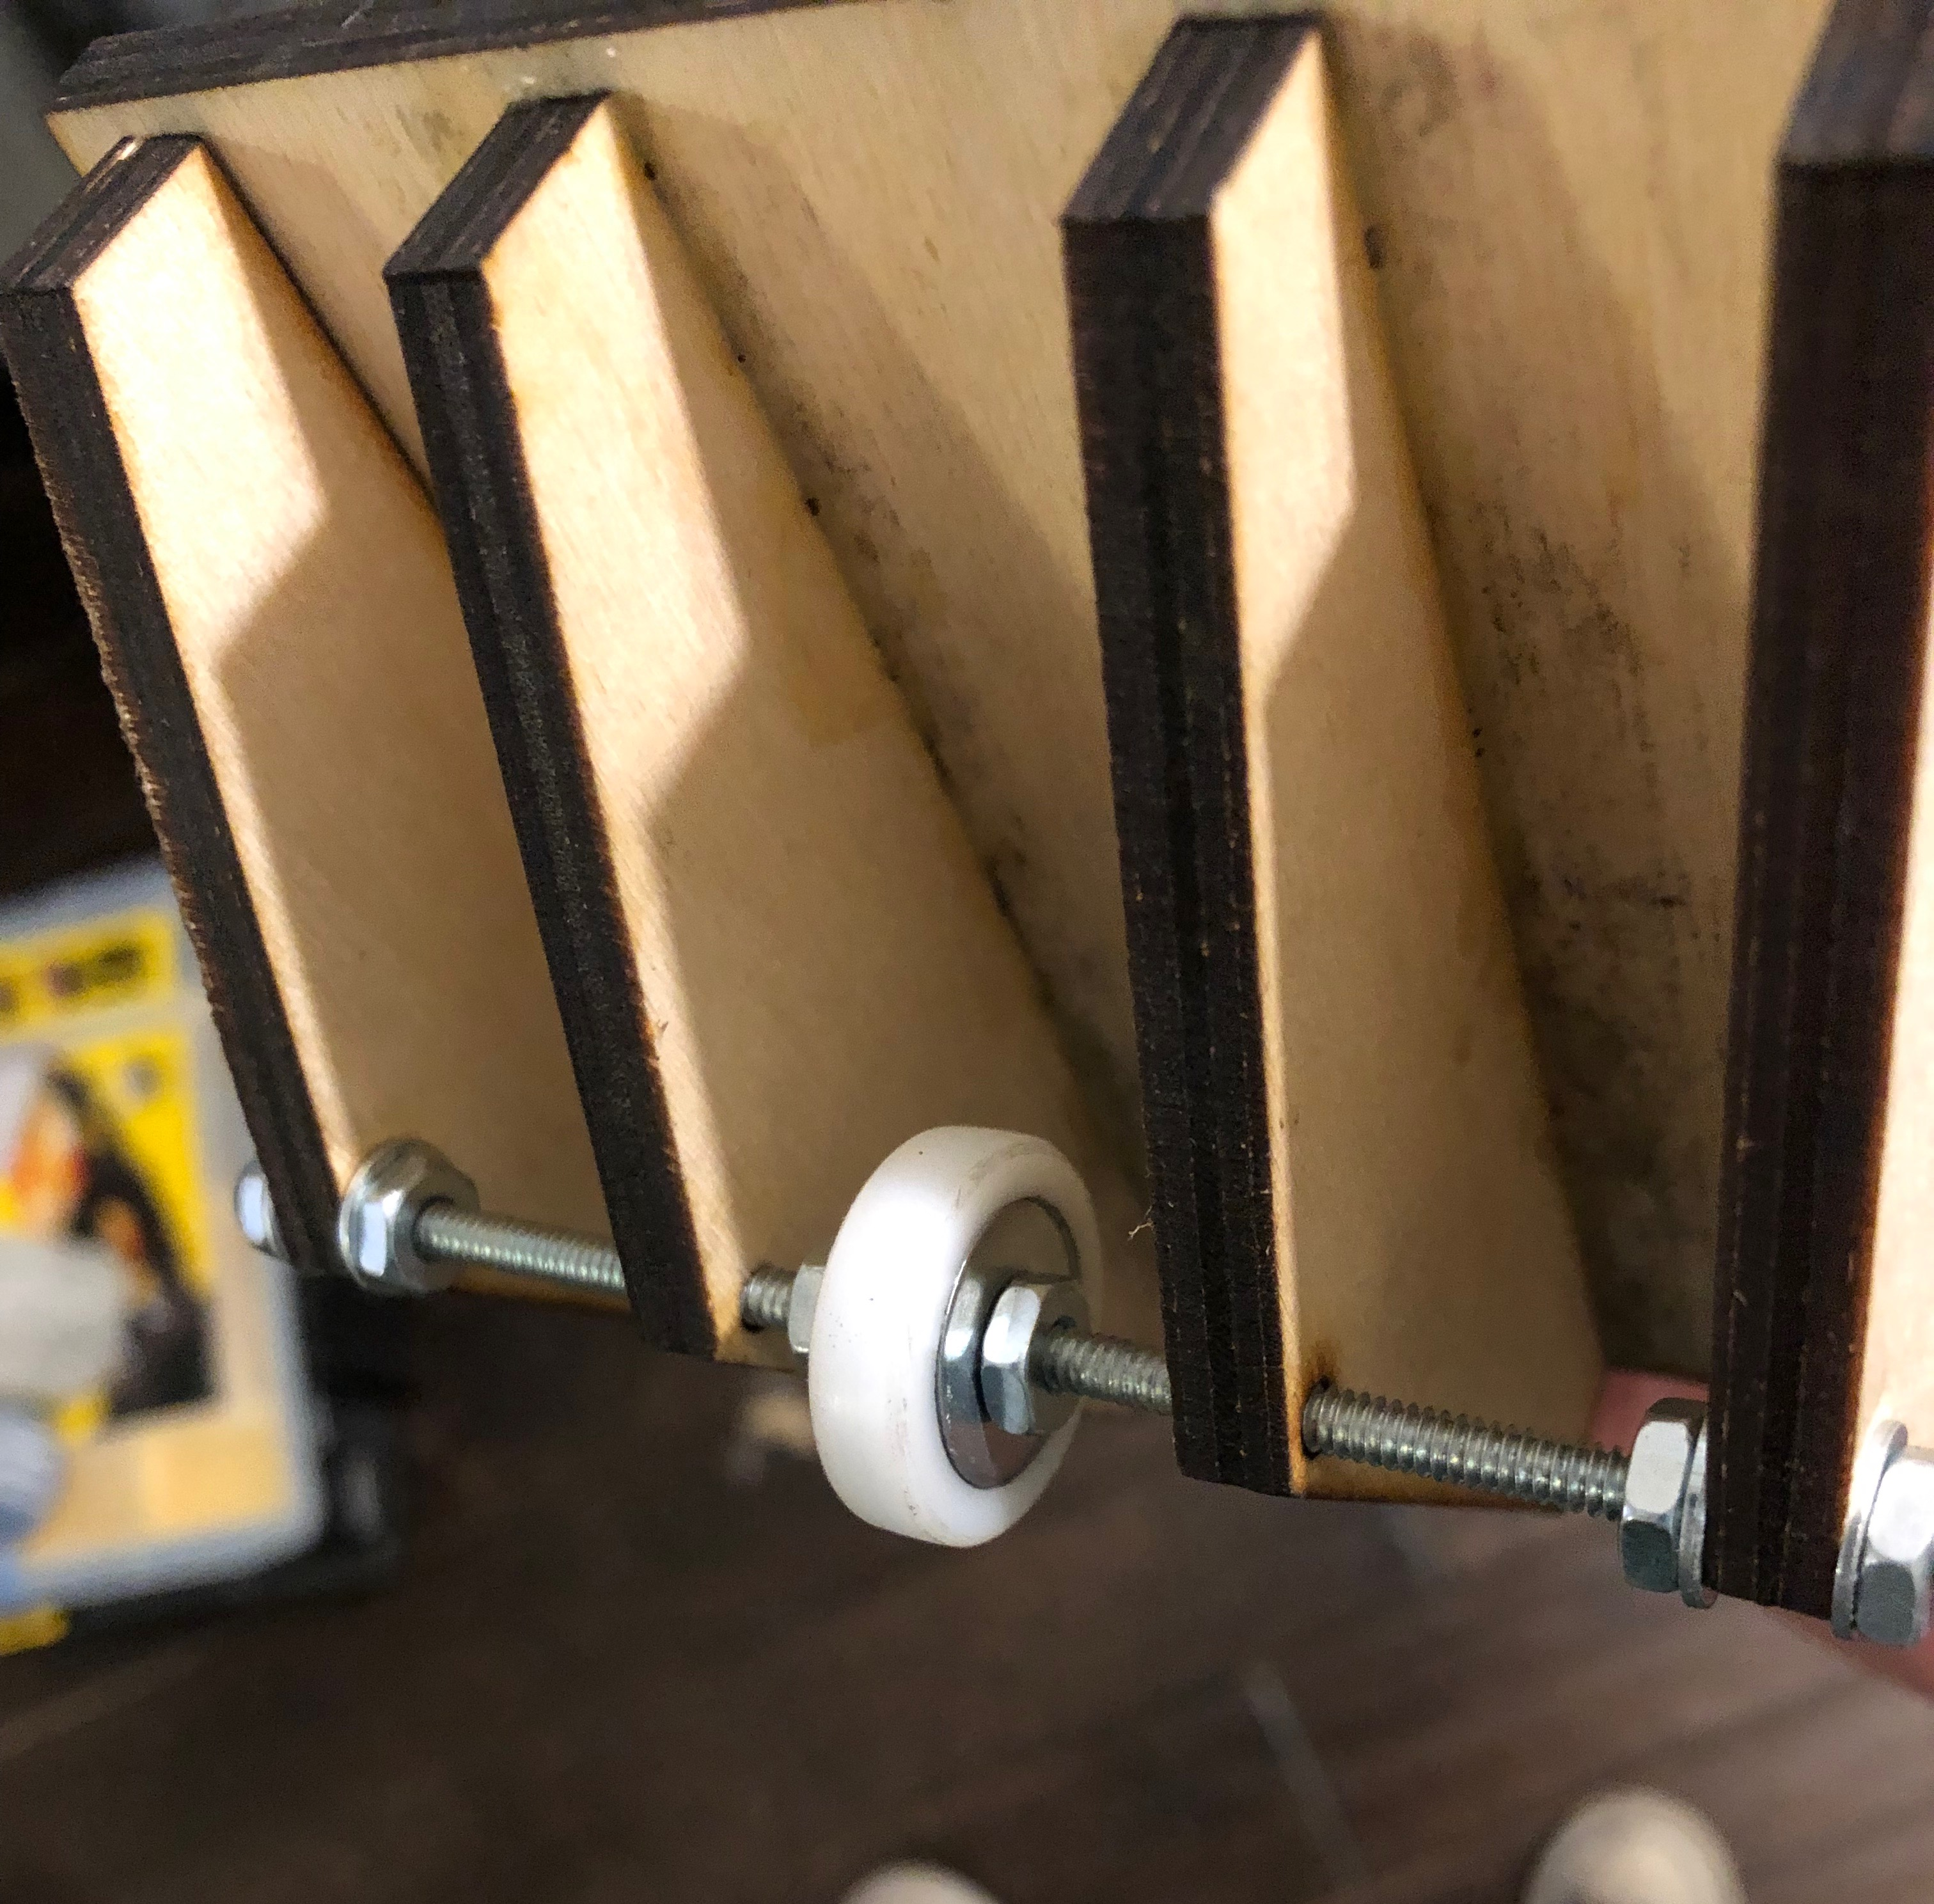
\includegraphics[width=5cm, height=5cm]{img/part1_33.jpg}
\end{center}

To avoid sharper edges of the wheel cutting into the plate, the whole wheel will need to be sanded carefully.\newline

As mentioned, despite the fact that the machine travel speed is overall slower than the Shapeoko 3, the machine can apply more force to the plate, allowing the use of a wider roller and a single-pass motion across the plate. Typically a 4x5 plate can be fully pressed in about 15 minutes. Care must be taken, since this machine is able to apply enough force to crack the glass! An unattended machine will quickly pulverize the glass, damaging the roller.\newline

%Link to vid4

I home the x and y axes by jogging them up/left until no more motion is permitted and the stepper motor skips steps. Similarly, I home my z axis by jogging down into the plate until the motor skips. The axis cannot crack the glass without rolling back and fourth across the plate, so no worries here yet. The overall pressure applied by the roller can be varied by changing the z height in the program. For my machine, z=0.8mm is about as much pressure as a 4x5 plate can take before cracking becomes common.\newline

The base the plate rests on must be fairly rigid, as any amount of flex will crack the glass. MDF worked well for a while for 4x5 sized plates, but 5x7 sized plates would routinely bend too much and break apart. I changed the substrate to a thick piece of glass (1/4") which was decidedly less flexible, with improved results.\newline

If anyone wanted to try out machine pressing, I'd definitely recommend going with the 3040 version, rather than the Shapeoko. It's much cheaper (~600USD usually) and can reliably press plates much more quickly.\newline

After completing the pressing, I always laser engrave the edges of each plate. Numbering them has helped me a ton while experimenting with different second varnish coatings.\newline

%Link to vid5

\subsection{Making the Second Varnish}

I've tried a ton of different modern replacements for the second varnish, but I've found that nothing works quite as well as the good ol' original Lumiere recipe. Unfortunately, making it is a somewhat lengthy process, and will probably take a few days before it's ready.\newline

You'll be working with ethyl acetate a lot here. The fumes aren't particularly dangerous, but it is flammable and quite volatile, so make sure you're working with adequate ventilation.\newline

Start by taking 28.8g of damar gum, and grinding it up into chunks with a mortar and pestle. In a 500mL beaker, add about 250mL of ethyl acetate and a magnetic stirbar that you don't mind getting coated in a bunch of varnish. I tape some plastic wrap to the top, to cut down on the evaporation of the ethyl acetate. Stir for 5 or so minutes, and then let it sit for several hours. You'll notice a lot of the yellow alpha-resene starts to dissolve away, leaving behind the fine white waxy beta-resene. I repeat this for 2-3 days, until I've ensured all the alpha-resene has dissolved. I let it stand for a while until it's mostly clear.

\begin{center}
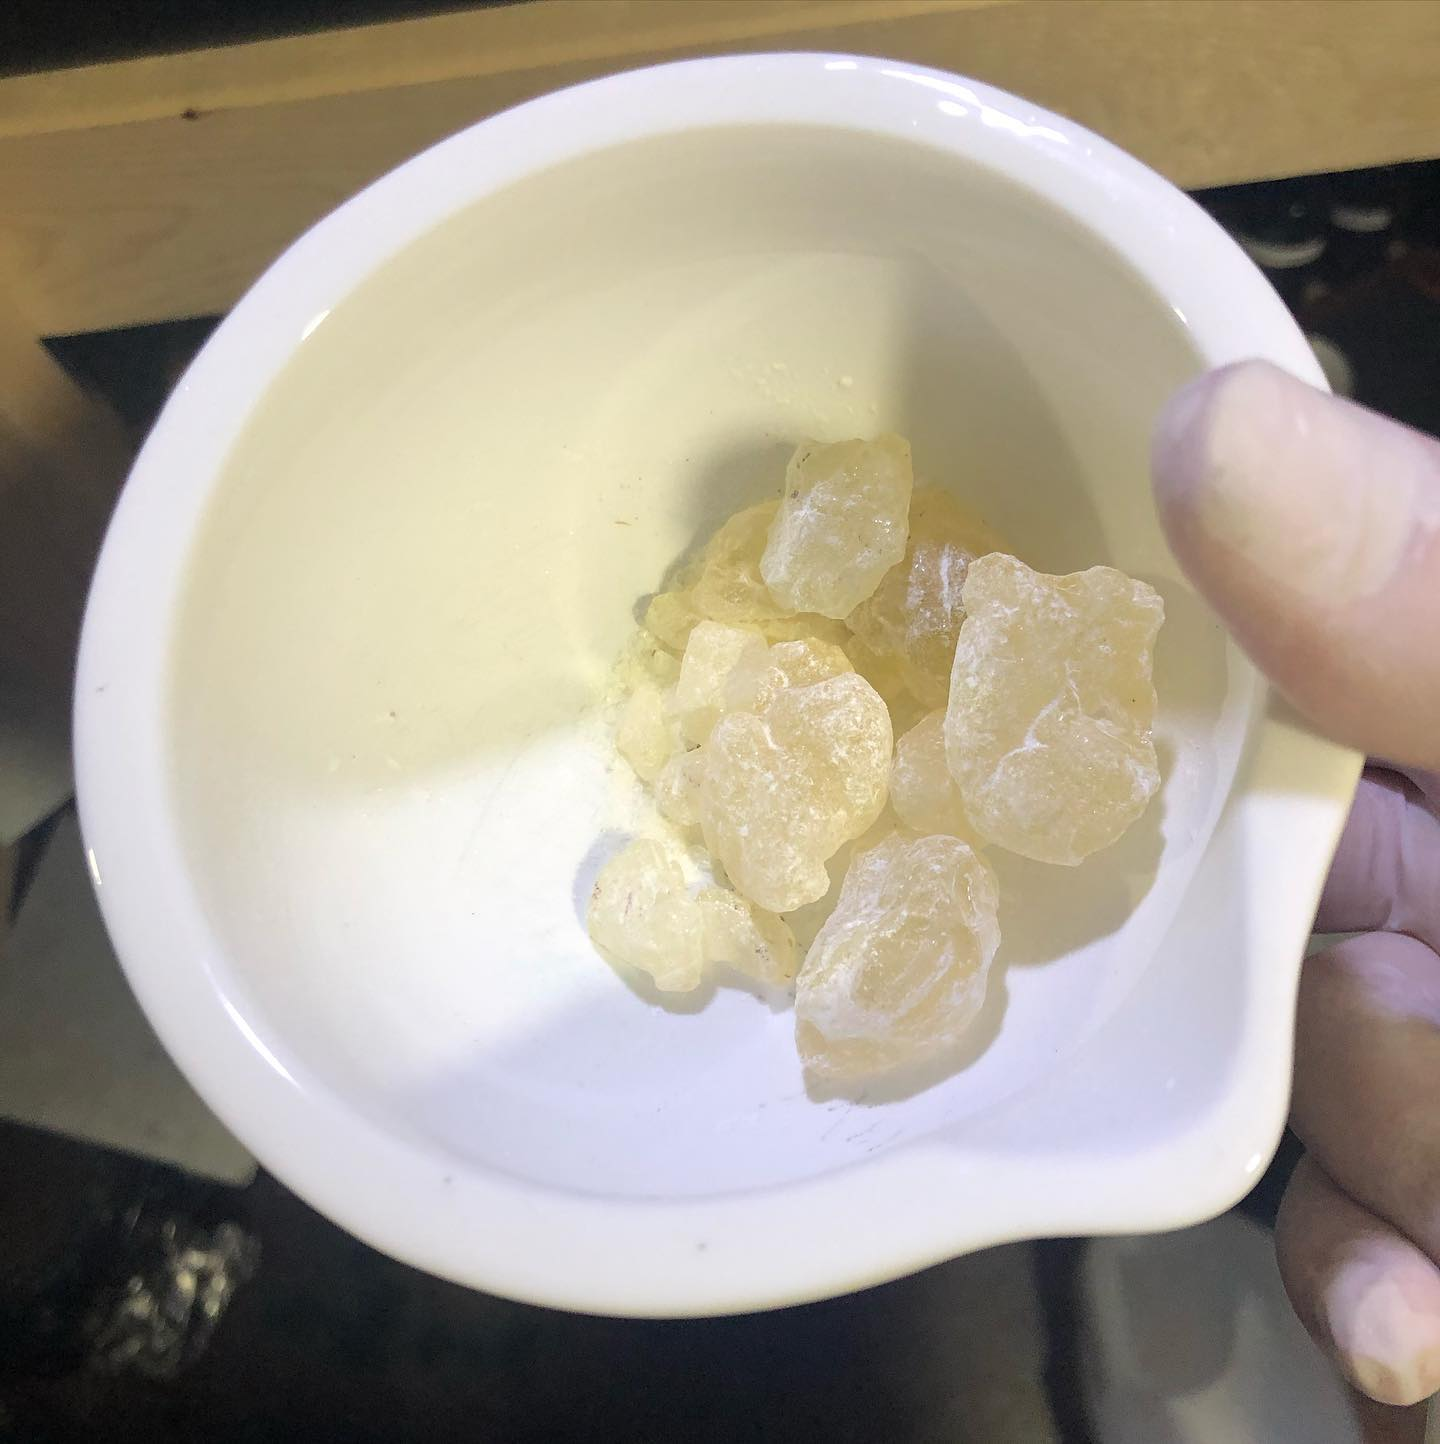
\includegraphics[width=4cm, height=4cm]{img/part1_34.jpg}
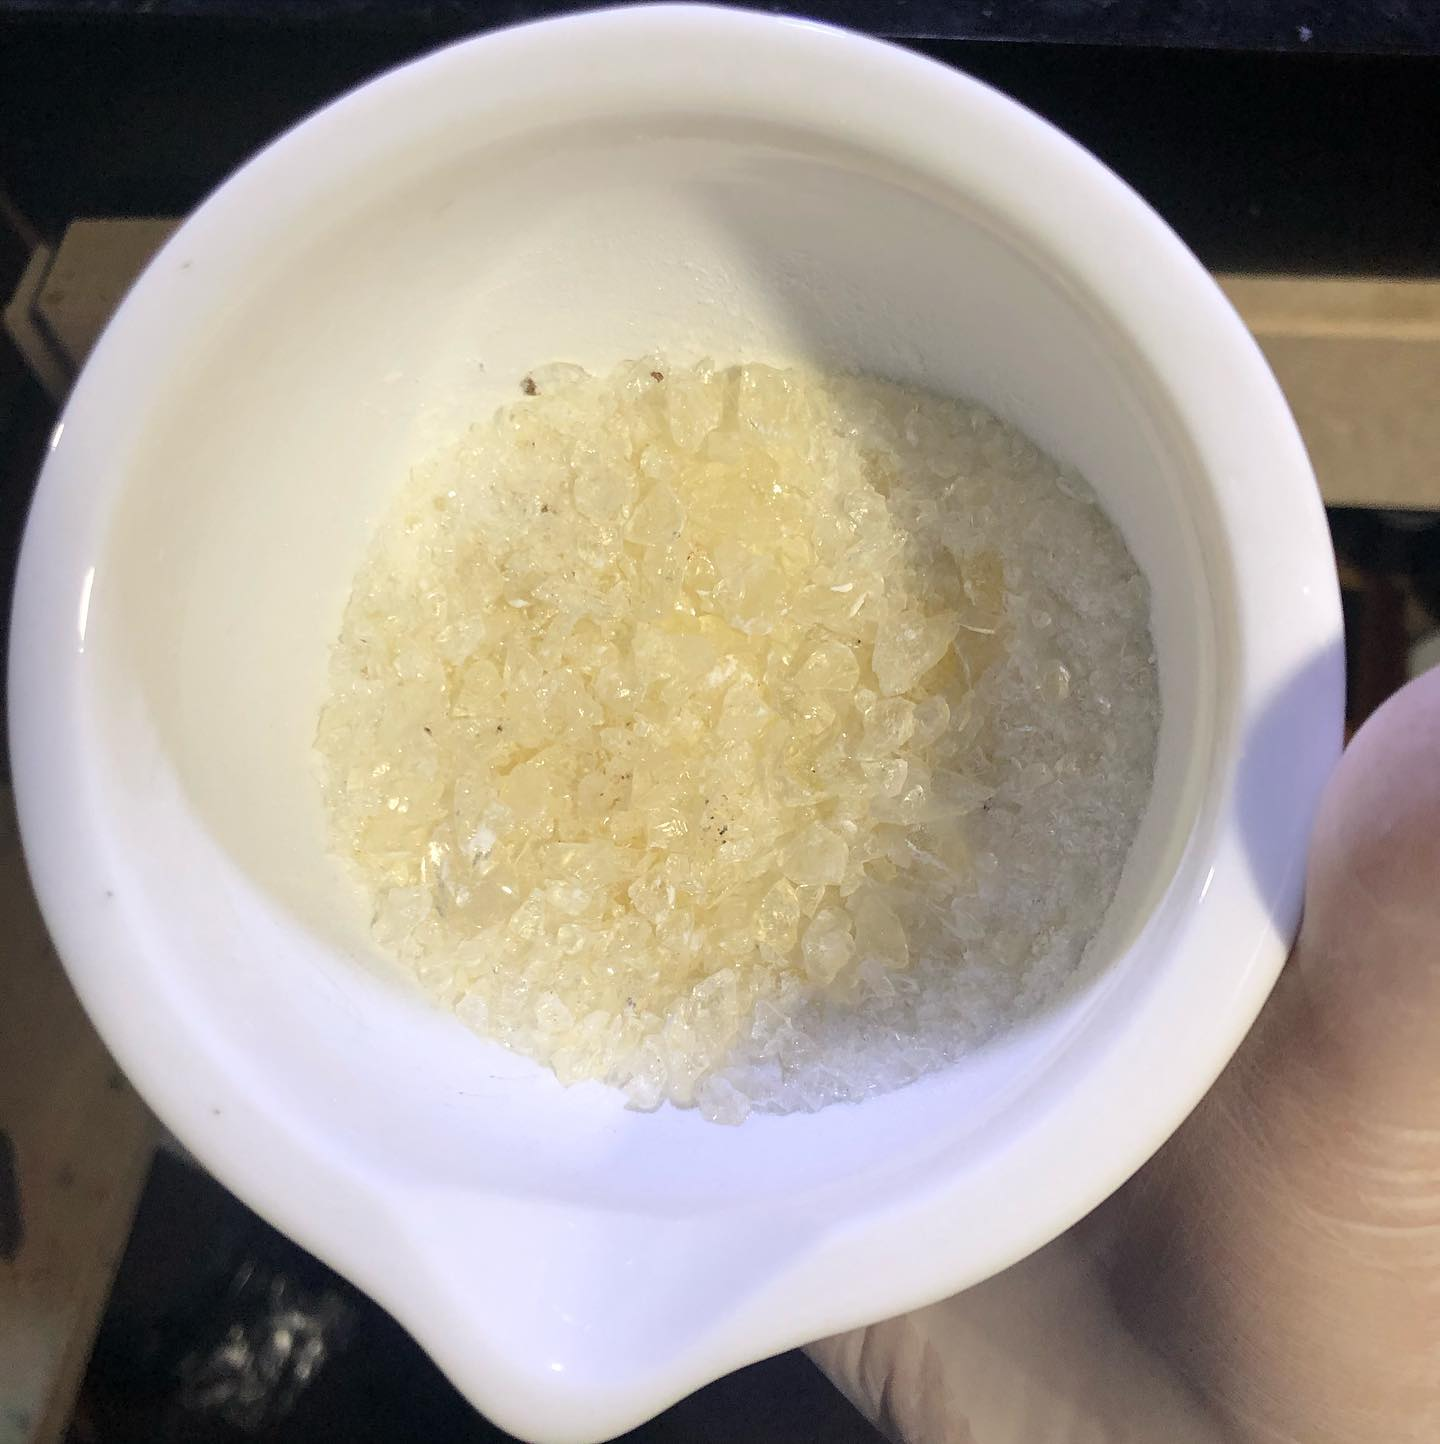
\includegraphics[width=4cm, height=4cm]{img/part1_35.jpg}
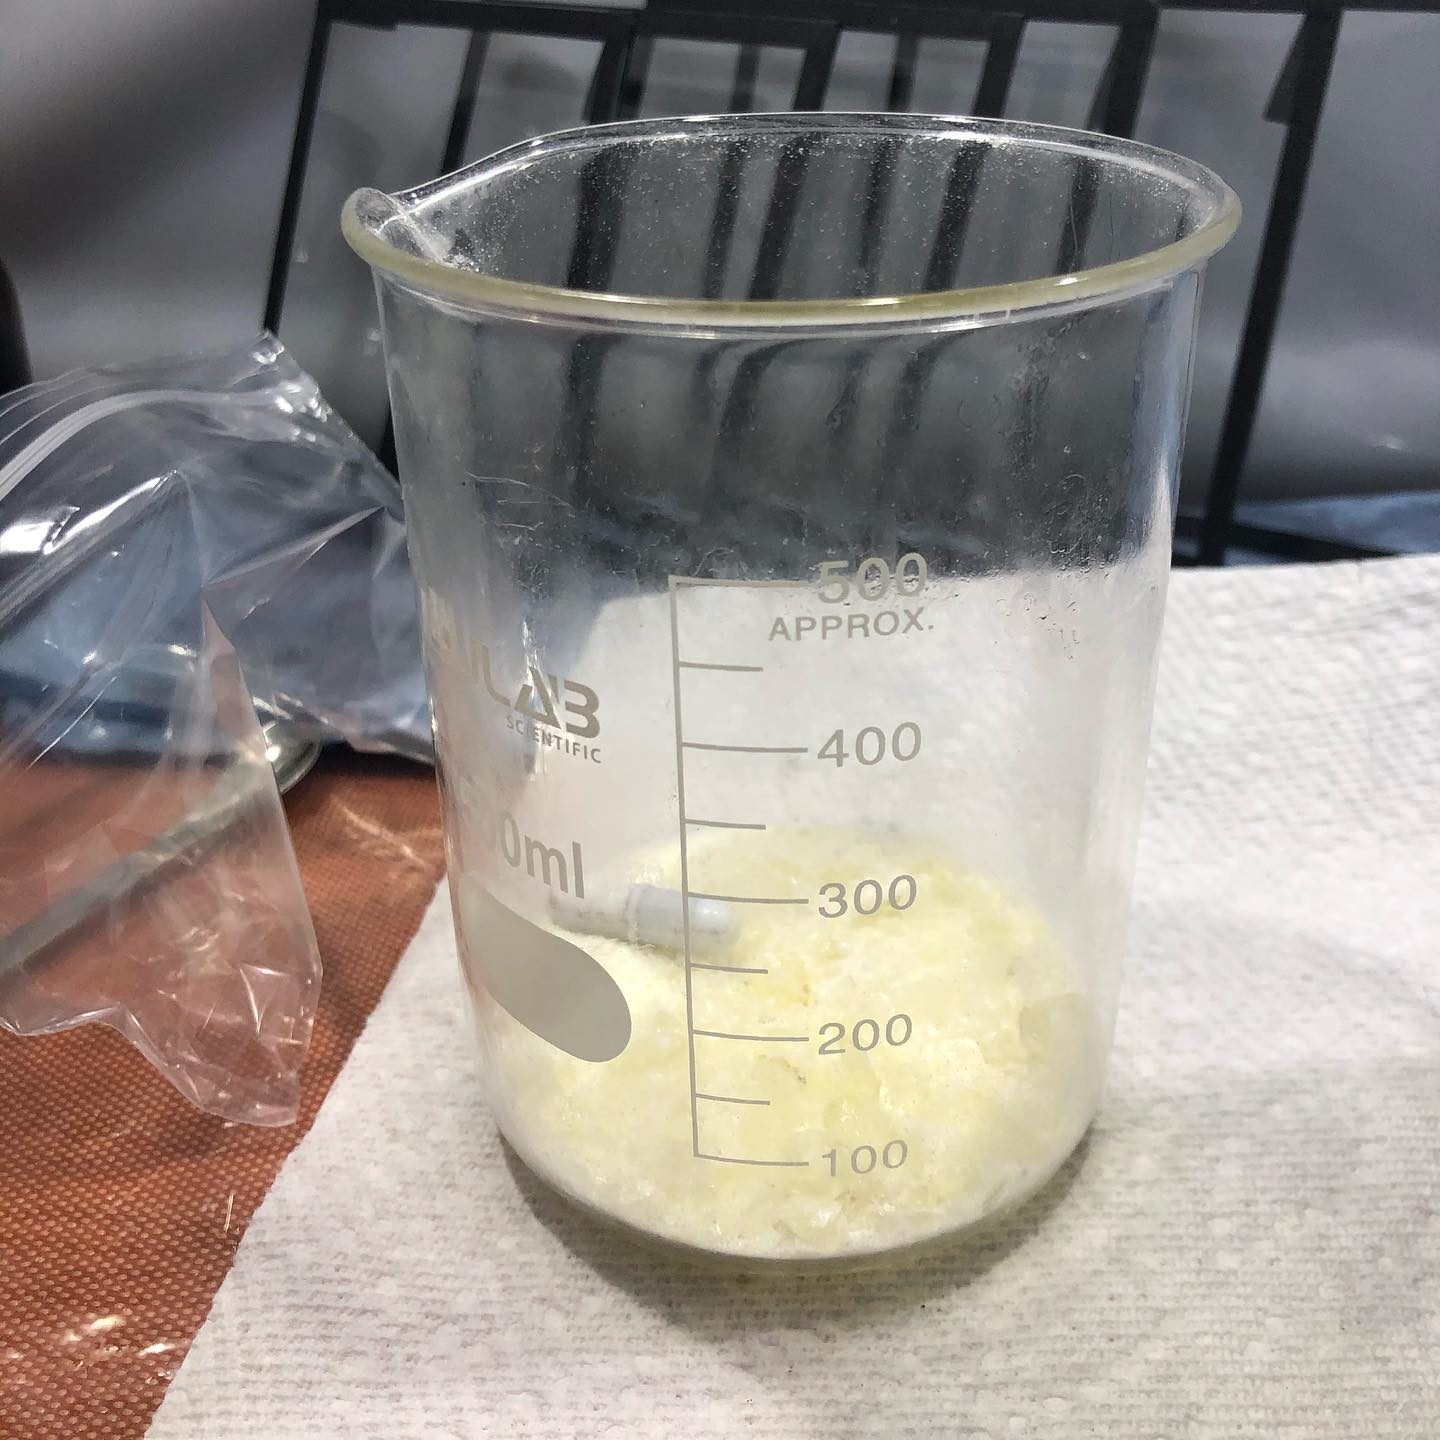
\includegraphics[width=4cm, height=4cm]{img/part1_36.jpg}
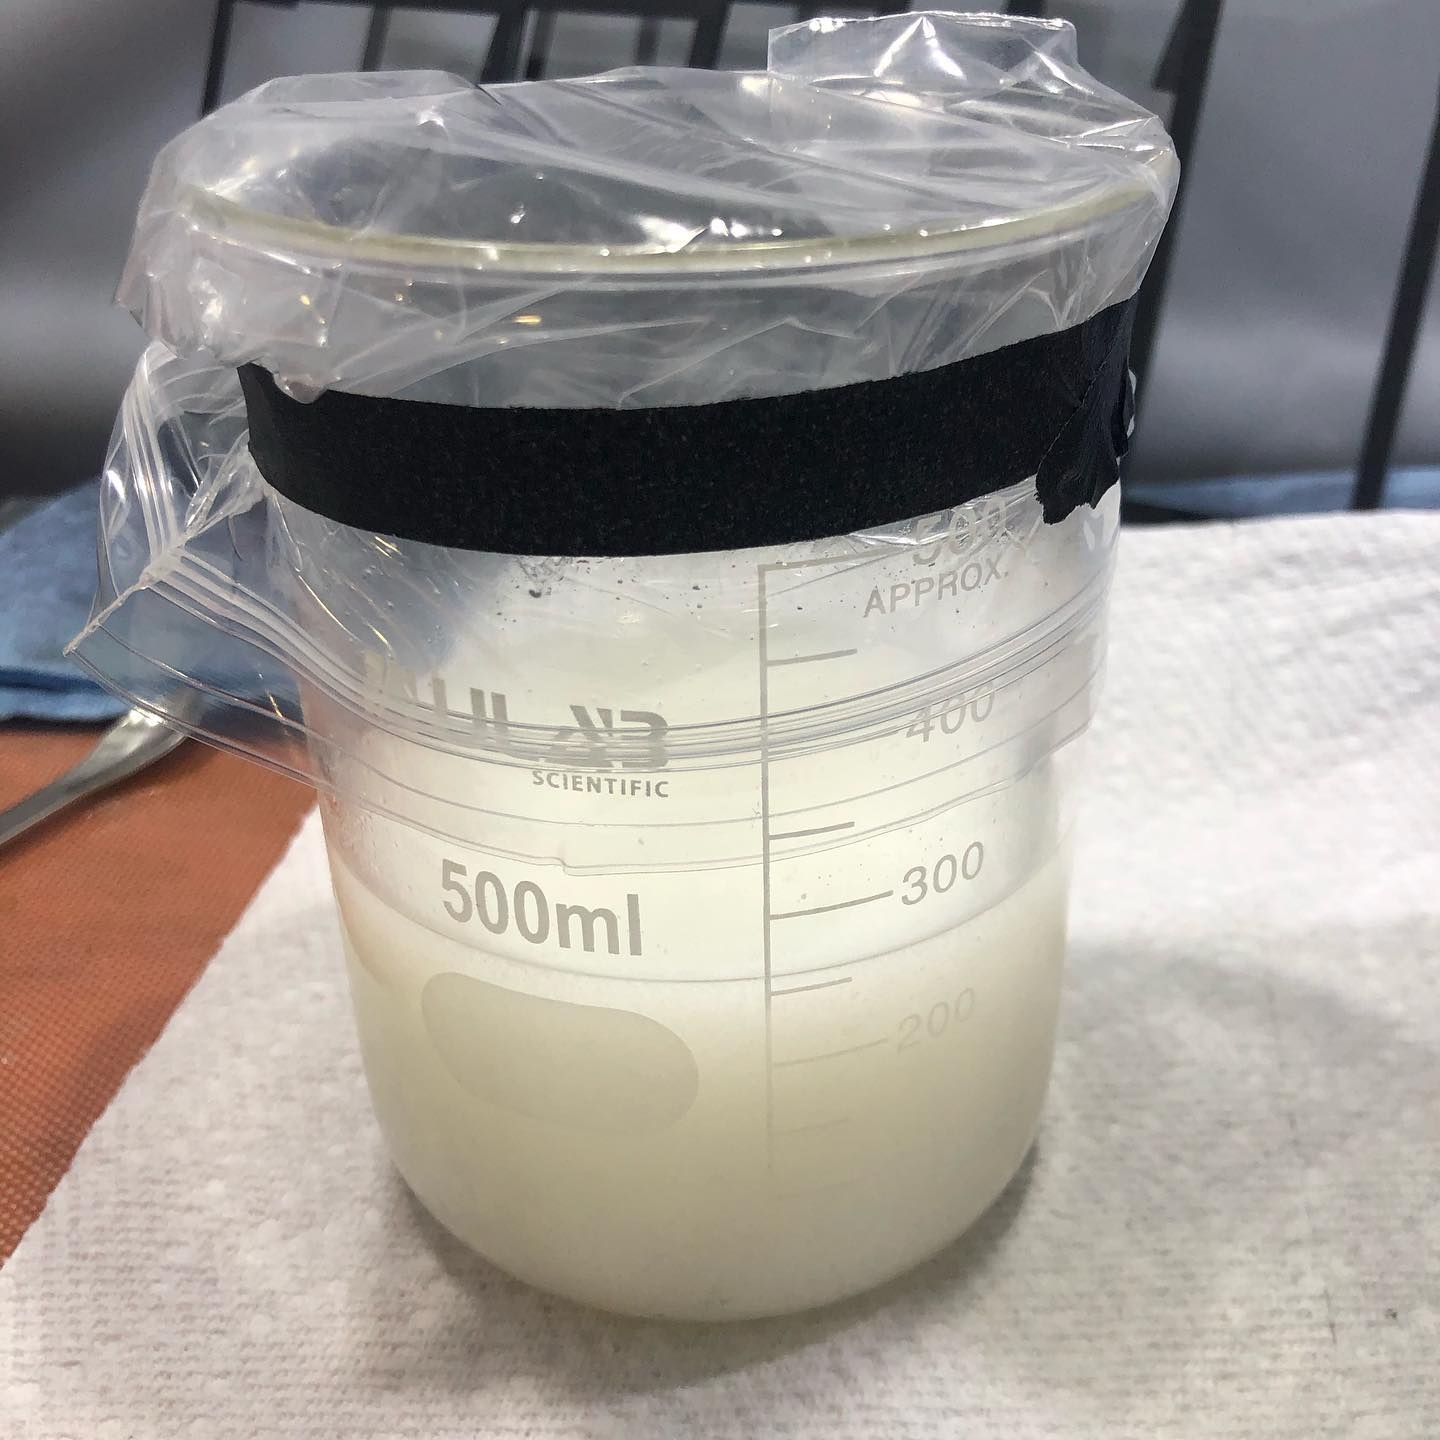
\includegraphics[width=4cm, height=4cm]{img/part1_37.jpg}
\end{center}

Now, we're going to filter out the beta-resene. Carefully filter the solution through two or three stacked coffee filters. After it has mostly filtered through, wash the filtrate with 50mL of ethyl acetate just to make sure. That takes care of 99\% of the beta-resene, but you'll likely notice that there are still tiny particles of the stuff that made it through. Carefully filter the solution again through 8-10 micron filter paper to remove the tiny bits.\newline
 
Time to add the nitrocellulose component. I buy pure lab-grade nitrocellulose from Ladd Research. For safety reasons, it has been wet with ethanol, to prevent it spontaneously combusting during shipping. If you plan on getting the same product I did, you're going to need to let a sample dry out first before measuring the weight.\newline

Add 7.2g of the nitrocellulose to the solution under magnetic stirring, and allow a couple of hours for it to dissolve.\newline

Finally, add 4.3mL of castor oil to the varnish, again with magnetic stirring. This should dissolve within a few seconds.  The castor oil acts as a plasticizer for the varnish.\newline

Now, with the remaining ethyl acetate, dilute the entire solution to about 500mL. Ideally, I like to shoot for a target of 0.40g dry varnish weight per 10mL of varnish. The exact final numbers will vary a bit, so you may need to adjust the final volume to get your numbers closer.\newline

\begin{center}
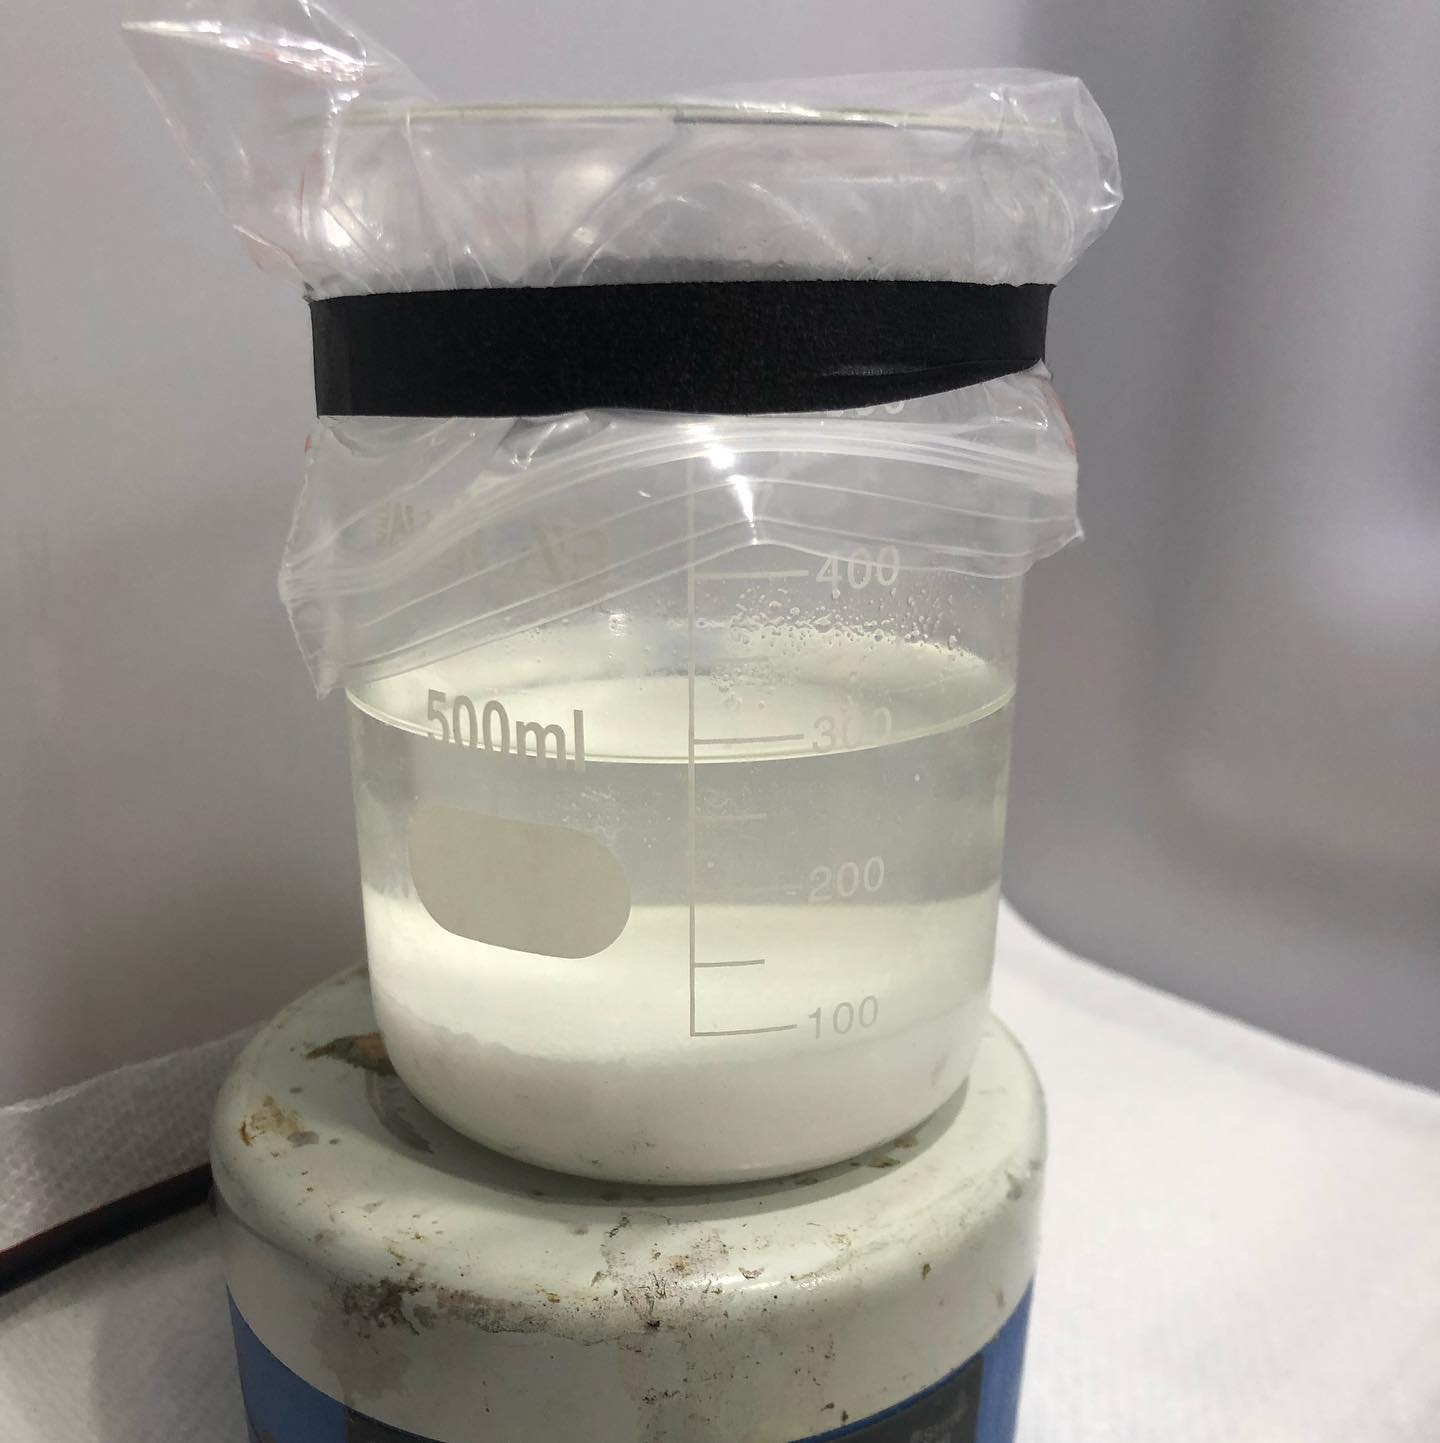
\includegraphics[width=5cm, height=5cm]{img/part1_38.jpg}
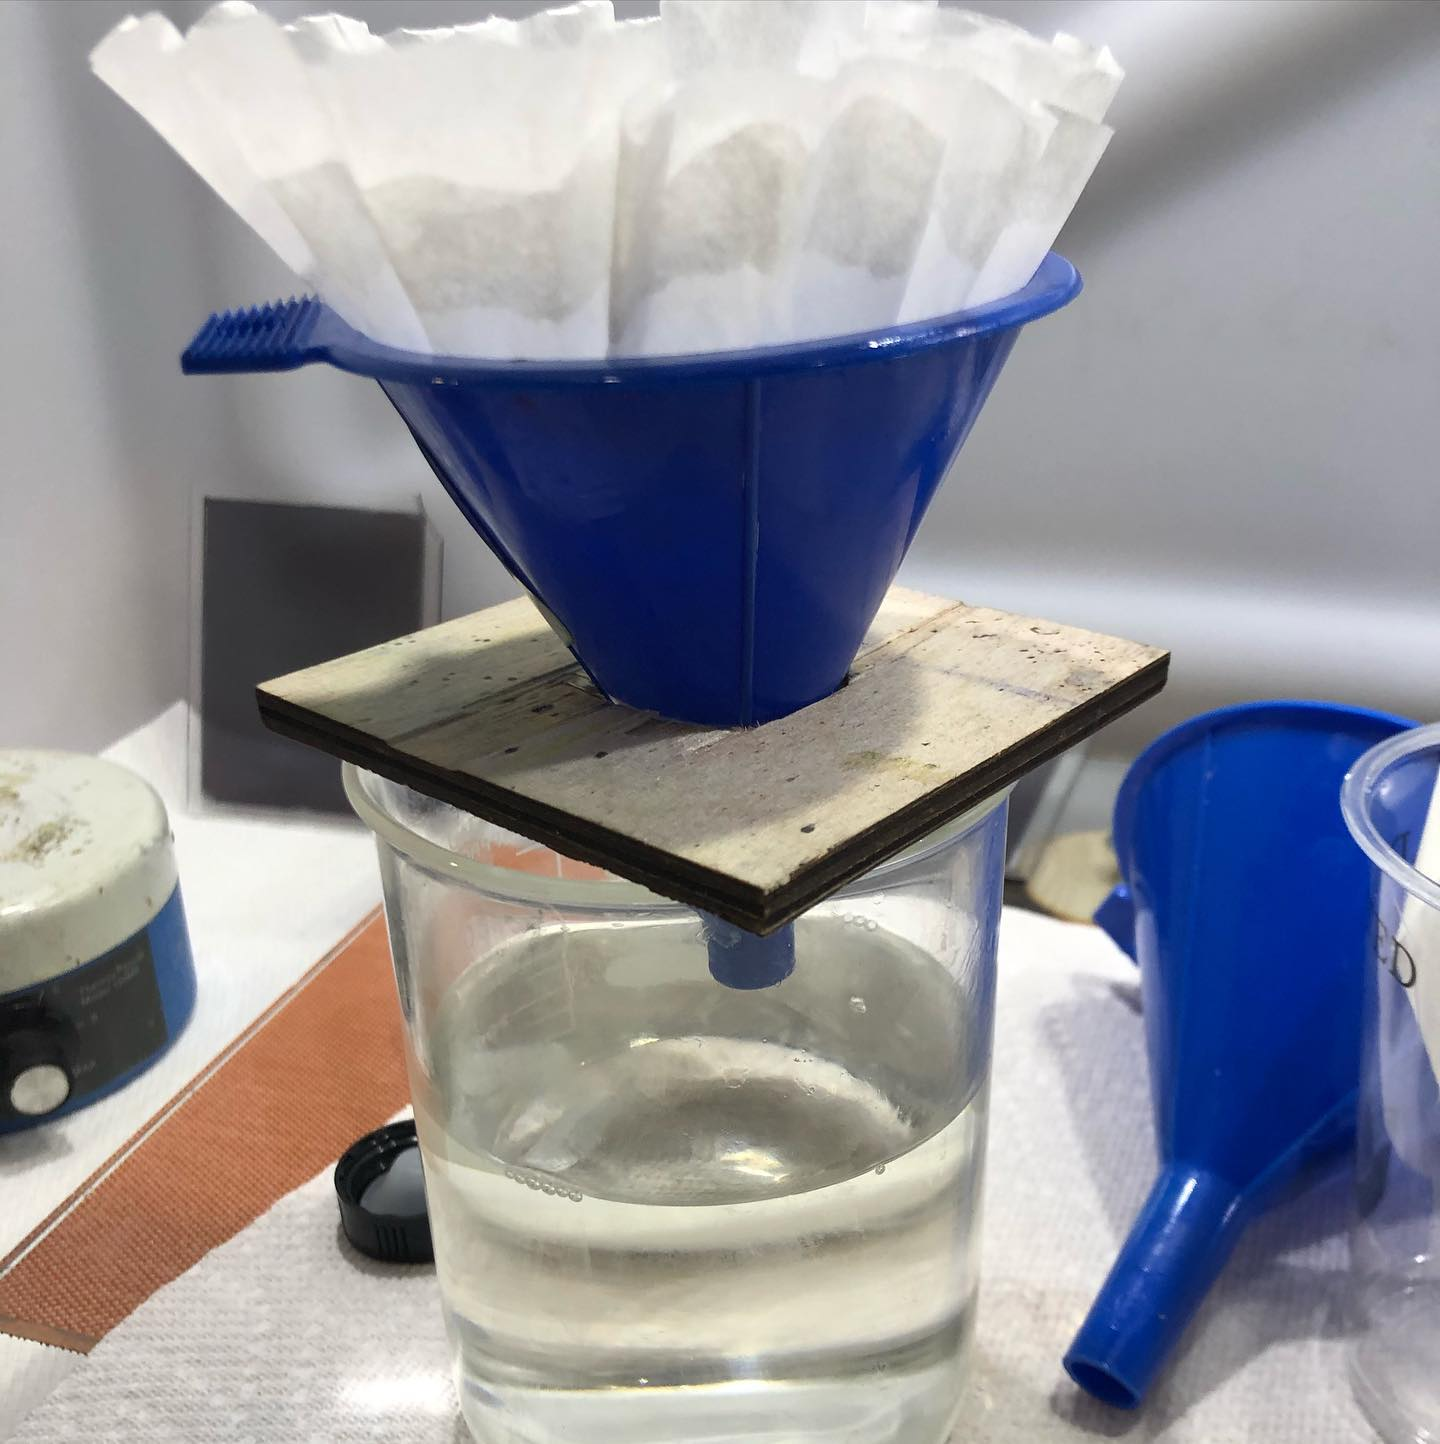
\includegraphics[width=5cm, height=5cm]{img/part1_39.jpg}
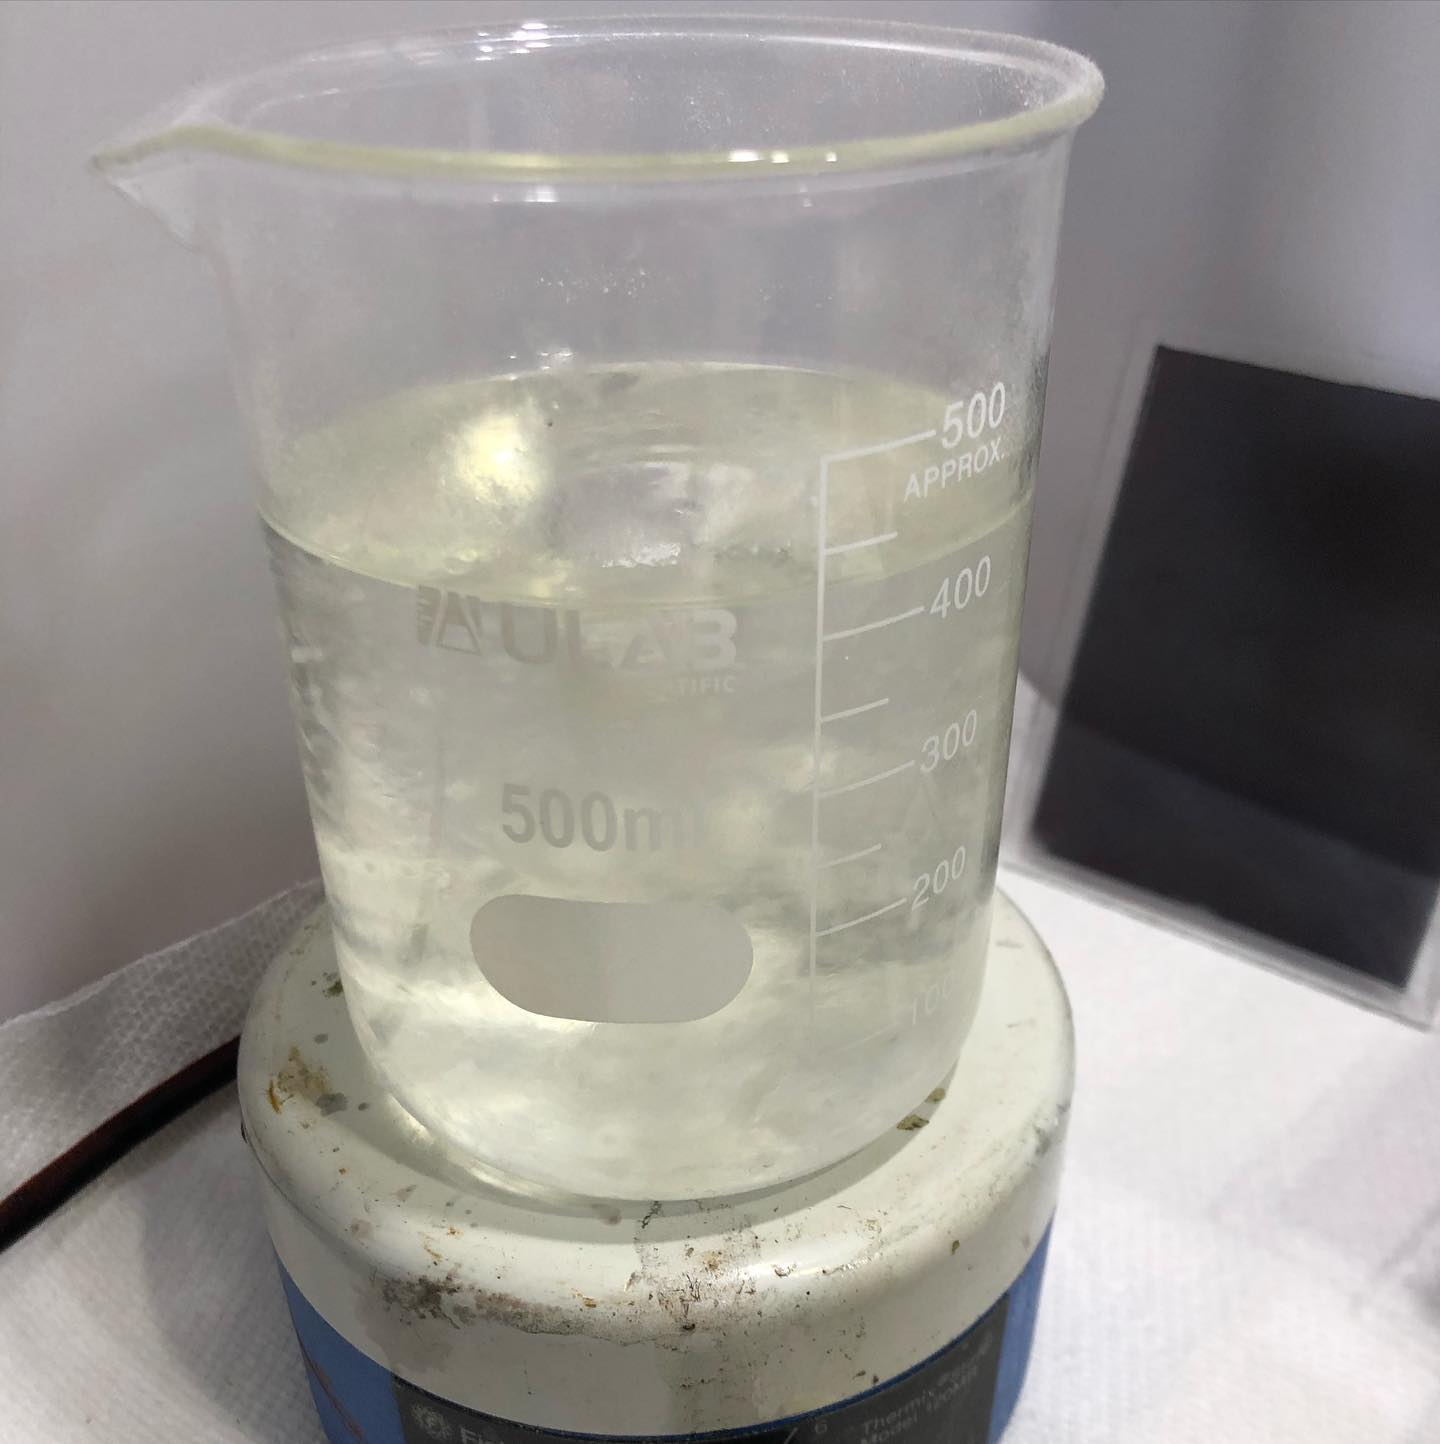
\includegraphics[width=5cm, height=5cm]{img/part1_40.jpg}
\end{center}

\subsection{Applying the Second Varnish}

I had a lot of trouble for a long time with this varnish. During tests, I would get opalescent clouding of the varnish as it dried, along with extensive formation of "wrinkles" which, along with being unsightly, tended to leak during tests. Ultimately, I was able to figure out that the extreme volatility of the ethyl acetate would cause the plate's temperature to drop sharply as it evaporated. Moisture from the air would condense into the varnish, pretty much screwing everything up. I played around with a dehumidifier, trying to make an intensely dry environment, though this did not seem to have much of an impact.\newline

Ultimately I was able to figure out that gentle heating, with the use of an adhesive silicone heating pad stuck beneath the leveling table, prevented these defects entirely. You don't want to use too high of a heat so as to cause the ethyl acetate to boil -- the goal is to keep the plate and varnish's temperature just above room temperature, to prevent moisture condensation. For my setup, I've found that setting the temperature controller to 35C seems to work best. I applied the heating pad to the bottom of some thick 1/4" glass.\newline

On a leveling table (leveled with a machinist's level, and ideally located in a fume hood or outside), set the screen down in cool portion of the glass, away from the heater. Dose 8mL of the Second Varnish to the center of the plate. With a small scoopula, help spread the meniscus of the varnish until full coverage is achieved. With care, gently slide the plate over the heated section with the scoopula, taking care to not disturb the meniscus and cause a spill. I prefer such a large meniscus, since it seems to produce a more even coating upon drying.\newline

Over the next 20 minutes or so, the varnish will rapidly dry, leaving behind a slightly tacky coating. Set aside to dry for about 8 hours or so (I usually leave it overnight), after which you should find it fairly hard.\newline

To test water-tightness of the coating, which is essential, you may want to place the plate in a dish for an hour and observe whether any leaks occurred. These should be fairly easy to spot, as the dyes will wash out quite easily.\newline

If you've made it this far, you've successfully made an autochrome screen plate! We're halfway there now, and you just need to make the light sensitive emulsion to rest on top.\newline

\begin{center}
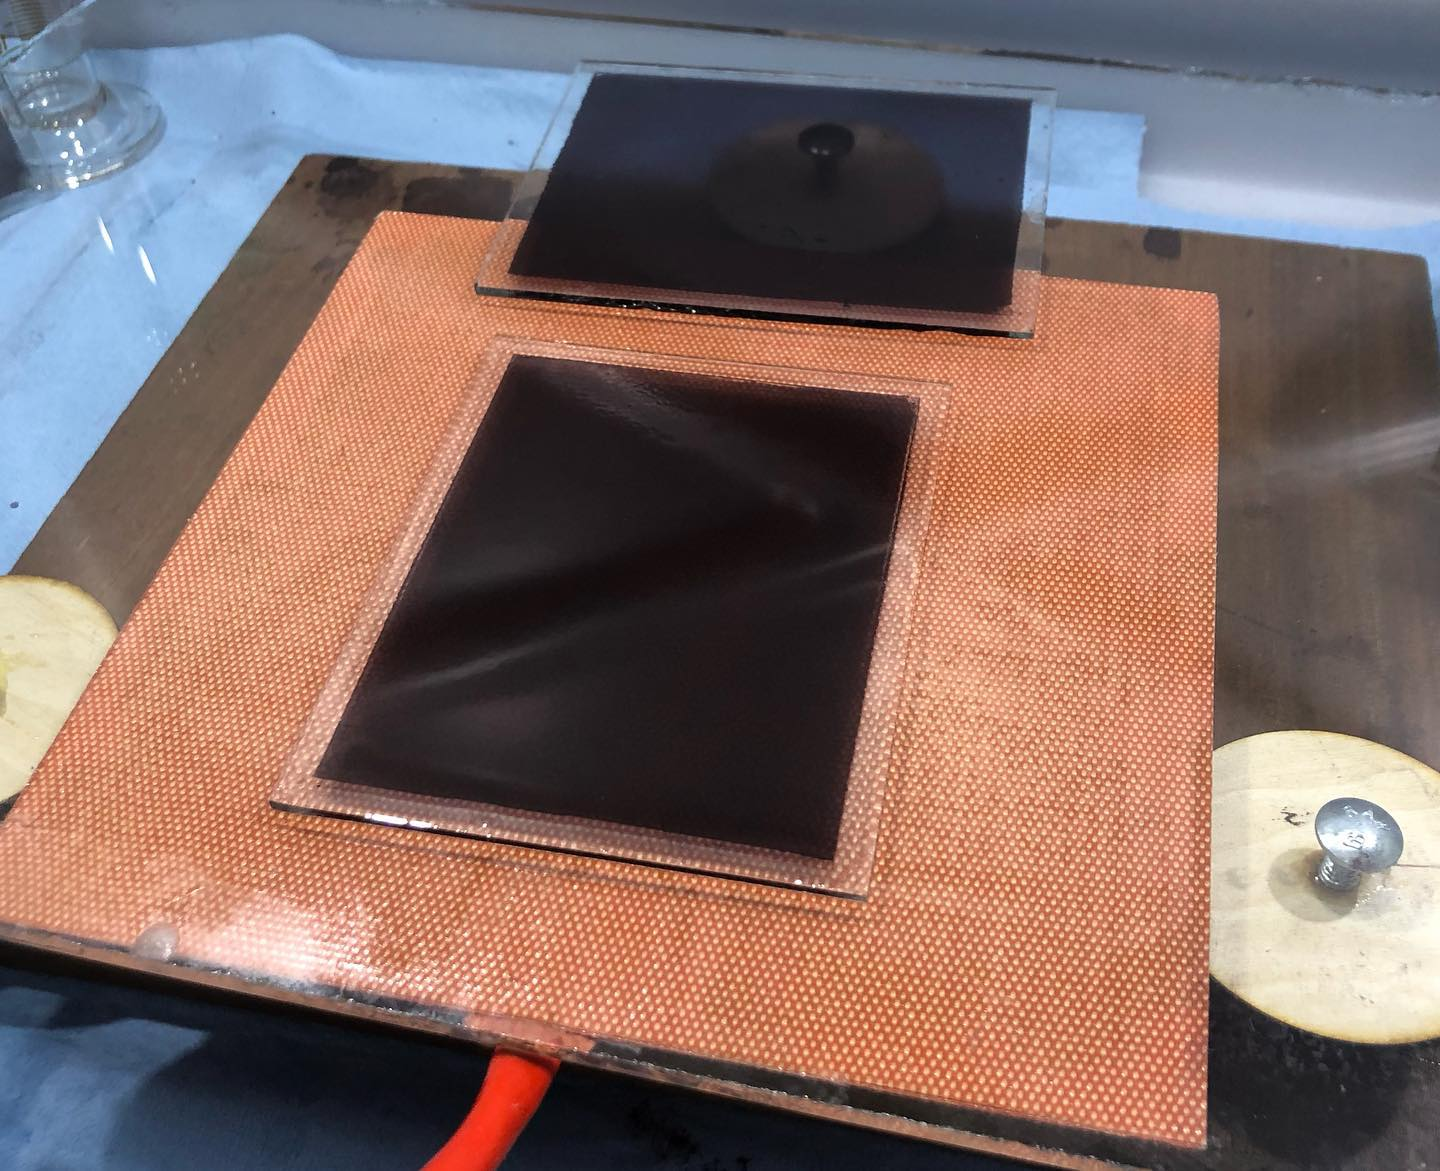
\includegraphics[width=4cm, height=4cm]{img/part1_41.jpg}
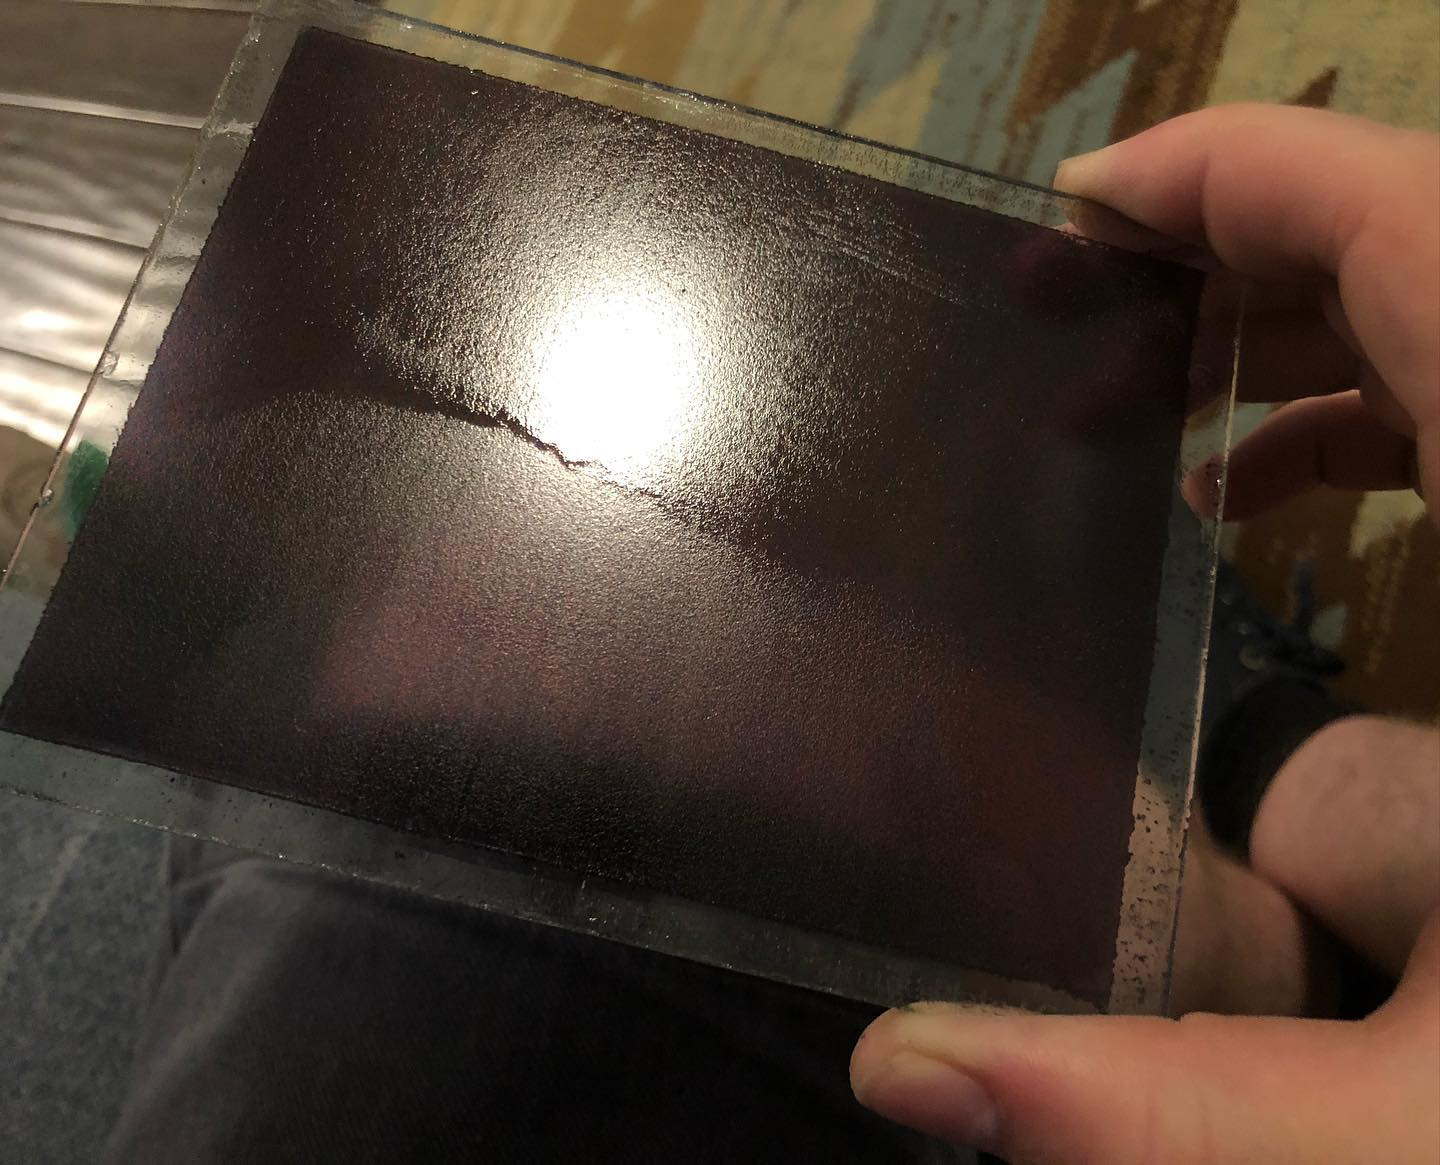
\includegraphics[width=4cm, height=4cm]{img/part1_42.jpg}
\includegraphics[width=4cm, height=4cm]{img/part1_43.jpg}
\includegraphics[width=4cm, height=4cm]{img/part1_44.jpg}
\end{center}

\pagebreak

\section{Making the Autochrome Emulsion}

If you've made it this far, congratulations! To make completed autochrome plate ready for exposure, we now have to make the light-sensitive layer, the "emulsion". I've been tweaking this recipe for a few years now, but it's by no means the definitive answer here. In fact, I wouldn't be surprised if a lot of different recipes would work here. The emulsion used here is a fairly straightforward black and white emulsion, with a couple of spectral sensitizers added in to make it panchromatic (sensitive to all wavelengths of the visible spectrum of light).\newline

In my experience, the most crucial characteristic is that the emulsion is thin, much thinner than what typical dry-plate practitioners might be used to. Thicker coatings will cause exposure times to climb, and tends to produce muddier colors. The emulsion coating must be extremely consistent from plate to plate as well, otherwise exposure times will vary wildly. Traditional hand coating techniques can't be used here very effectively, due to the extreme precision required for a successful coating.\newline

Due to the nature of an autochrome requiring a reversal processing, I also prefer to use a recipe with a fairly low contrast, since more typical recipes tend to result in fairly high contrast plates.\newline

As of the time I'm initially drafting this guide, this recipe is very slow compared to traditional autochromes. Exposure times in sunlight tend to vary anywhere between 10 seconds - 2 minutes, depending on the amount of color correction required. The speed of the emulsion can still be increased substantially, with the addition of gold+sulfur sensitization, and perhaps using an ammonia digest.\newline

The following chemicals will be required to make 400mL of this emulsion:
\begin{itemize}
	\item Silver Nitrate
	\item Ammonium Bromide
	\item Potassium Iodide
	\item 250 Bloom Photographic Gelatin
	\item Erythrosine Solution (1:1000, aqueous)
	\item Pinacyanol Solution (1:1000 in methanol)
	\item A few gallons of distilled water
\end{itemize}

In addition, I recommend having the following equipment on hand:
\begin{itemize}
	\item Hot Plate
	\item Magnetic Stirrer
	\item Spaghetti strainer
	\item Potato ricer
	\item Beakers (1000mL, 500mL, 2x 250mL)
	\item Syringe with interchangeable needle tip
\end{itemize}

\subsection{Precipitation}

Make the following solutions:\newline

\textbf{Solution A (500mL beaker)}

\begin{tabular}{ll}
	Ammonium Bromide & 7.42g \\
	Potassium Iodide 1\% Sln & 3mL \\
	Erythrosine* 1:1000. & 15mL \\
	Gelatin & 6.4g \\
	Distilled Water & 120mL \\
\end{tabular}\newline

\textbf{Solution B (250mL beaker)}

\begin{tabular}{ll}
	Silver Nitrate & 10.2g \\
	Distilled Water & 160mL \\
\end{tabular}\newline

1. Heat Solution B to 55C, with magnetic stirring (I use 300RPM), ensuring the gelatin has melted.

\textbf{From here on out, LIGHTS OUT}

2. Fill a syringe with a fine-needle tip with Solution B, and slowly add it to Solution A over the course of a few minutes. The solution should cloud up as the silver halides form.

3. Hold at 55C for 15 minutes.

4. Take off heat and place in a refrigerator to cool.

\subsection{Washing and Finals}

Under red safelights, remove the beaker of chilled emulsion after it has been cooling for several hours. Spoon out chunks, and shred them using a potato ricer. Shred the noodles into a large 1L beaker.\newline

Fill the beaker with distilled water, and mix with a spoon for a few seconds. Allow 10 minutes to soak, and then strain the noodles through a fine-meshed spaghetti strainer. After the noodles have been drained, scrape them back into the beaker and repeat the previous steps until you have completed four changes of water. Drain and add the noodles back to a 500mL beaker. You should have about 300mL of emulsion.\newline

From here, I split up the 300mL into 3 sets of 100mL batches. If you plan on using the whole batch, remember to adjust the following instructions accordingly.\newline

(Optional) Prepare a Steigmann's Solution, which consists of 25mL 1\% Ammonium Thiocyanate solution, and 3mL of a 1\% Gold Chloride solution. From this, take 10mL and add it to 200mL of distilled water. The Steigmann's solution will introduce gold and sulfur defects into the silver halide grains, hopefully increasing the speed of the emulsion.\newline 

In a 250mL beaker, heat the 100mL batch of emulsion to 55C. Add 6mL of the previously diluted Steigmann's solution to the emulsion, and hold for 60 minutes.\newline

Meanwhile, add 7.5g of gelatin to 300mL of distilled water to a 500mL beaker, and allow to swell. When the emulsion is done digesting, pour the emulsion into the gelatin solution, and heat back up to 45C to ensure all the gelatin has melted. When it reaches 45C, add 4mL* of 1:1000 pinacyanol and 2mL of 1\% chrome alum solution. Pinacyanol will render the emulsion sensitive to red, so be sure to use as little light as possible. Give it a few minutes of mixing, and then take it off heat for coating.\newline

\subsection{Coating the Screens}

Alright, this is going to be a little goofy. Due to the tight requirements for coating consistency required, normal coating technique can't really be used here very effectively. Plus, as you saw in the previous step, the emulsion is incredibly thin and runny, making it really hard to hold the plate and rock in your hand, as is traditionally done.\newline

First, a leveling table needs to be built. I slapped mine together with some parts from the hardware store -- all you need is to support a flat surface (I use glass 1/4" glass) by three screws. Using a machinist's level, level the glass as much as you can ahead of time.\newline

I also highly recommend using a 1-10mL variable pipette for dosing the emulsion, since it can be set ahead of time, and the built-in stops make it incredibly easy to use in the dark.\newline

Due to the red sensitivity of the emulsion, I recommend using as subdued of light as possible, while still being able to see what you're doing.\newline

For a 4x5 sized plate, dose 5mL of the emulsion to the center of the plate. Using your finger, spread the emulsion around until it has achieved full coverage, taking care not to spill any over the edge of the plate. With the far edge of the plate against the edge of the glass, rock the plate back and fourth for 5-10 seconds, before setting it level. It will depend on the ambient temperature, but allow the plates to set level for about 45 - 60 minutes to fully gel up, before placing them in a drying rack near some gentle air flow.\newline

\pagebreak

\section{Preparing to Expose the Autochrome Plate}

\textbf{The Ground Glass}\newline

Autochromes requires some slight modification to be shot on conventional large format hardware, due to the fact that the plates are exposed backwards. You will need to modify your ground glass to account for the shift in focal plane. I would recommend cutting some glass from the same stock that the autochrome plates are made from. Grinding the glass is surprisingly easy!  I use just a little bit of water and a spoonful of 600 grit silicon carbide tumbling powder.\newline

I recommend checking out this video \href{https://www.youtube.com/watch?v=hxC48_sd6BM}{here}, for further tips and instructions.\newline

\begin{center}
\includegraphics[width=5cm, height=5cm]{img/part3_1.jpg}
\includegraphics[width=5cm, height=5cm]{img/part3_2.jpg}
\end{center}

\textbf{The Plate Holder}\newline

Right now, since I personally use 3/32" (single-strength) glass, the plates don't always work 100\% with older plate holders. Out of the last 3 holders I purchased, two slots were offset slightly, resulting in out-of-focus exposures. Your mileage may vary.\newline

Personally, I prefer to use "Premo" packfilm holders, with a 3d printed insert I designed originally for Lippmann plates. The insert holds the plate nice and snug against the holder, resulting in crystal clear shots every time.\newline

I have made my design publicly available for modification or download \href{https://www.tinkercad.com/things/66n26SZCvrX}{here}.\newline

Remember: AUTOCHROME PLATES ARE LOADED GLASS-SIDE TOWARDS THE LENS!\newline

\begin{center}
\includegraphics[width=5cm, height=5cm]{img/part3_3.jpg}
\includegraphics[width=5cm, height=5cm]{img/part3_4.jpg}
\end{center}

\textbf{Color Corrective Filters}\newline

If you absolutely nail the color response from the emulsion, there's no actual need for filters during exposure. However, I've found that this is exceedingly difficult to do, and that the plates tend to have a bias towards a color. In addition to color shifts, oversensitivity to a particular color results in washed colors with low saturation.\newline

I use a Cibachrome CMY filter kit with 9x9 sized filters to dial in the color balance for each batch of emulsion. The 3d printed filter holder I designed is also available for modification or download \href{https://www.tinkercad.com/things/iRrxHK9En0b}{here}.\newline

\begin{center}
\includegraphics[width=5cm, height=5cm]{img/part3_5.jpg}
\includegraphics[width=5cm, height=5cm]{img/part3_6.jpg}
\includegraphics[width=5cm, height=5cm]{img/part3_7.jpg}
\end{center}

\subsection{Exposing the Autochrome Plate}

There are an unbelievable amount of variables when it comes to making the emulsion, so I can't exactly tell you what your exposure time will be with any amount of accuracy. I can, however, give a few benchmarks that I use when I'm dialing in exposure parameters for a new batch of emulsion. I highly recommend the use of a spot meter here, as well as some good note taking skills.\newline

Without any extra filtration, exposures on an EV14 (a colorful object in sunny conditions) tend to be around 10-20 seconds. Plates requiring heavy color correction (my current batch, as of writing, are heavily biased towards green and blue and require 50Y+40M filters) exposures tend to be around 1m45s.\newline

Correct exposure here is more important than, say, a typical negative process, since the autochrome doesn't have the same amount of exposure latitude. Small to medium errors in brightness can be corrected for later with intensification or reduction, but the best results will be obtained with the correct exposure time.\newline

\subsection{Processing the Autochrome Plate}

The following baths are required for developing the autochrome plate.\newline

\textbf{D-19 (Stock, dissolve compounds in the order listed)}\newline

\begin{tabular}{ll}
	Distilled Water & 1000mL \\
	Metol & 2g \\
	Sodium Sulfite & 90g \\
	Hydroquinone & 8g \\
	Sodium Carbonaten & 52.5g (monohydrate) or 43.5g (anhydrous)\\
	Potassium Bromide & 5g
\end{tabular}\newline

\href{http://stores.photoformulary.com/formulary-substitute-d-19/}{Photographer's Formulary Kit}\newline

\textbf{Potassium Thiocyanate (KSCN) 5\% Solution}\newline

\begin{tabular}{ll}
	Distilled Water & 500mL \\
	Potassium Thiocyanate & 9.5g \\
\end{tabular}\newline

\textbf{Reversal Bleach}\newline

\begin{tabular}{ll}
	Distilled Water & 1000mL \\
	Potassium Dichromate & 9.5g \\
	Sulfuric Acid (48\%) & 25mL \\
\end{tabular}\newline

\textbf{Clearing Bath}\newline

\begin{tabular}{ll}
	Distilled Water & 1000mL \\
	Sodium Sulfite & 50g \\
\end{tabular}\newline

The following baths are optional for processing, but are heavily recommended to have on hand at the time of development.\newline

\textbf{Superproportional Reducer}\newline

\begin{tabular}{ll}
	Distilled Water & 500mL \\
	Ammonium Persulfate & 25g \\
	Sulfuric Acid (48\%) & 6mL \\
\end{tabular}\newline

\href{http://stores.photoformulary.com/reducer-ii-for-negatives-ground-ups-only/}{Photographer's Formulary Kit}\newline

\textbf{Chromium Intensifier}\newline

\begin{tabular}{ll}
	Distilled Water & 250mL \\
	Potassium Dichromate & 50g \\
	Hydrochloric Acid (38\%) & 6mL \\
\end{tabular}\newline

1. \textbf{First Development.} The first developer can be made with 25mL D-19 Stock + 75mL distilled water + 5mL 5\% KSCN solution. This usually is enough to cover one 4x5 sized plate in a 5x7 sized tray. With the lights completely off, gently develop the plate for 2m30s. The developer may be used for multiple plates, but should be disposed of when you're done for the day, or it begins to visibly turn yellow.\newline

2.Rinse with tap water for 30s - 2 minutes. After the plate has been thoroughly rinsed, it's okay to turn on the white lights.\newline

3. \textbf{Reversal Bleach.} Place the plate in a tray of the reversal bleach. If made fresh, the action of the bleach can be extremely rapid, and may only take a few seconds. An older bath may take upwards of two minutes. The solution is incredibly shelf stable, and a small bath of it can be used on dozens of plates. I prefer to keep a small amount in a glass tray with a lid, to reduce the amount I have to pour it, since potassium dichromate is somewhat hazardous. You can't overdo this step, only underdo it.\newline

4.Rise thoroughly with tap water\newline

5. \textbf{Clearing Bath.} Place the plate in a tray of fresh sodium sulfite. This will neutralize the orange chromium VI, turning it to a safer green chromium III. The bath may be used for several plates, but should be disposed of after you're done for the day. You can't overdo this step, only underdo it.\newline

6.Rinse thoroughly with tap water. At this point, the colors can be viewed if you so choose. They should be fairly weak, but visible.\newline

7. \textbf{Second Development.} Place the plate in a bath of stock D-19. The plate should darken over the course of a few minutes. You can't overdo this step, only underdo it.\newline

8.Final rinse.\newline

\begin{center}
\includegraphics[width=4cm, height=4cm]{img/part3_8.jpg}
\includegraphics[width=4cm, height=4cm]{img/part3_9.jpg}
\includegraphics[width=4cm, height=4cm]{img/part3_10.jpg}
\includegraphics[width=4cm, height=4cm]{img/part3_11.jpg}
\end{center}

\textbf{Reduction (optional).} Inspect the plate via transmission with a light bulb. Is the plate too dark, with somewhat muddy colors? You might improve things with the superproportional developer I described earlier. To make the working solution, ad 30mL of the reducer stock to 70mL of water. You can eyeball this, the measurements aren't super critical. I would recommend against the use of Farmer's Reducer here, as it tends to completely nuke the highlights.\newline

Submerse the plate in the bath with gentle agitation. After 1 minute, pull the plate and observe the image. If more reduction is required, continue to agitate, observing the plate at 30 second intervals. The reducer starts out slow, but will start to work exponentially faster the longer you reduce for, so watch out! The emulsion will start to turn from black to dark brown as you reduce. Reduce until it juuuust looks right, and then wash with tap water to remove the reducer. Let the plate sit in the clearing bath for 2 or so minutes, and then rinse again and set it to dry.\newline

%Link to video1

\textbf{Intensification (optional).} You may find that after second development, your plate looks overexposed, with blown out colors. You may want to try intensifying the plate. I don't have as much experience intensifying plates, but I've found the best results were obtained with a chromium intensifier. A few plates that were hopelessly overexposed were rescued after several back and fourths between intensifying and redevelopment in D-19. I won't be writing the full procedure through here, as this is still fairly experimental. I have found that many plates I have intensified tended to leak at the edges, and I think the bath may be causing the second varnish to lift from the glass somewhat. Your mileage may vary.\newline

\textbf{Top Coat and Mounting.} The autochromes usually seem to be stable after drying, but I still recommend applying a topcoat to the plate, or risk peeling/cracking over the next few weeks. I prefer to use "Eagle" brand acrylic gloss varnish, which is a UV-resistant solvent based acrylic driveway sealer. Apply 5-6mL in the center of your completed plate, and rock the plate around until full coverage is achieved. Set level to dry overnight. It will be tacky for a day or so, and I prefer to let the coating gas out for at least a week before mounting the plate against another piece of glass. It will depend on the thickness, but when it comes time to mount the plate against another piece of glass, I just use normal black 3/4" masking tape, running along the edges.\newline

\end{document}
